% Plot Catalog - 20 Comprehensive Supplementary Plots
\documentclass[11pt]{article}

\usepackage[utf8]{inputenc}
\usepackage[T1]{fontenc}
\usepackage{graphicx}
\usepackage[margin=0.5in]{geometry}
\usepackage{hyperref}
\usepackage{xcolor}

\hypersetup{
    colorlinks=true,
    linkcolor=blue,
    citecolor=blue,
    urlcolor=blue,
}

\graphicspath{{paper_figures/supplementary_v2/}}

\title{Plot Catalog: 20 Supplementary Visualization Options}
\author{Browse and Select Your Favorites}
\date{\today}

\begin{document}

\maketitle

\section*{Overview}

This catalog presents 20 different visualization approaches for the derivative estimation benchmark data. Each plot addresses specific aspects of the data and uses different techniques to handle the extreme nRMSE range (10$^{-9}$ to 10$^{22}$).

\textbf{Key improvements over initial plots:}
\begin{itemize}
    \item Shows more methods (not just top 5)
    \item Uses log scales to avoid ``smushing'' (better dynamic range)
    \item Multiple complementary perspectives
    \item Various stratifications (by order, noise, category, etc.)
\end{itemize}

\textbf{Browse and choose:} Select the plots that best support your paper's narrative and colleague presentations.

\clearpage

%==============================================================================
% PLOT 1
%==============================================================================

\section*{Plot 1: Box Plots - All Methods}

\textbf{What it shows:} Distribution of log10(nRMSE) for all 27 methods across all conditions

\textbf{Strengths:}
\begin{itemize}
    \item Shows complete picture (all methods)
    \item Reveals outliers and spread
    \item Horizontal layout easier to read than vertical
    \item Clear ranking by median performance
\end{itemize}

\textbf{Best for:} Overall method comparison, identifying consistent vs variable methods

\begin{figure}[h]
\centering
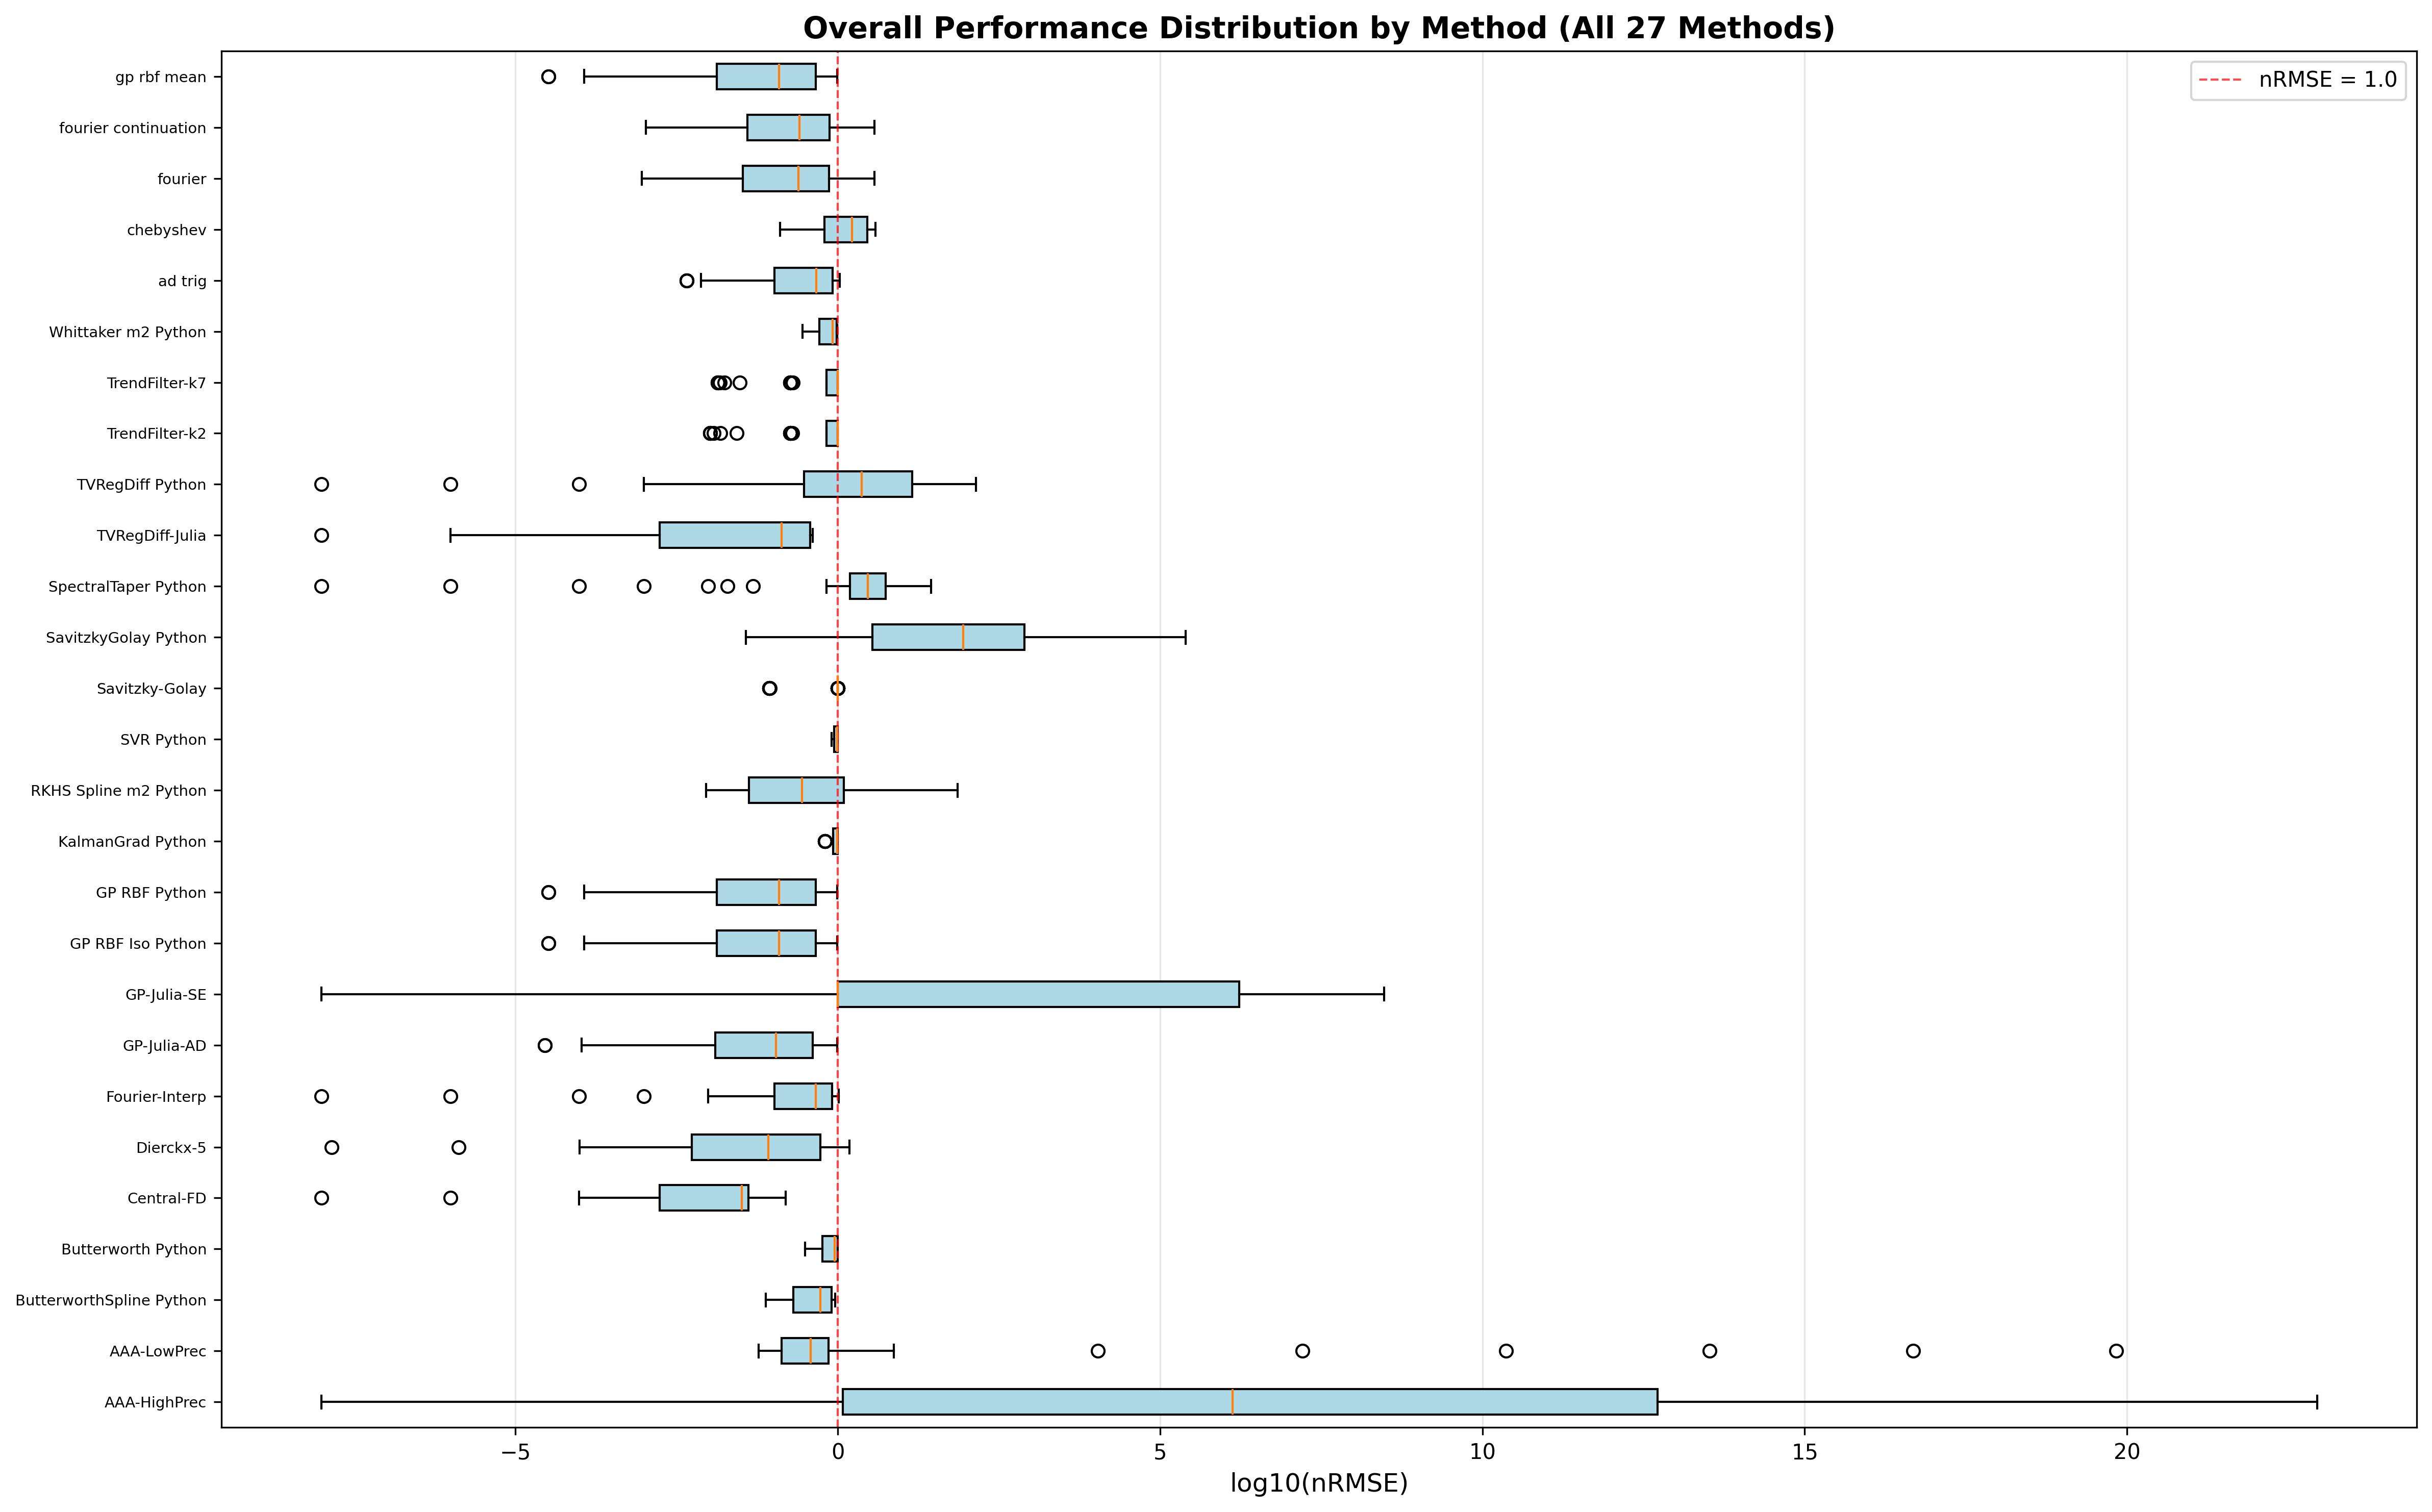
\includegraphics[width=\textwidth]{plot01_boxplot_all_methods.png}
\end{figure}

\clearpage

%==============================================================================
% PLOT 2
%==============================================================================

\section*{Plot 2: Line Plot - Performance Degradation with Order}

\textbf{What it shows:} How log10(nRMSE) increases with derivative order (all 16 full-coverage methods)

\textbf{Strengths:}
\begin{itemize}
    \item Clearly shows ``order is primary difficulty driver''
    \item All full-coverage methods visible
    \item Can identify catastrophic failures (steep jumps)
    \item Legend allows method identification
\end{itemize}

\textbf{Best for:} Demonstrating order effect, AAA catastrophic failure at order 3+

\begin{figure}[h]
\centering
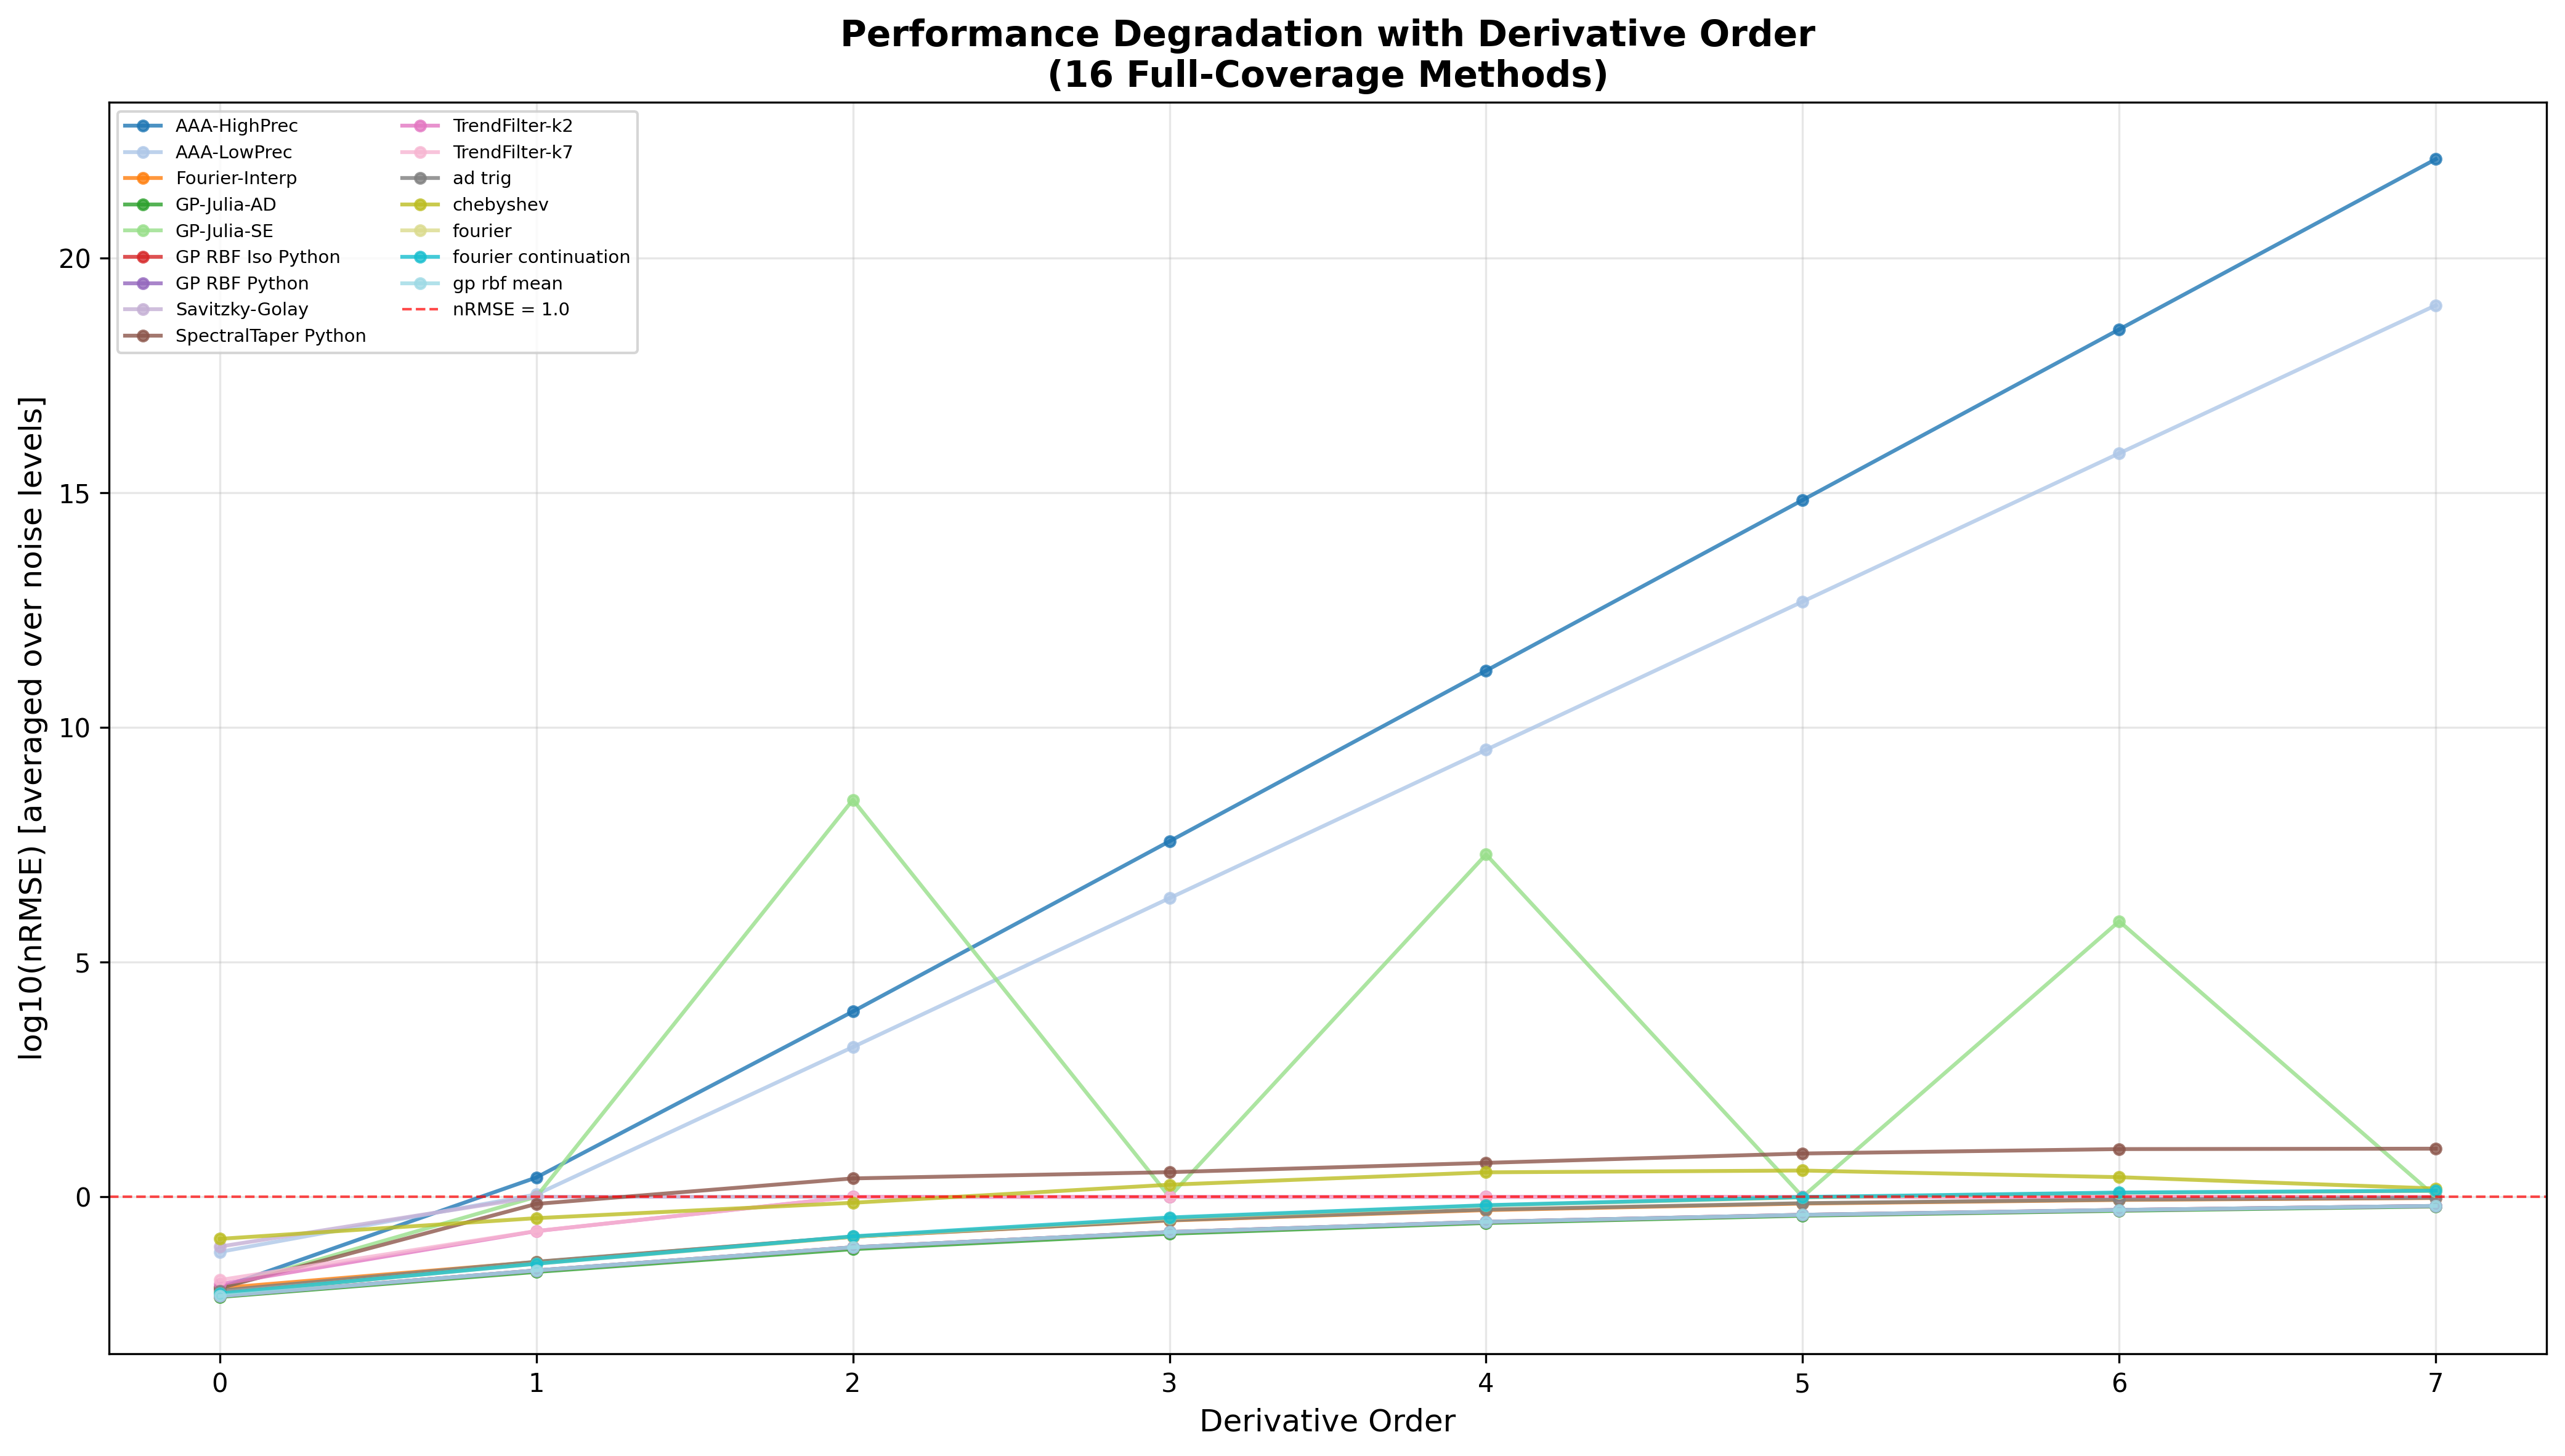
\includegraphics[width=\textwidth]{plot02_line_order_all_methods.png}
\end{figure}

\clearpage

%==============================================================================
% PLOT 3
%==============================================================================

\section*{Plot 3: Heatmap - Method vs Order}

\textbf{What it shows:} log10(nRMSE) for all methods across derivative orders (averaged over noise)

\textbf{Strengths:}
\begin{itemize}
    \item Compact visualization of method × order performance
    \item Color gradient reveals patterns quickly
    \item All 27 methods visible
    \item Easy to spot method clusters (good/bad at high orders)
\end{itemize}

\textbf{Best for:} High-level overview, pattern recognition

\begin{figure}[h]
\centering
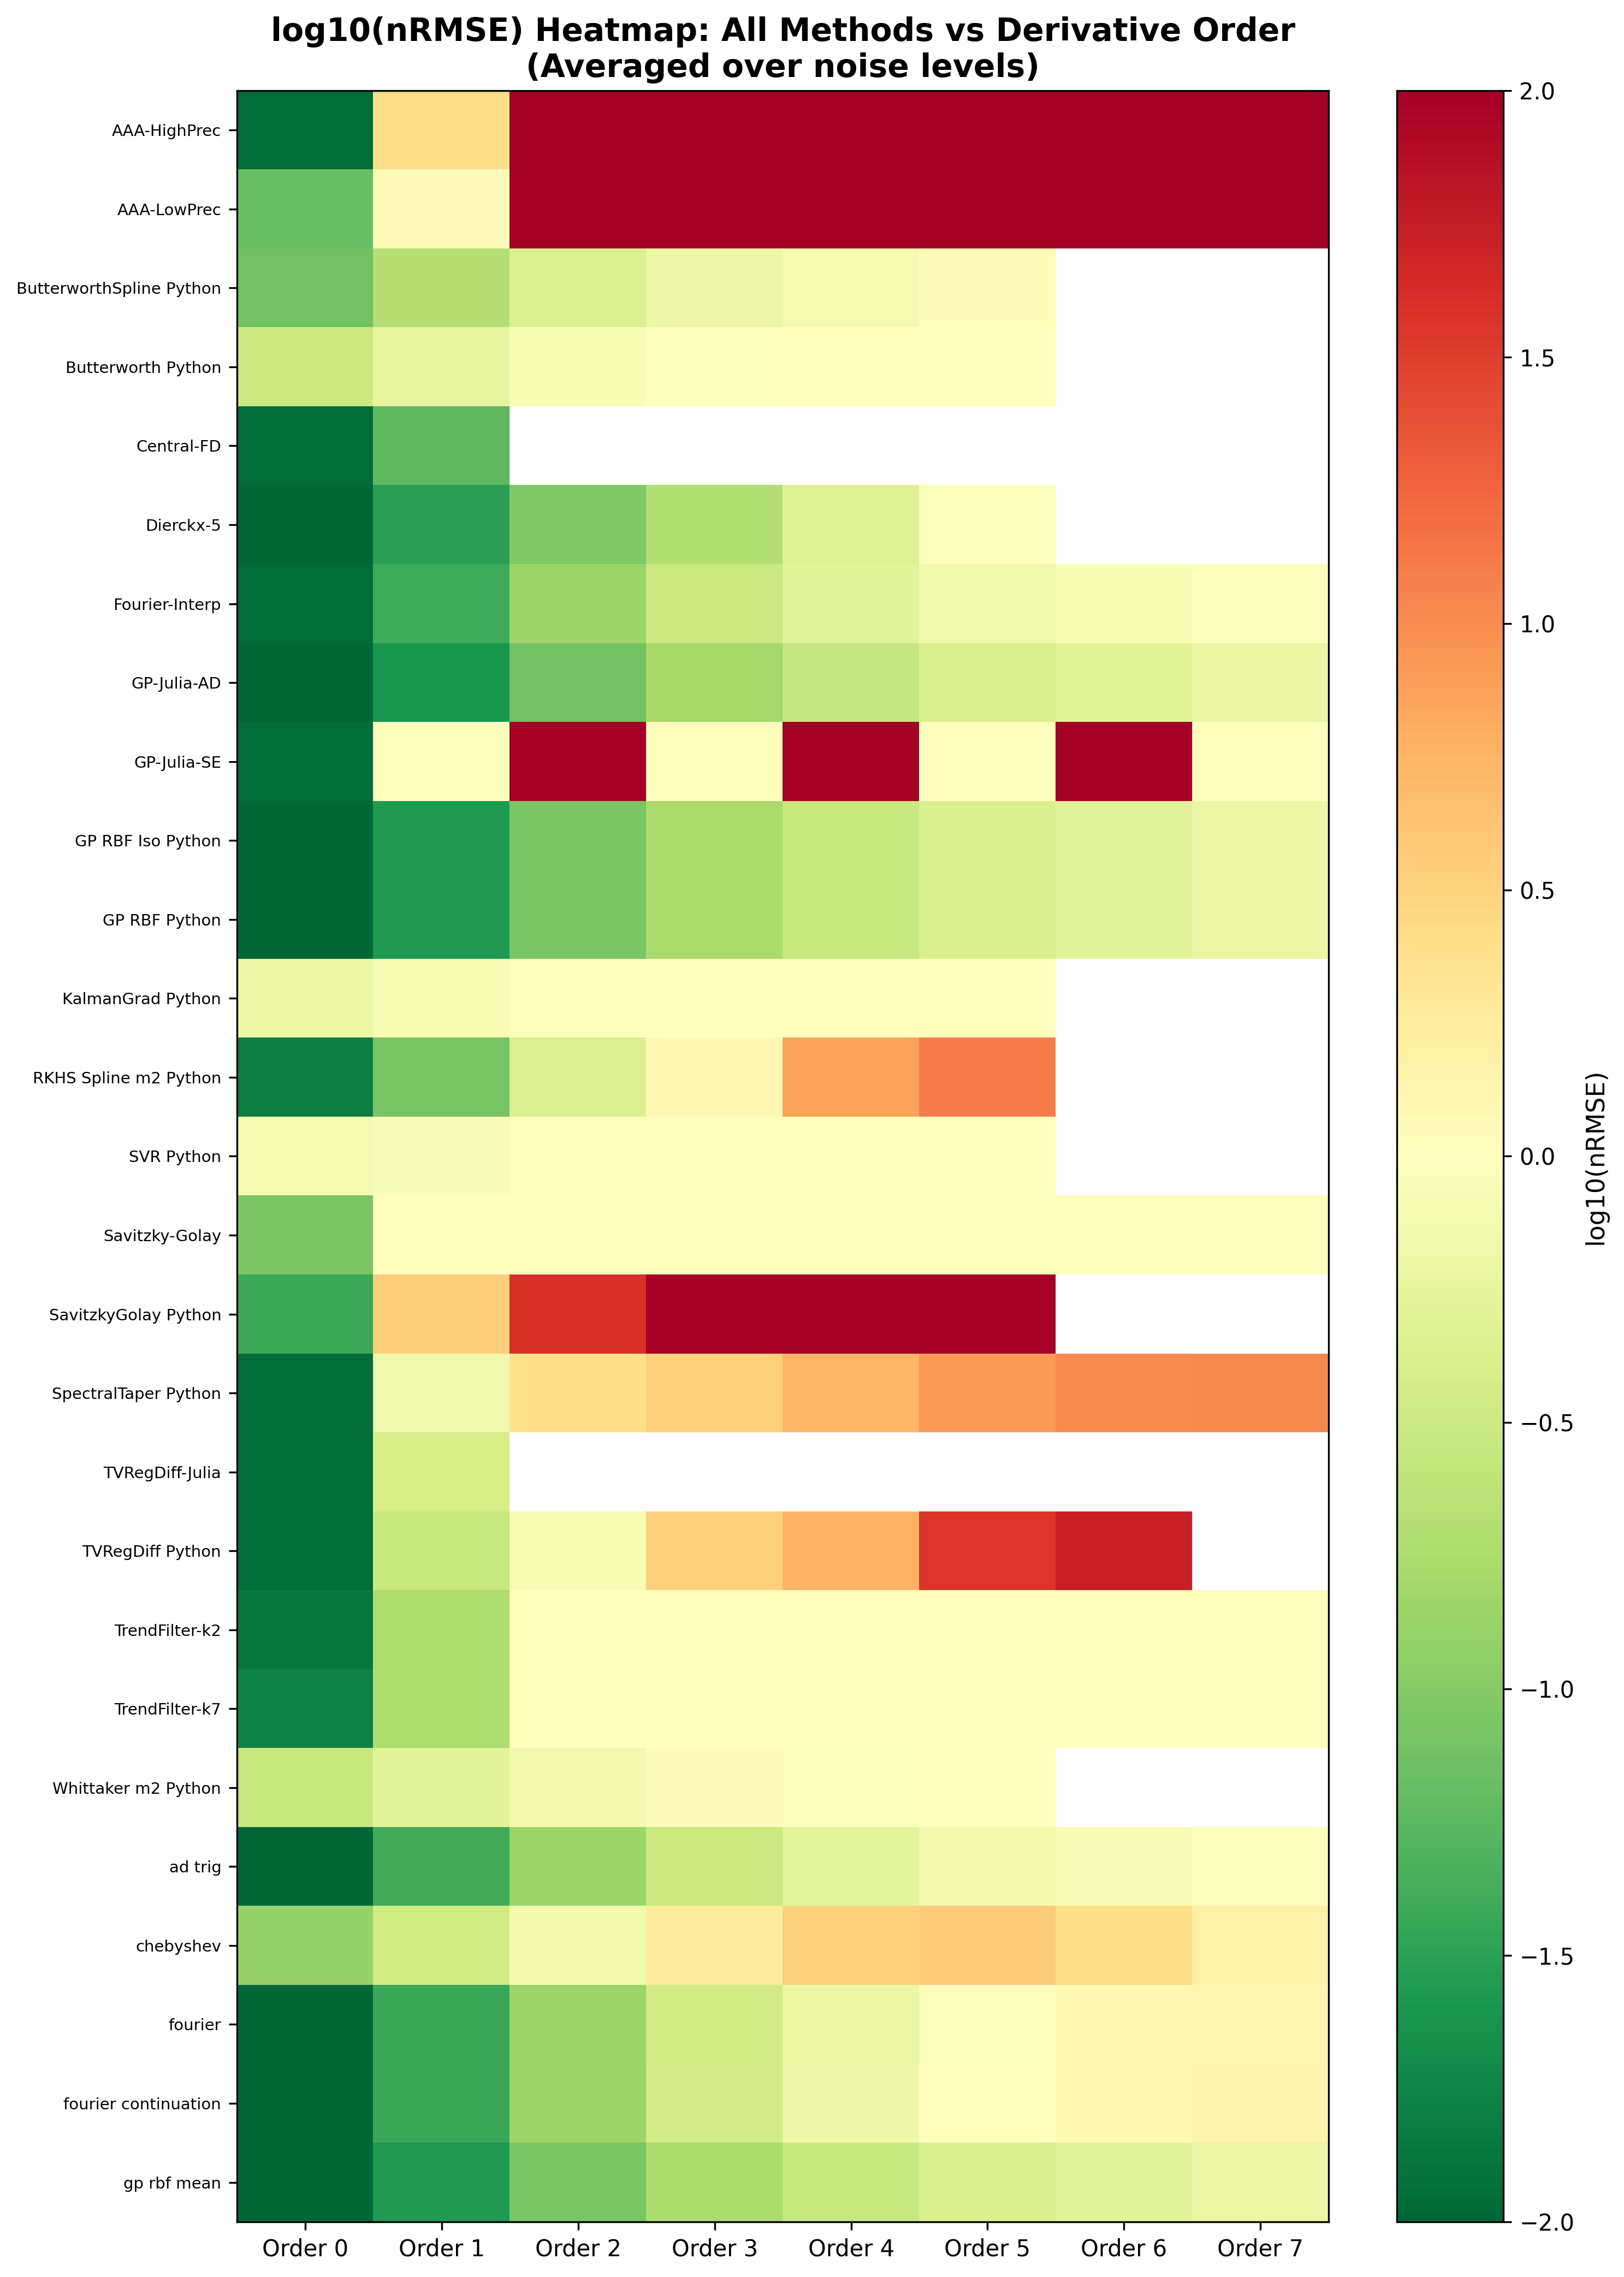
\includegraphics[width=0.85\textwidth]{plot03_heatmap_method_order.png}
\end{figure}

\clearpage

%==============================================================================
% PLOT 4
%==============================================================================

\section*{Plot 4: Small Multiples - Noise Sensitivity by Order}

\textbf{What it shows:} log10(nRMSE) vs noise level, one panel per derivative order

\textbf{Strengths:}
\begin{itemize}
    \item Shows all full-coverage methods (16 lines)
    \item Reveals noise sensitivity patterns at each order
    \item Can identify methods with flat vs steep noise curves
    \item Comprehensive view of method behavior
\end{itemize}

\textbf{Best for:} Detailed noise sensitivity analysis, method selection for specific noise levels

\begin{figure}[h]
\centering
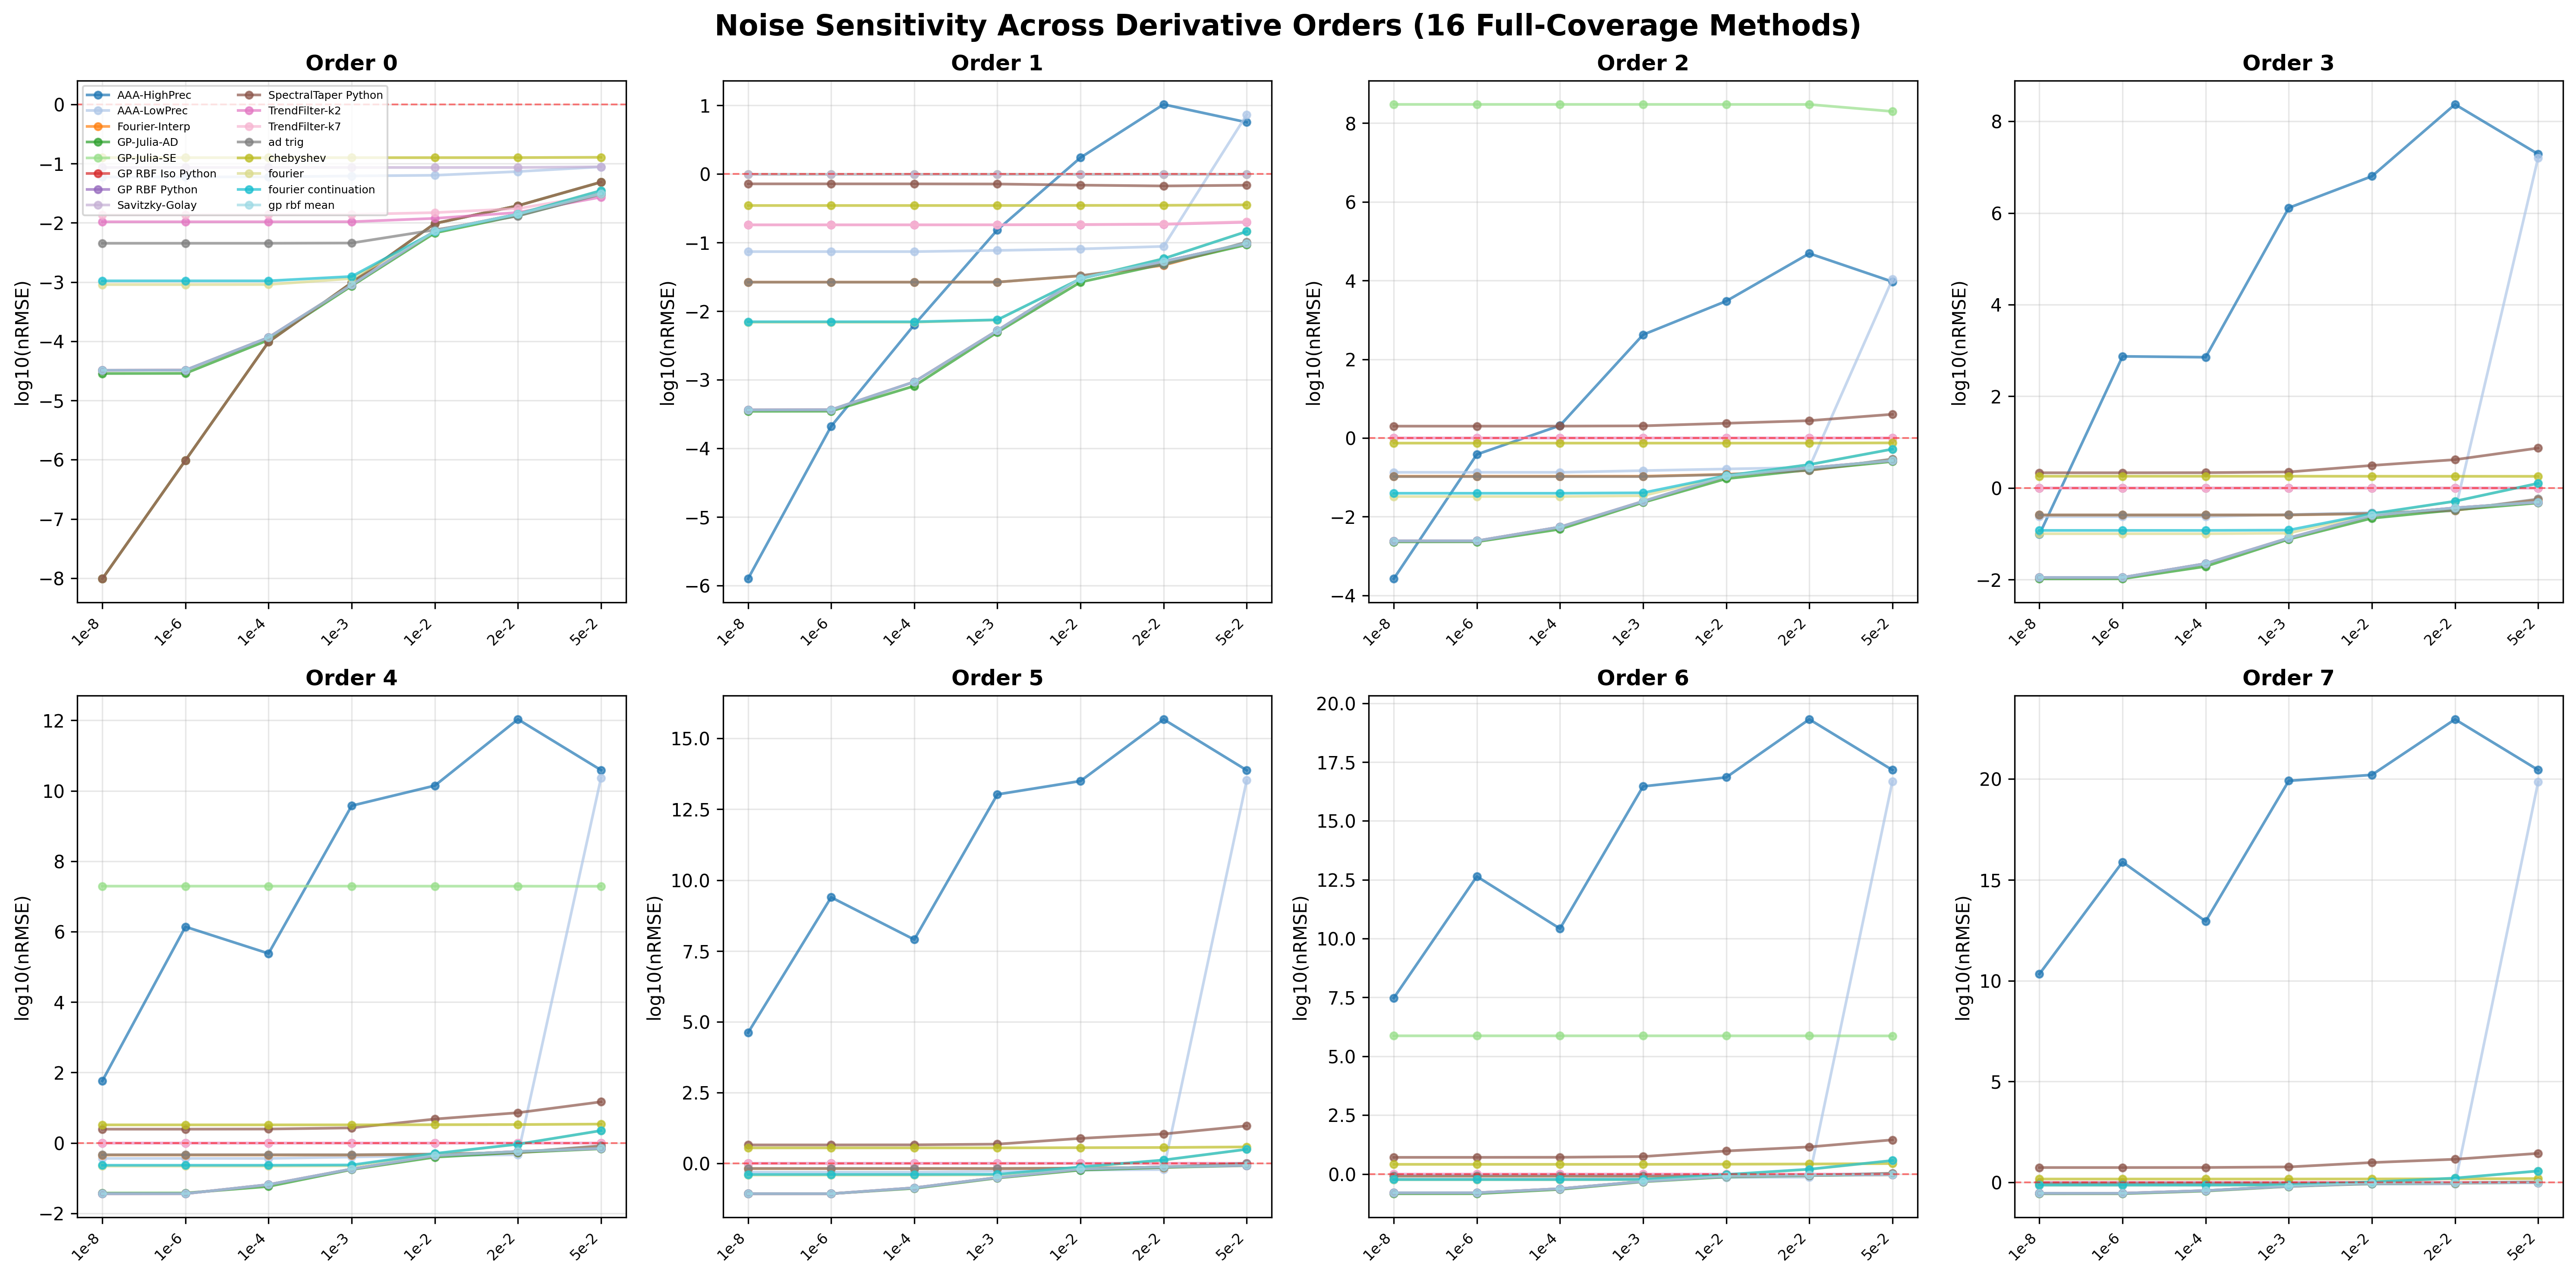
\includegraphics[width=\textwidth]{plot04_small_multiples_noise.png}
\end{figure}

\clearpage

%==============================================================================
% PLOT 5
%==============================================================================

\section*{Plot 5: Rank Bar Chart}

\textbf{What it shows:} Mean log10(nRMSE) for all methods, sorted from best to worst

\textbf{Strengths:}
\begin{itemize}
    \item Simple, clear ranking
    \item Color-coded (green/orange/red) for quick assessment
    \item Shows GP-Julia-AD as top performer
    \item Easy to see performance tiers
\end{itemize}

\textbf{Best for:} Quick reference, supporting ``best method'' claims

\begin{figure}[h]
\centering
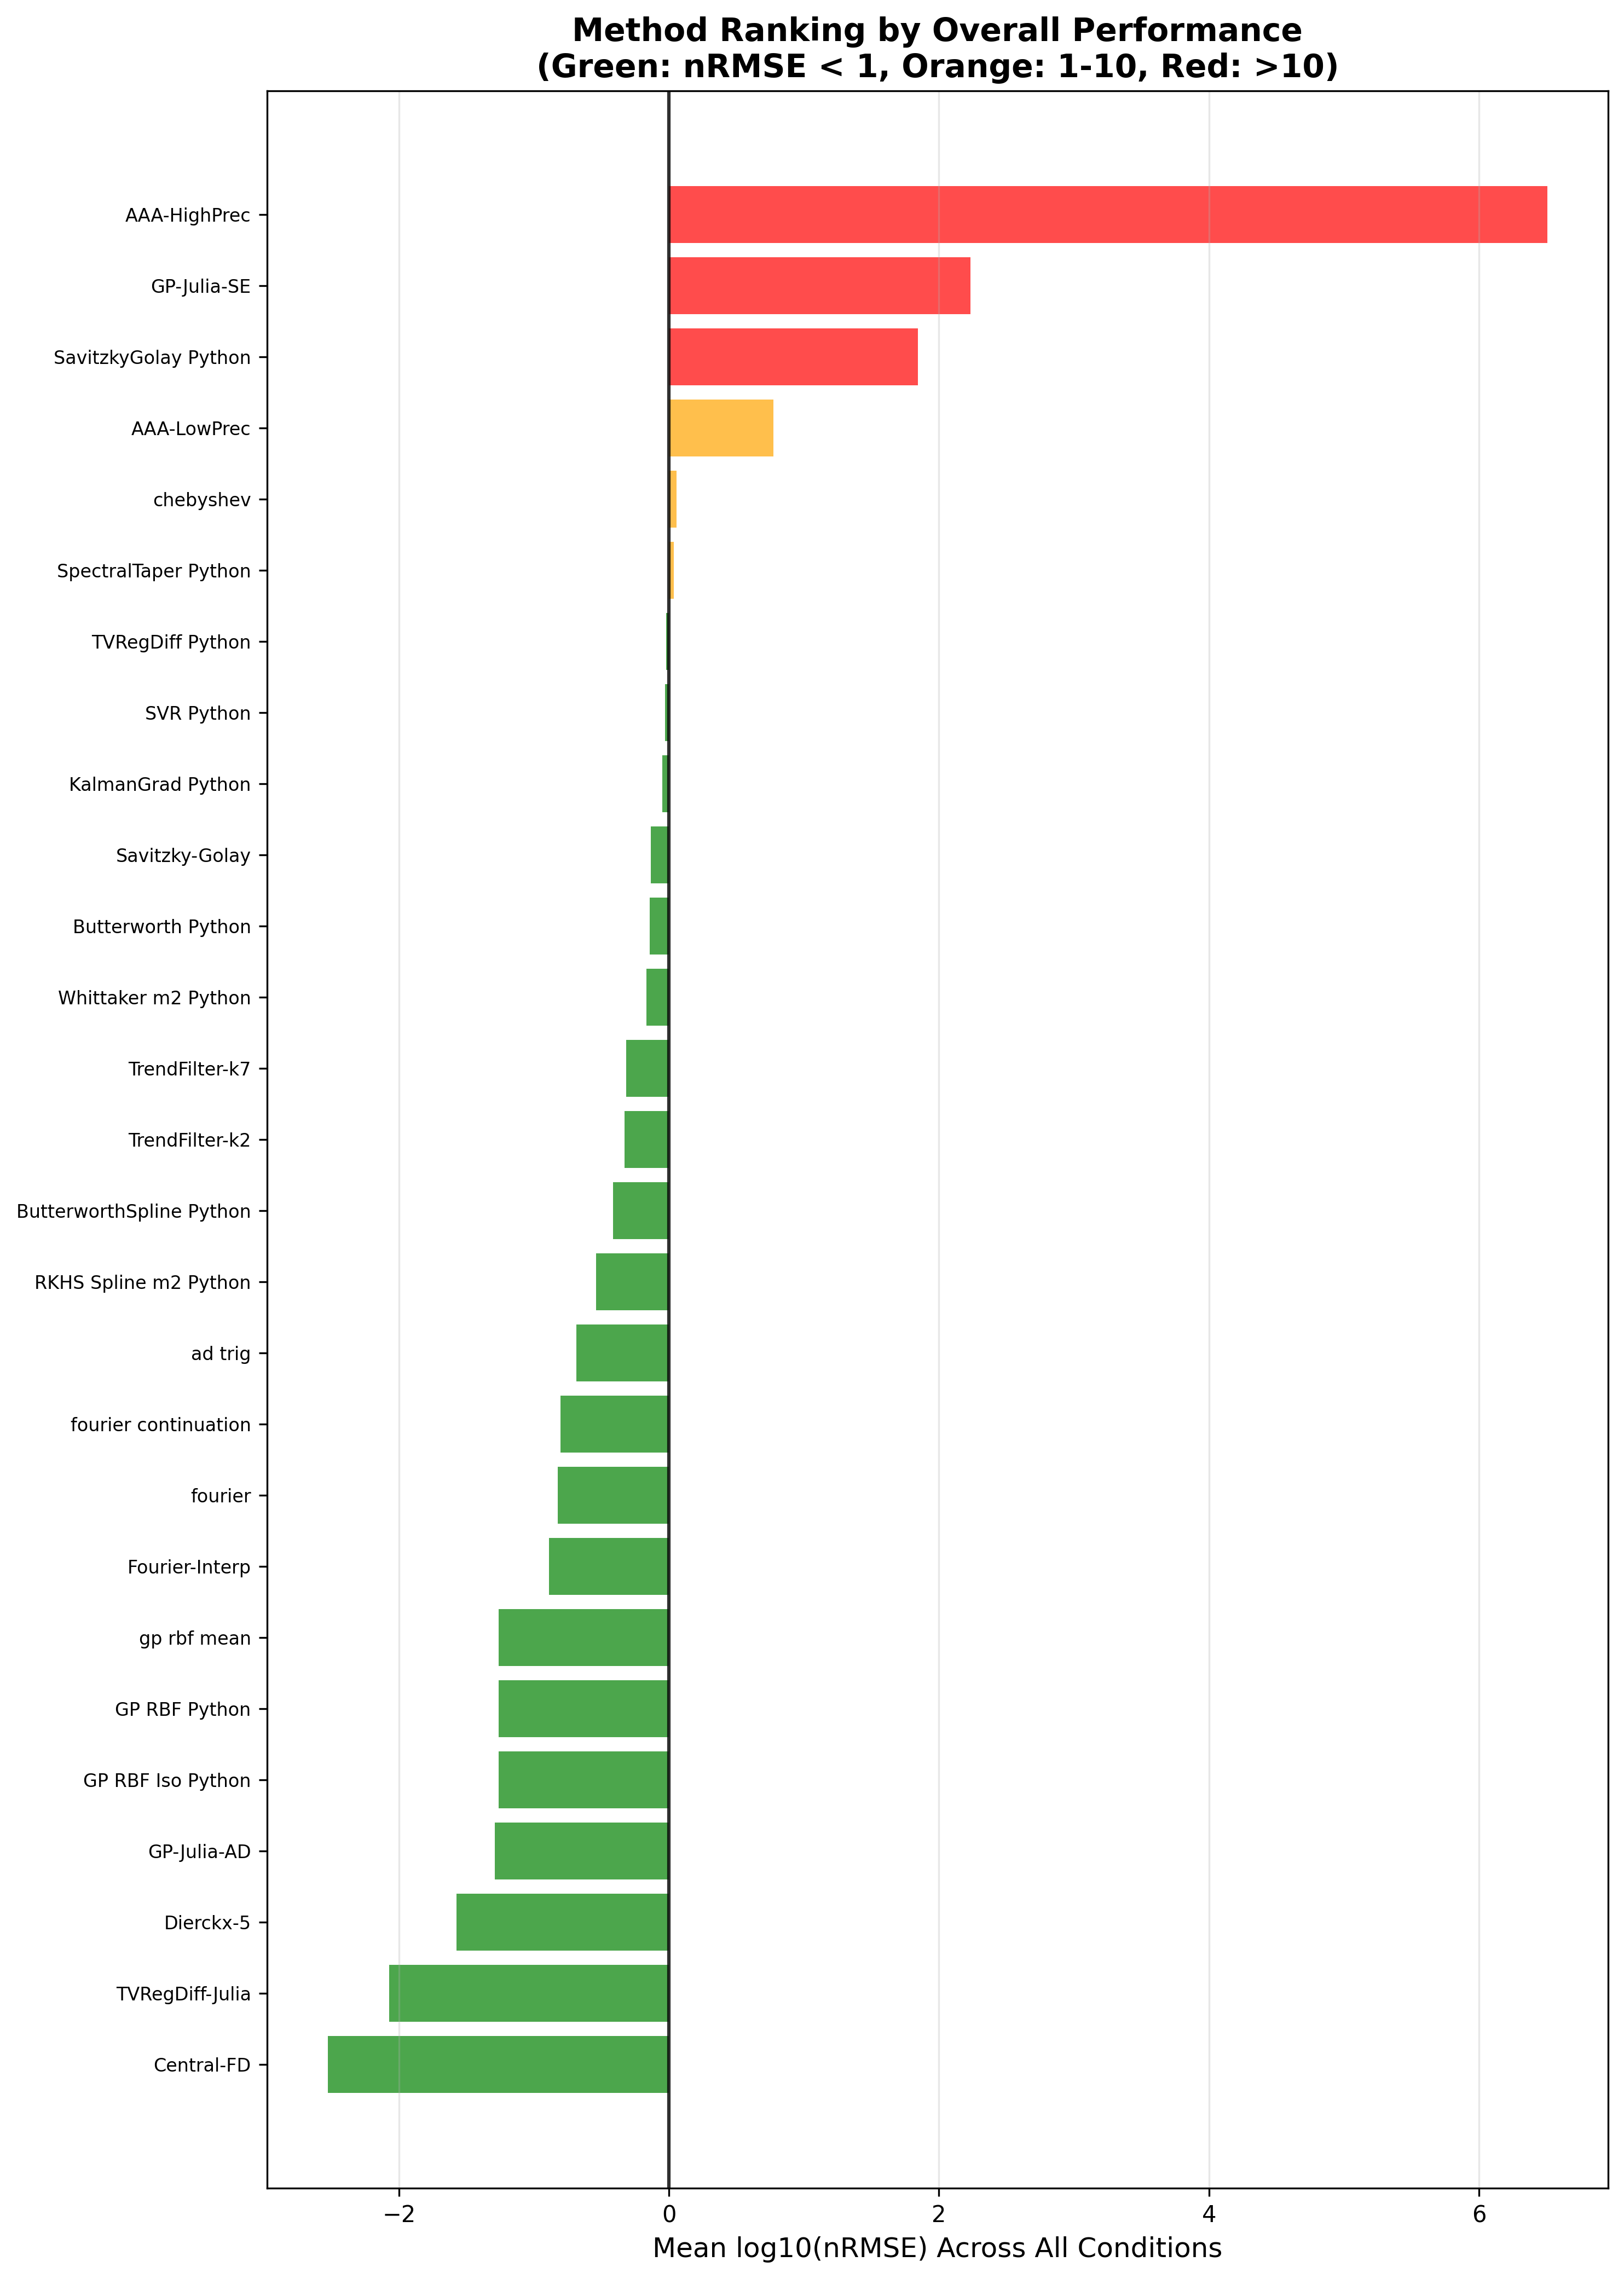
\includegraphics[width=0.85\textwidth]{plot05_ranking_bar_chart.png}
\end{figure}

\clearpage

%==============================================================================
% PLOT 6
%==============================================================================

\section*{Plot 6: Mean vs Std Scatter}

\textbf{What it shows:} Performance consistency (mean vs std of log10(nRMSE)), colored by category

\textbf{Strengths:}
\begin{itemize}
    \item Identifies accurate AND consistent methods
    \item Category colors reveal algorithmic patterns
    \item Lower-left quadrant = ideal methods
    \item Method labels allow identification
\end{itemize}

\textbf{Best for:} Distinguishing reliable methods from variable ones

\begin{figure}[h]
\centering
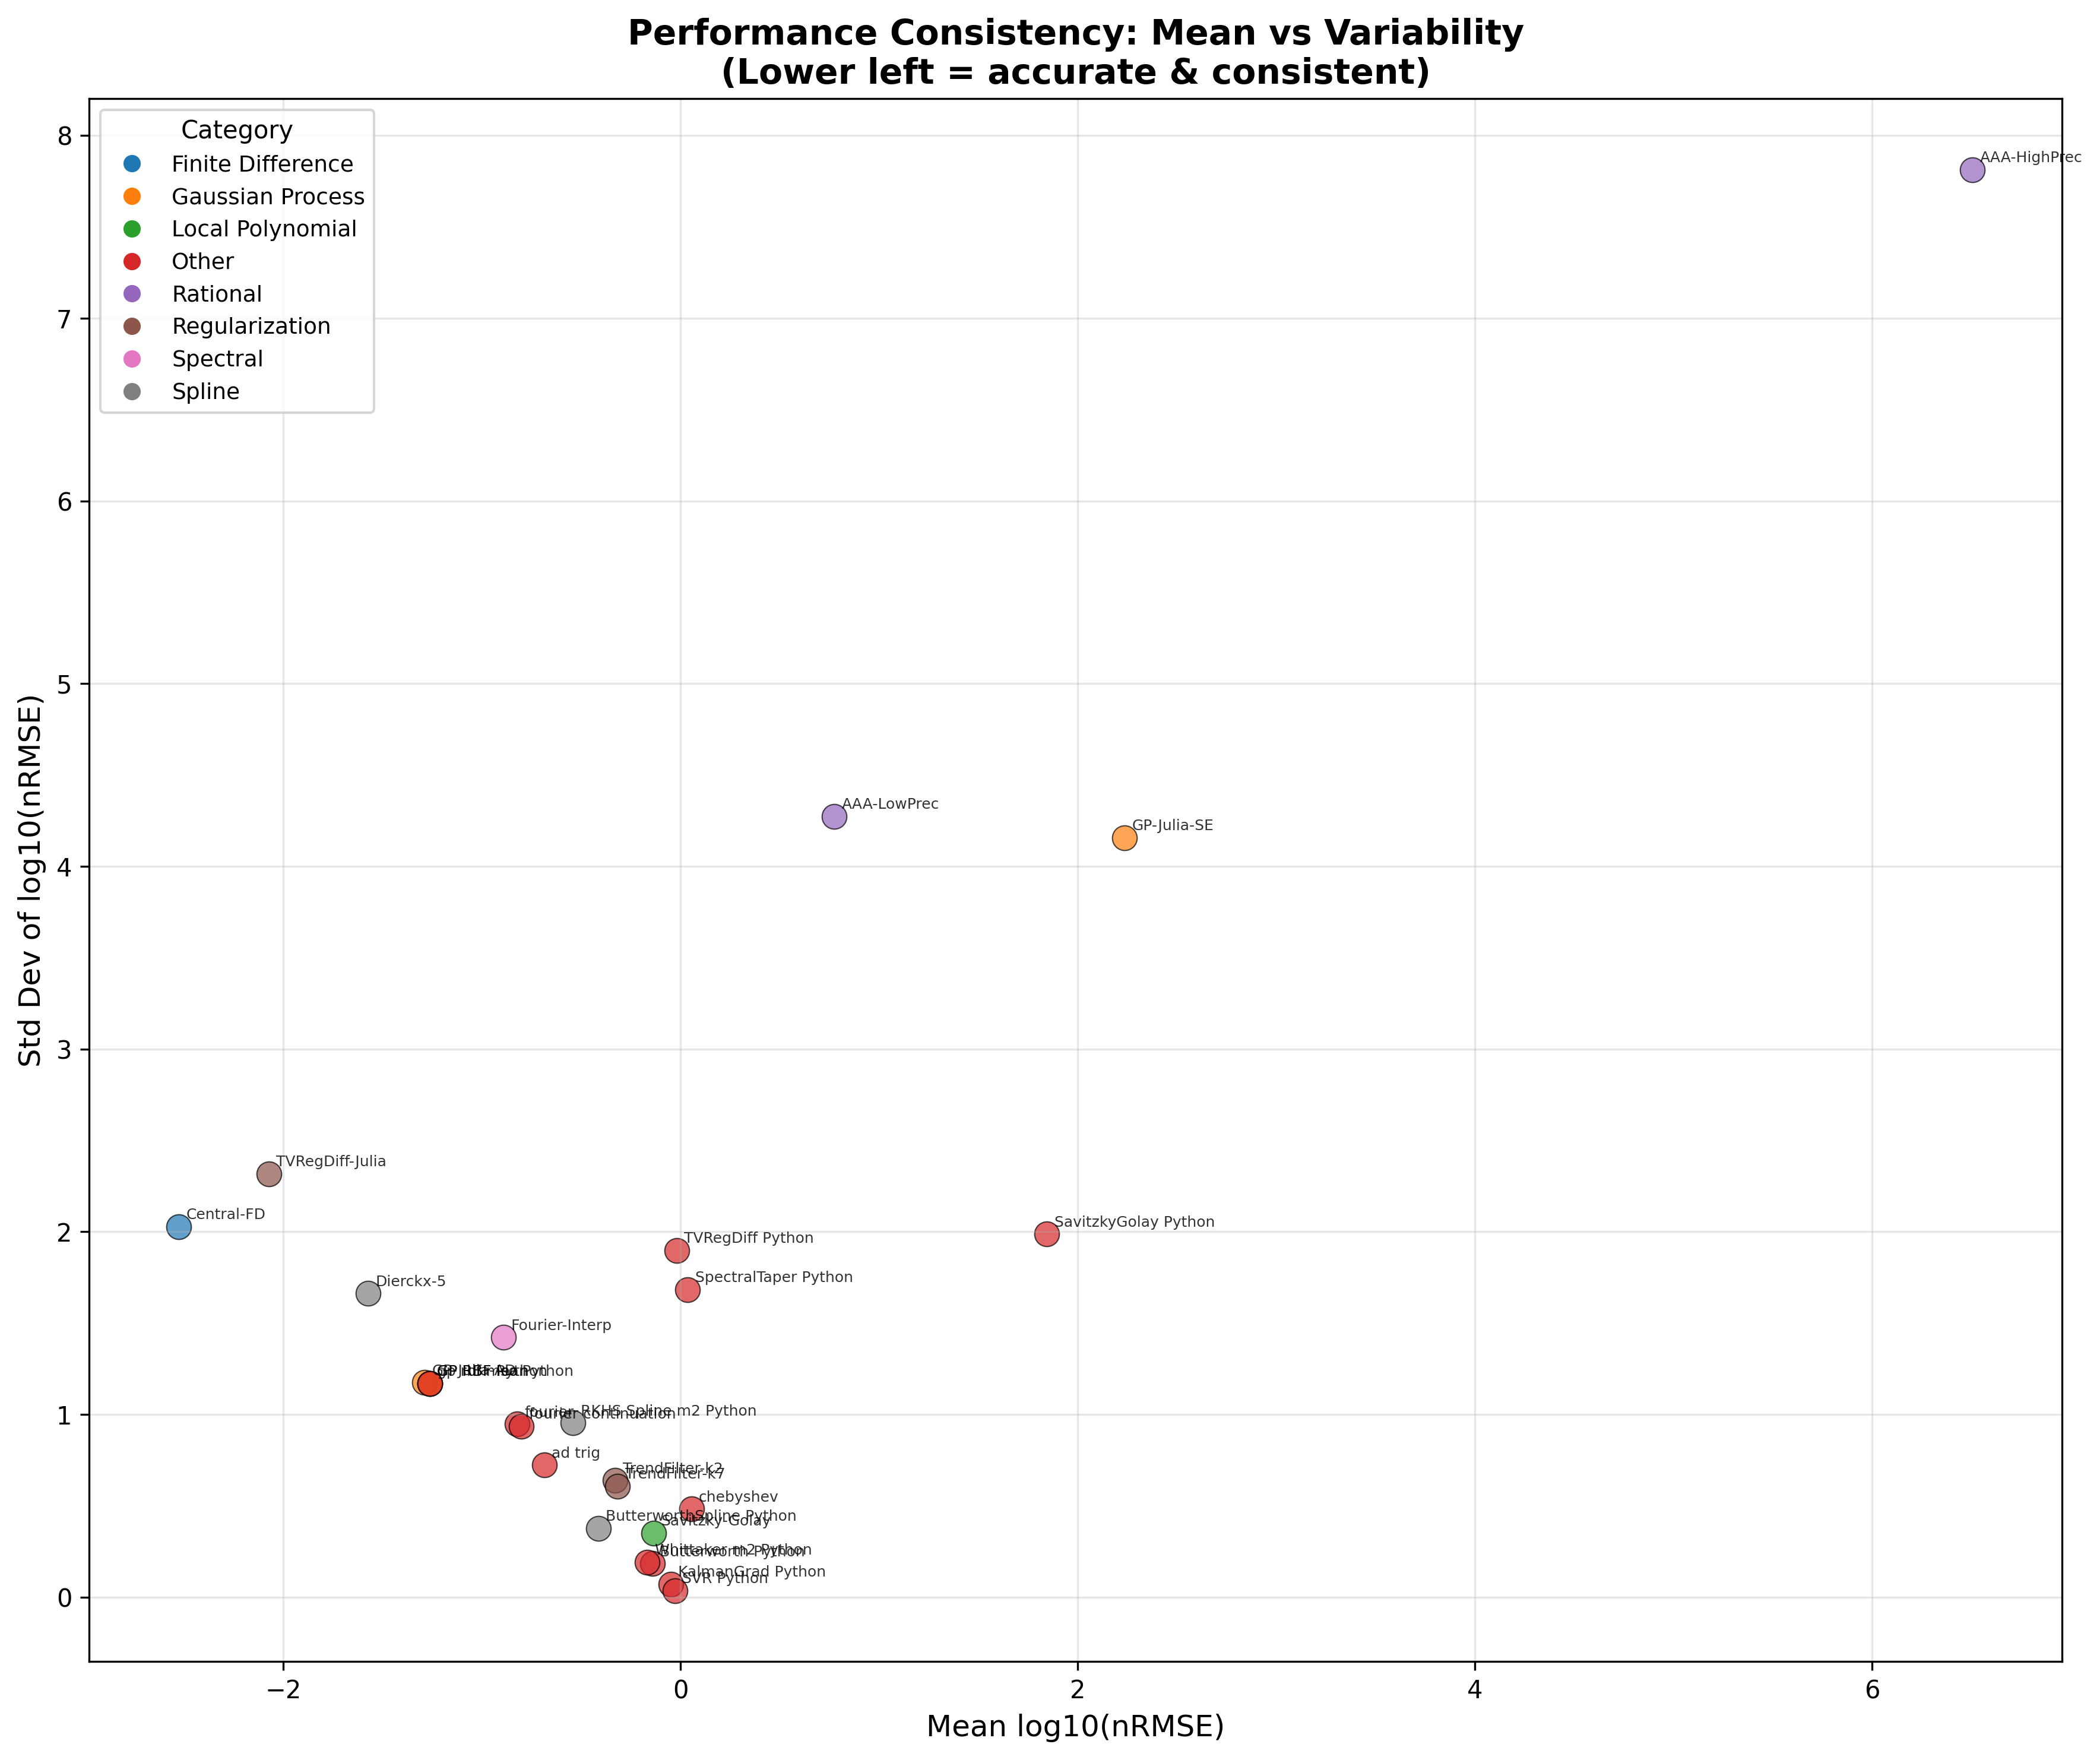
\includegraphics[width=\textwidth]{plot06_scatter_mean_std.png}
\end{figure}

\clearpage

%==============================================================================
% PLOT 7
%==============================================================================

\section*{Plot 7: Failure Rate Analysis}

\textbf{What it shows:} Percentage of conditions where each method has nRMSE $>$ 10

\textbf{Strengths:}
\begin{itemize}
    \item Directly quantifies reliability
    \item Highlights methods prone to catastrophic failures
    \item Color-coded by severity
    \item Complements average performance metrics
\end{itemize}

\textbf{Best for:} Risk assessment, supporting ``avoid AAA for orders $\geq 3$'' recommendation

\begin{figure}[h]
\centering
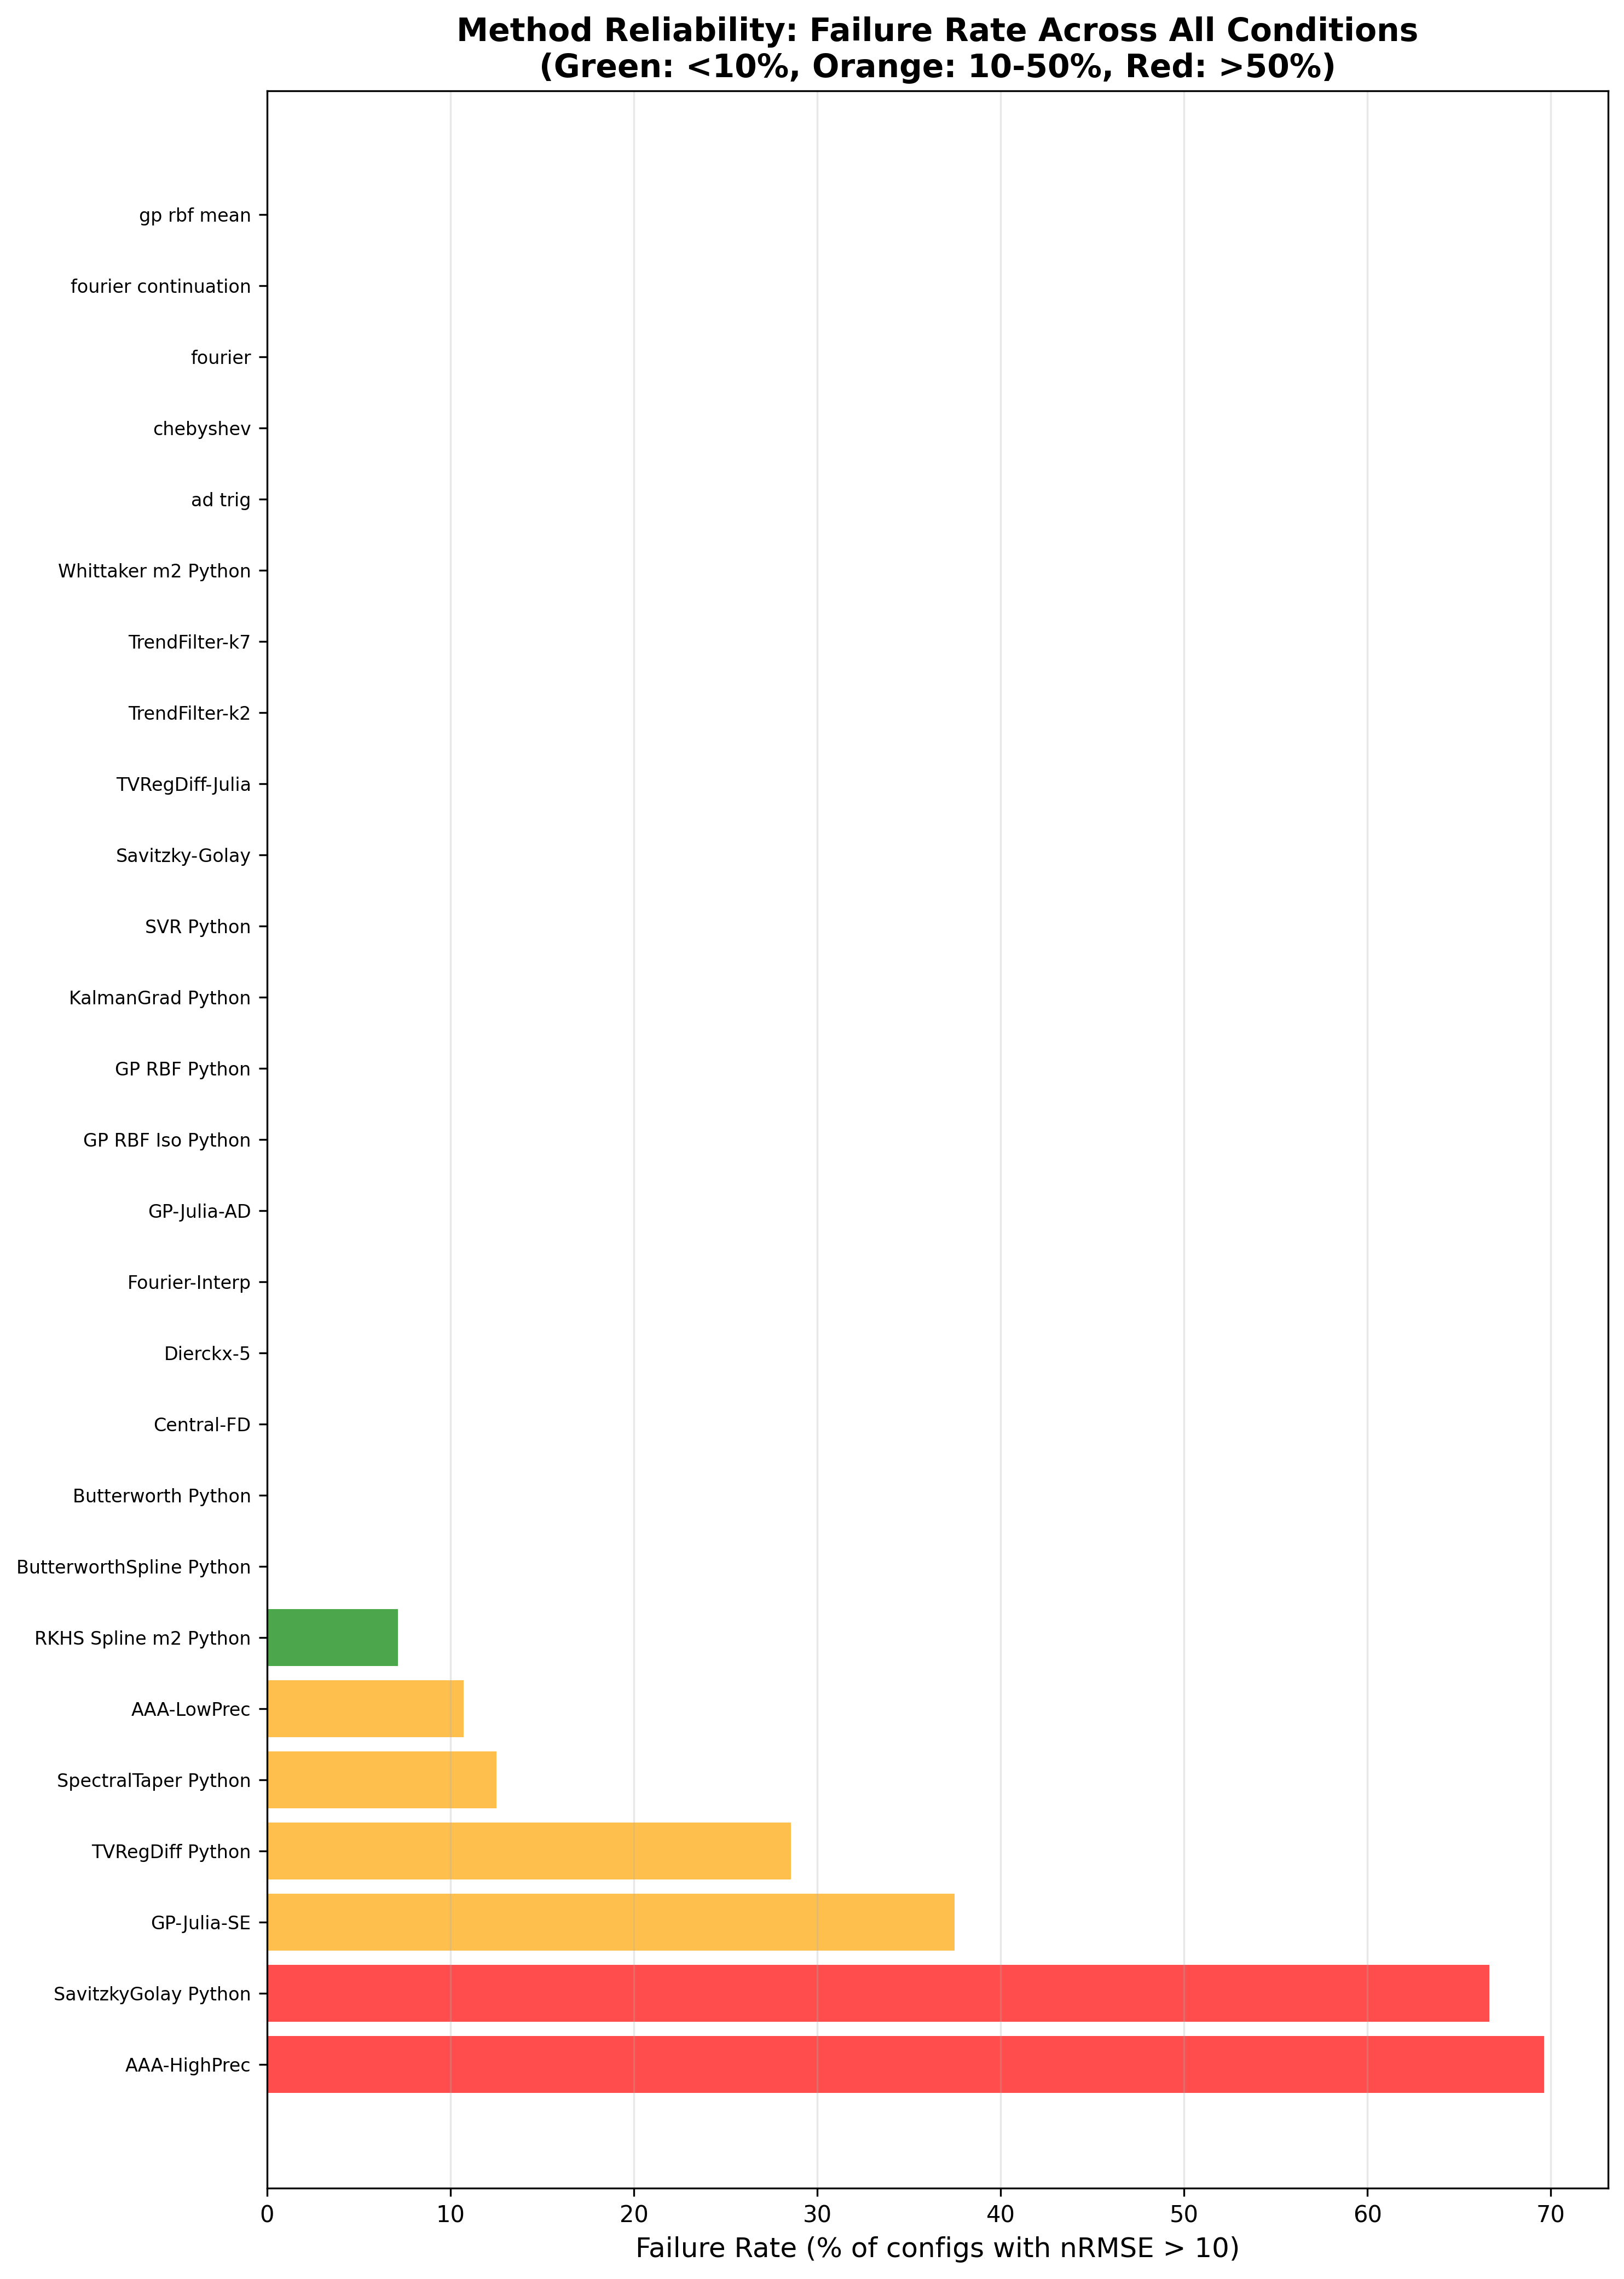
\includegraphics[width=0.85\textwidth]{plot07_failure_rate.png}
\end{figure}

\clearpage

%==============================================================================
% PLOT 8
%==============================================================================

\section*{Plot 8: Category Box Plots}

\textbf{What it shows:} Performance distribution by method category (GP, Rational, Spectral, etc.)

\textbf{Strengths:}
\begin{itemize}
    \item Shows algorithmic approach strengths/weaknesses
    \item Box plots reveal full distribution (not just mean)
    \item Supports ``GP methods excel'' narrative
    \item Fewer boxes = easier to read than per-method plots
\end{itemize}

\textbf{Best for:} High-level category comparison, algorithm selection guidance

\begin{figure}[h]
\centering
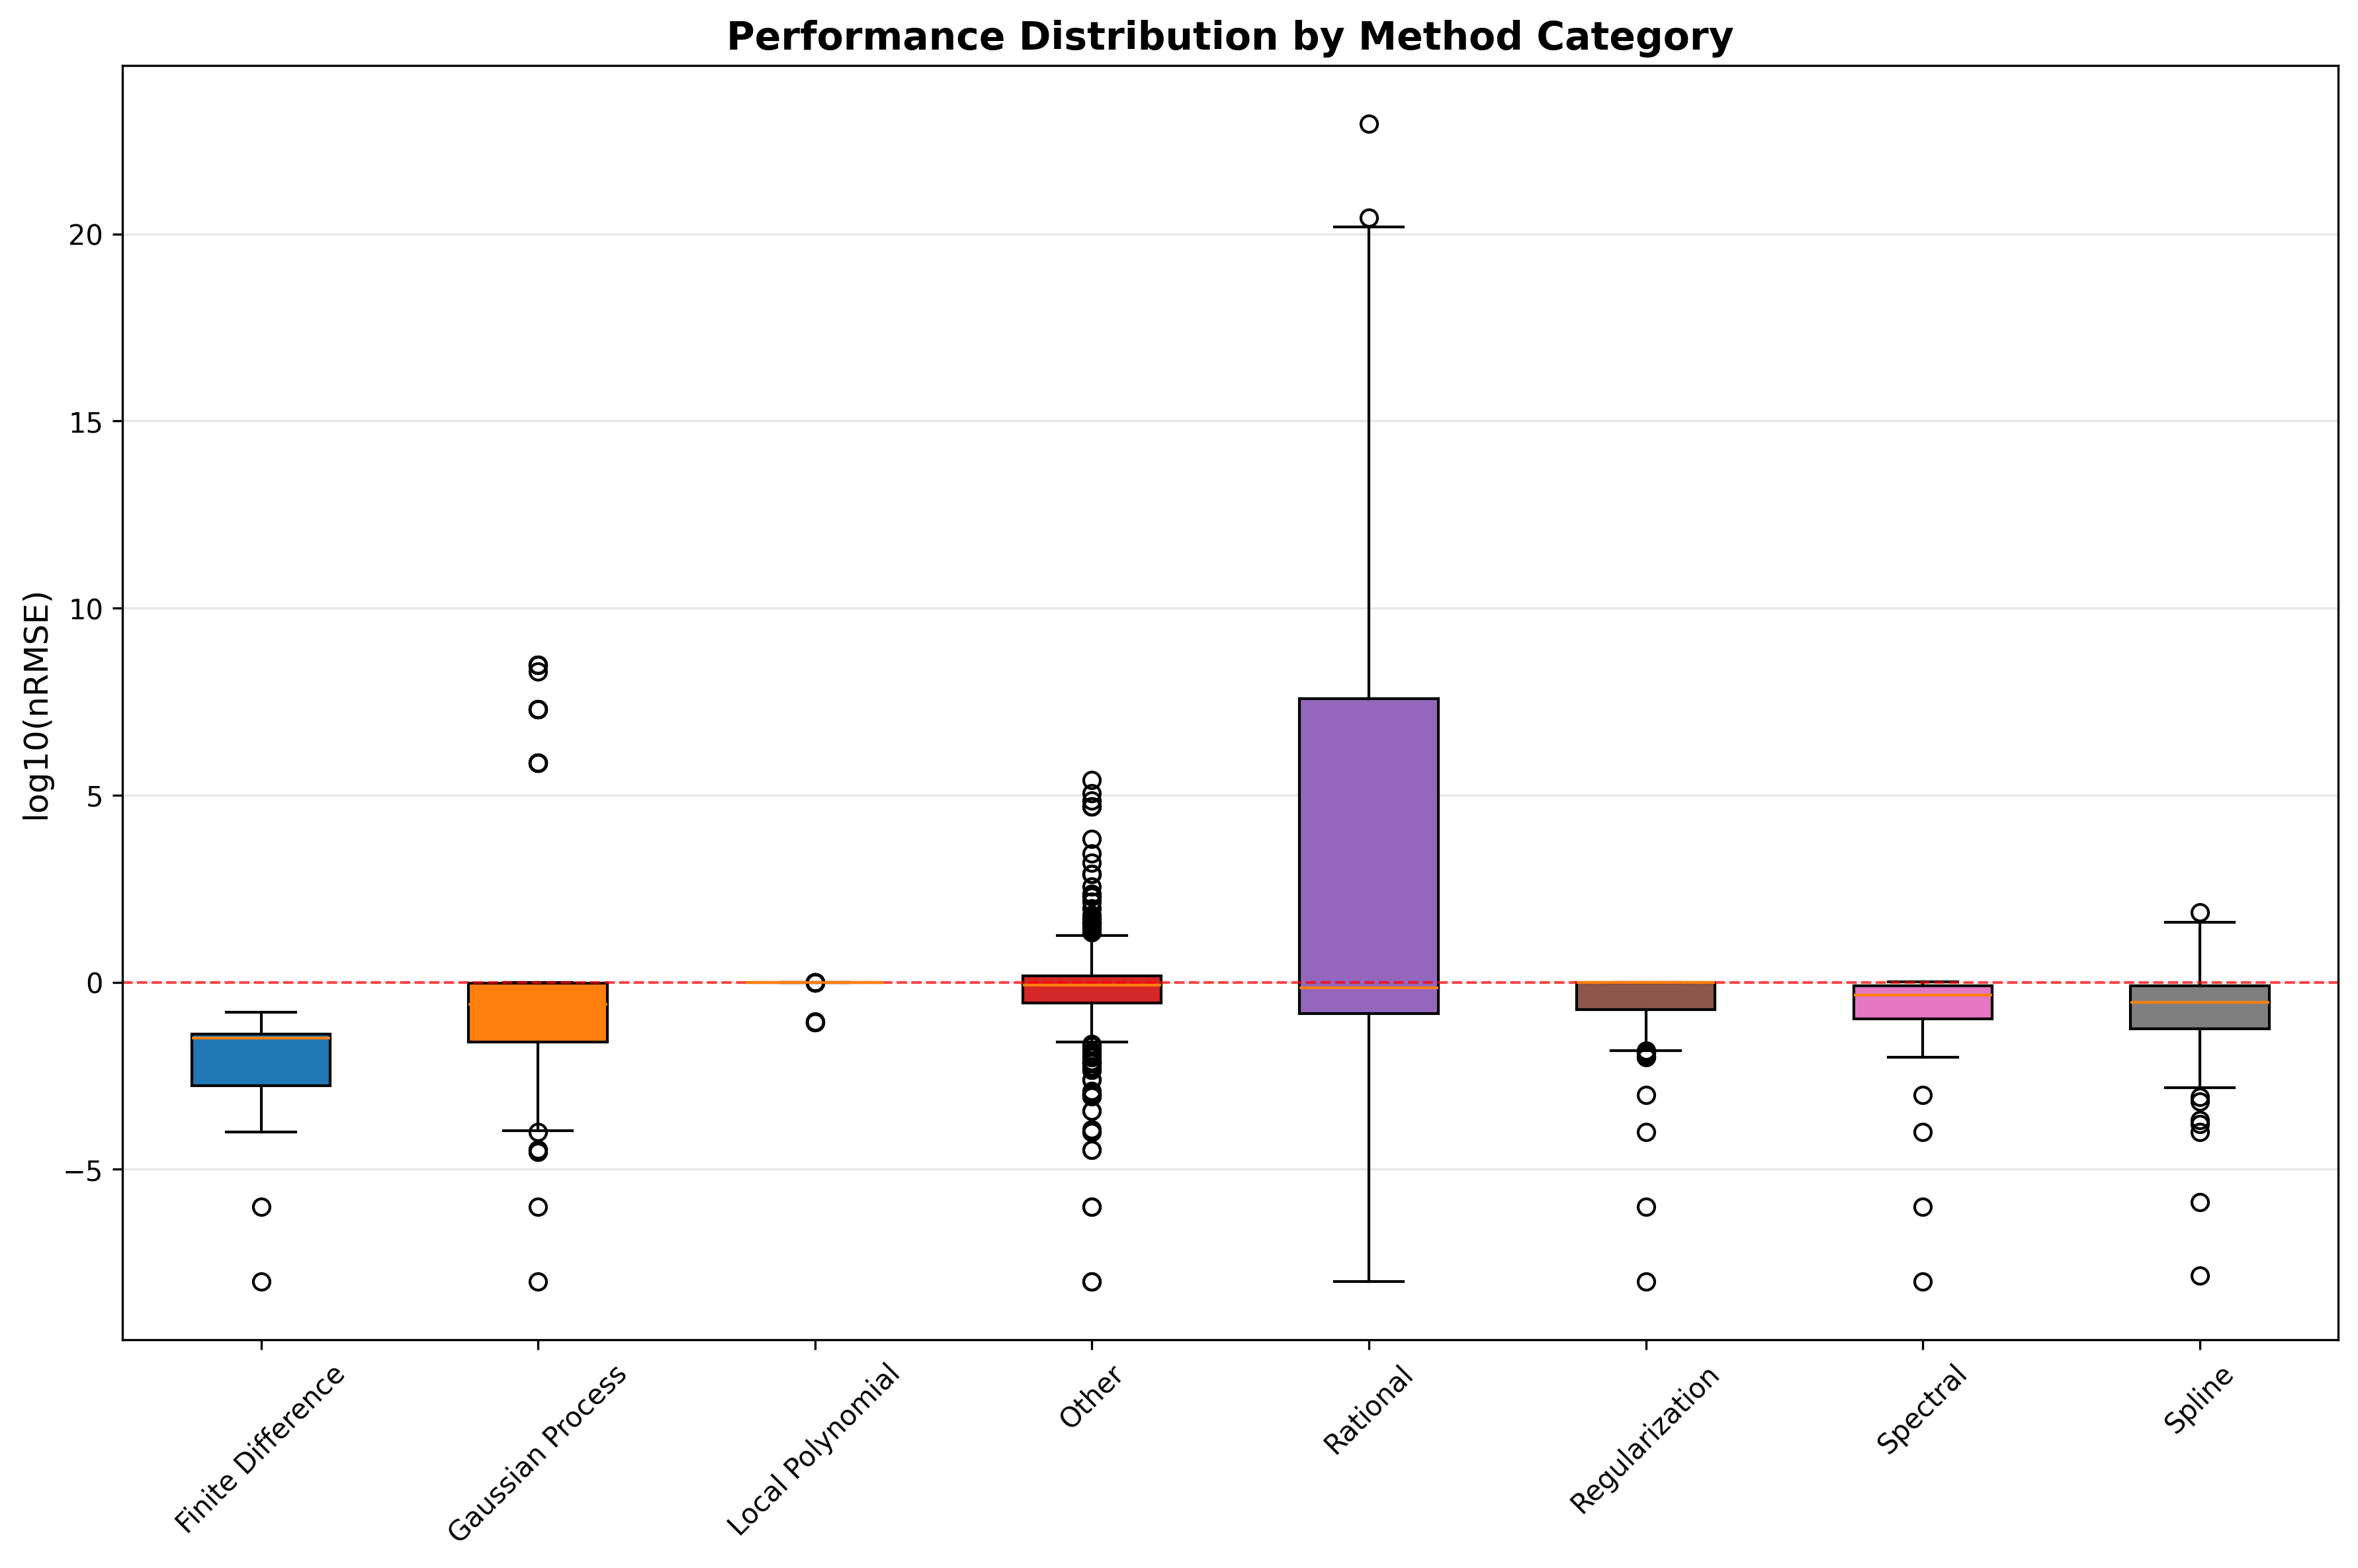
\includegraphics[width=\textwidth]{plot08_category_boxplot.png}
\end{figure}

\clearpage

%==============================================================================
% PLOT 9
%==============================================================================

\section*{Plot 9: Category Trends vs Order}

\textbf{What it shows:} How each category's average performance degrades with derivative order

\textbf{Strengths:}
\begin{itemize}
    \item Reveals category-level order sensitivity
    \item Simpler than per-method line plots (6 lines vs 16+)
    \item Shows which approaches scale better to high orders
    \item Clear color coding by category
\end{itemize}

\textbf{Best for:} Algorithm type comparison, predicting behavior at untested orders

\begin{figure}[h]
\centering
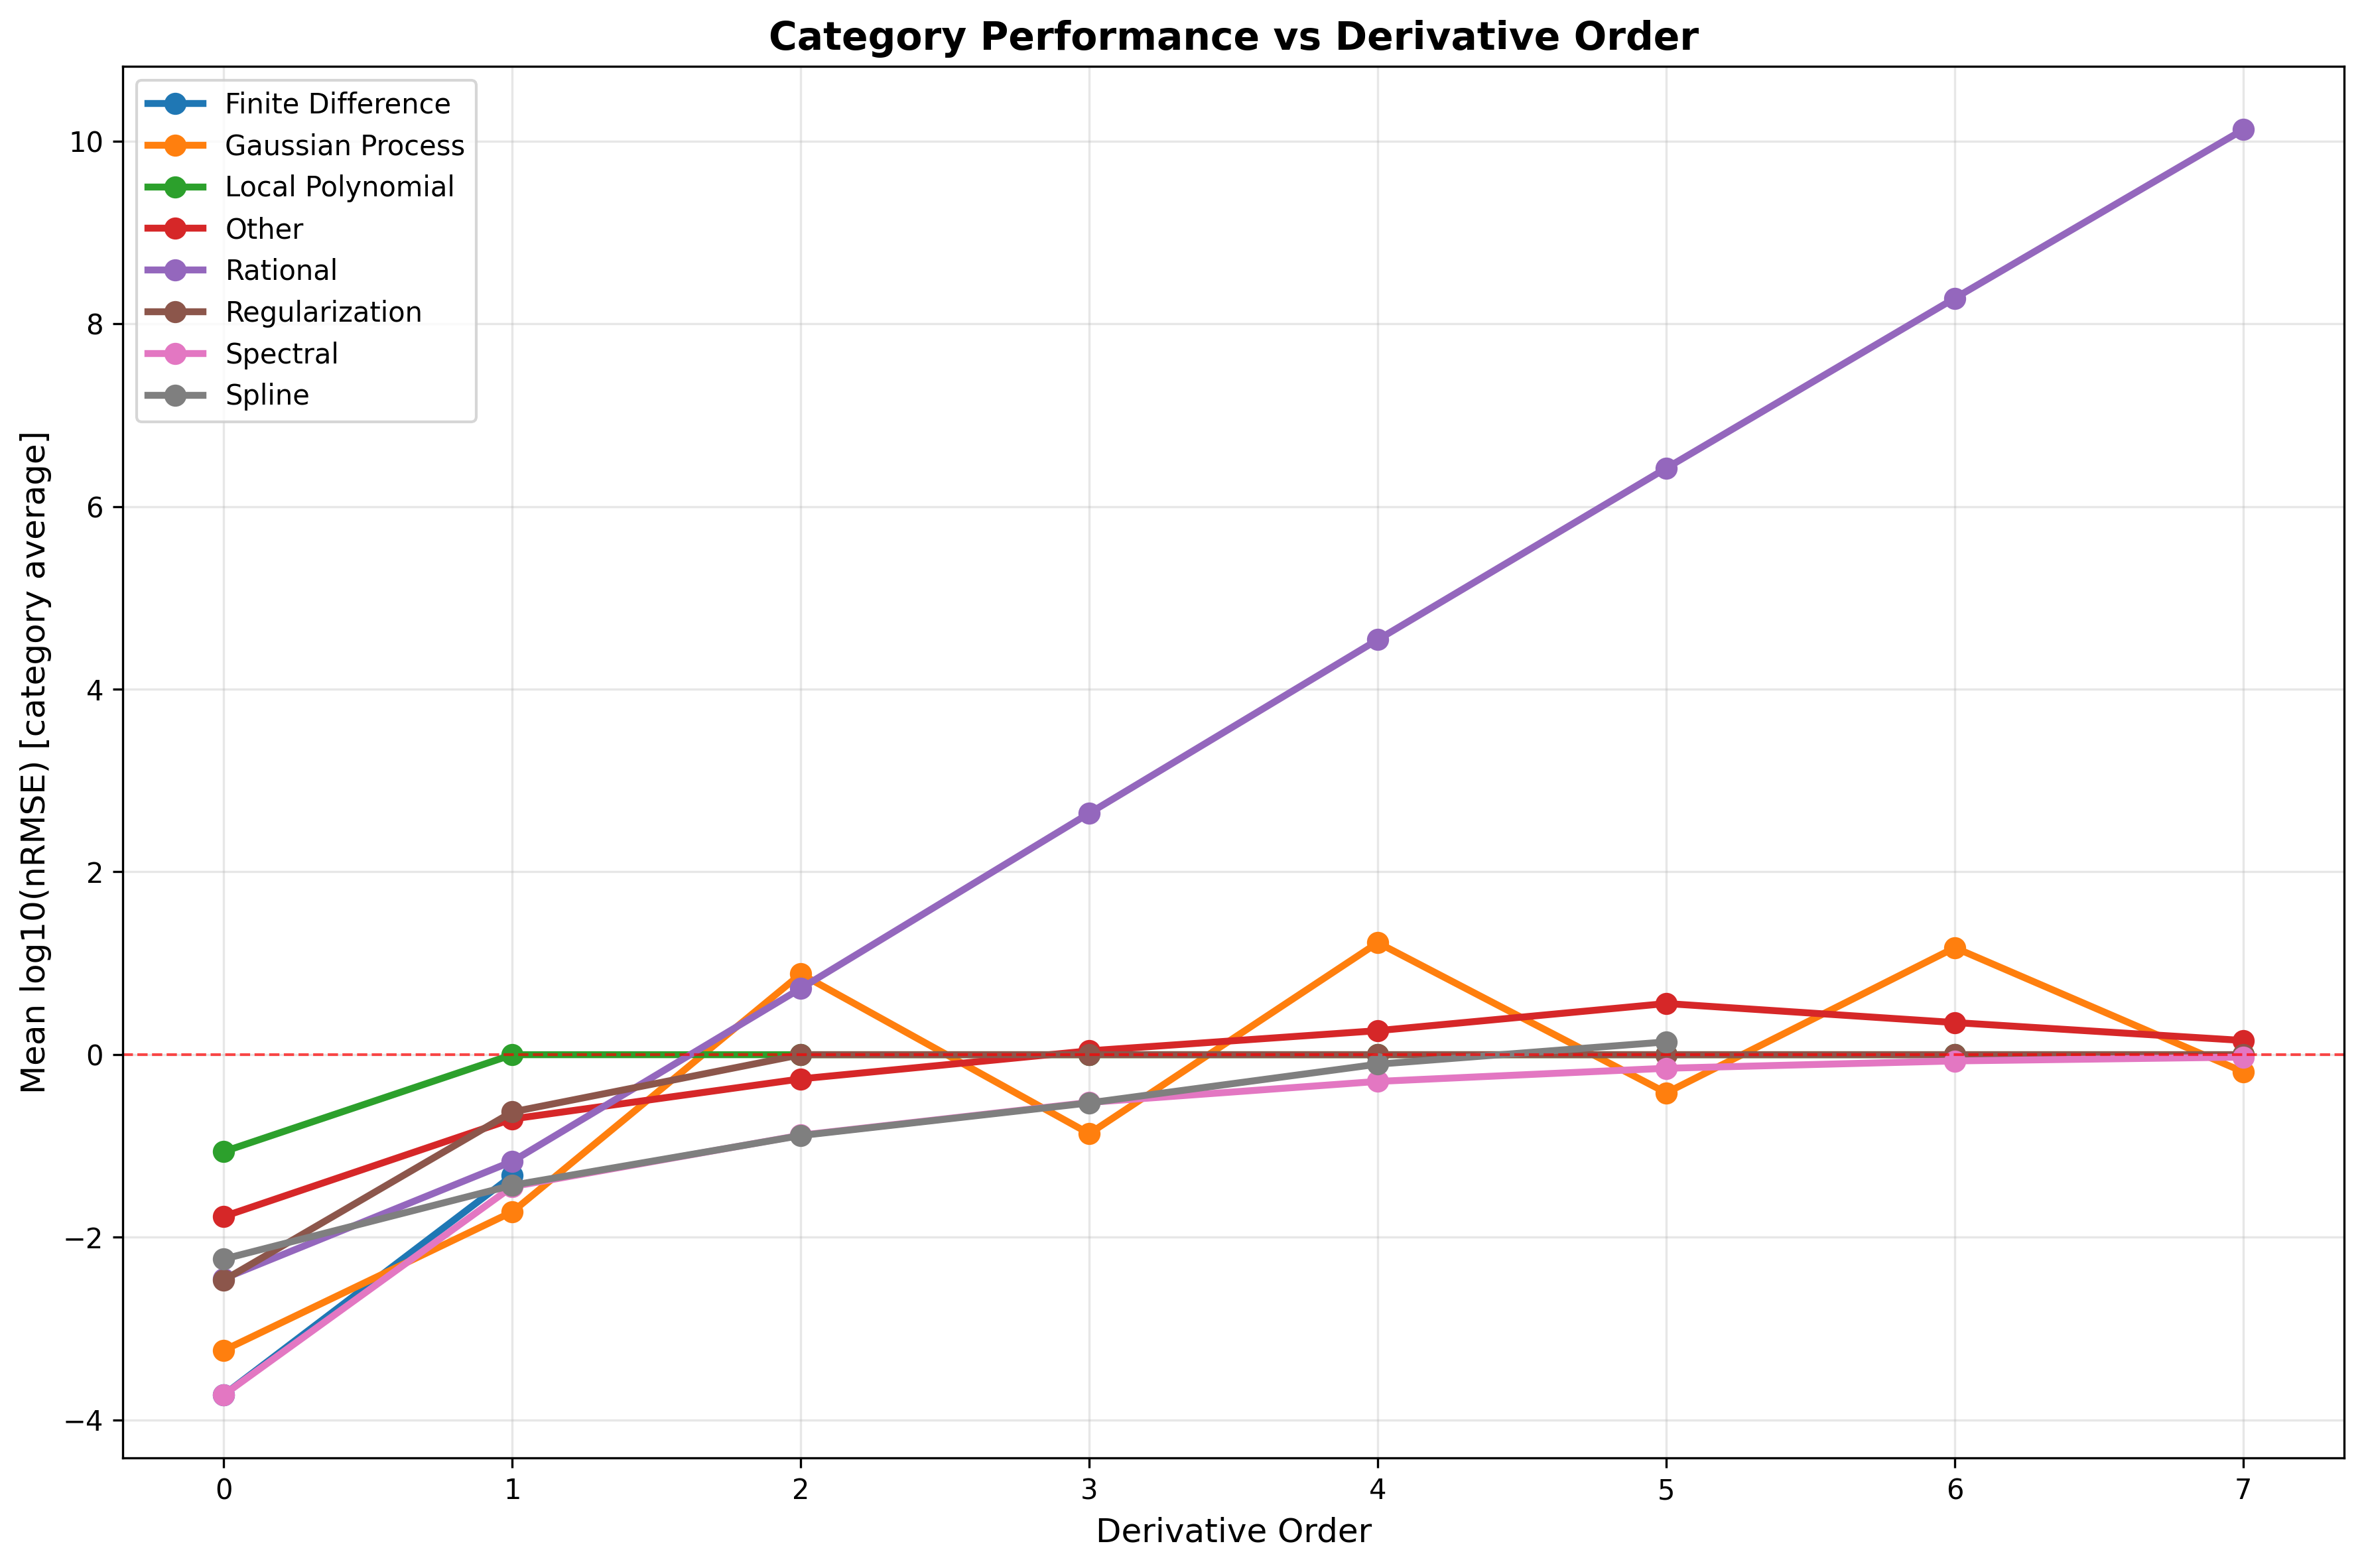
\includegraphics[width=\textwidth]{plot09_category_vs_order.png}
\end{figure}

\clearpage

%==============================================================================
% PLOT 10
%==============================================================================

\section*{Plot 10: Best Method Per Condition Grid}

\textbf{What it shows:} Which method achieves lowest nRMSE for each (order, noise) combination

\textbf{Strengths:}
\begin{itemize}
    \item Practical method selection tool
    \item Shows context-dependent ``best'' method
    \item Reveals GP dominance across most conditions
    \item Text labels allow exact method identification
\end{itemize}

\textbf{Best for:} Method selection by application requirements, lookup table for practitioners

\begin{figure}[h]
\centering
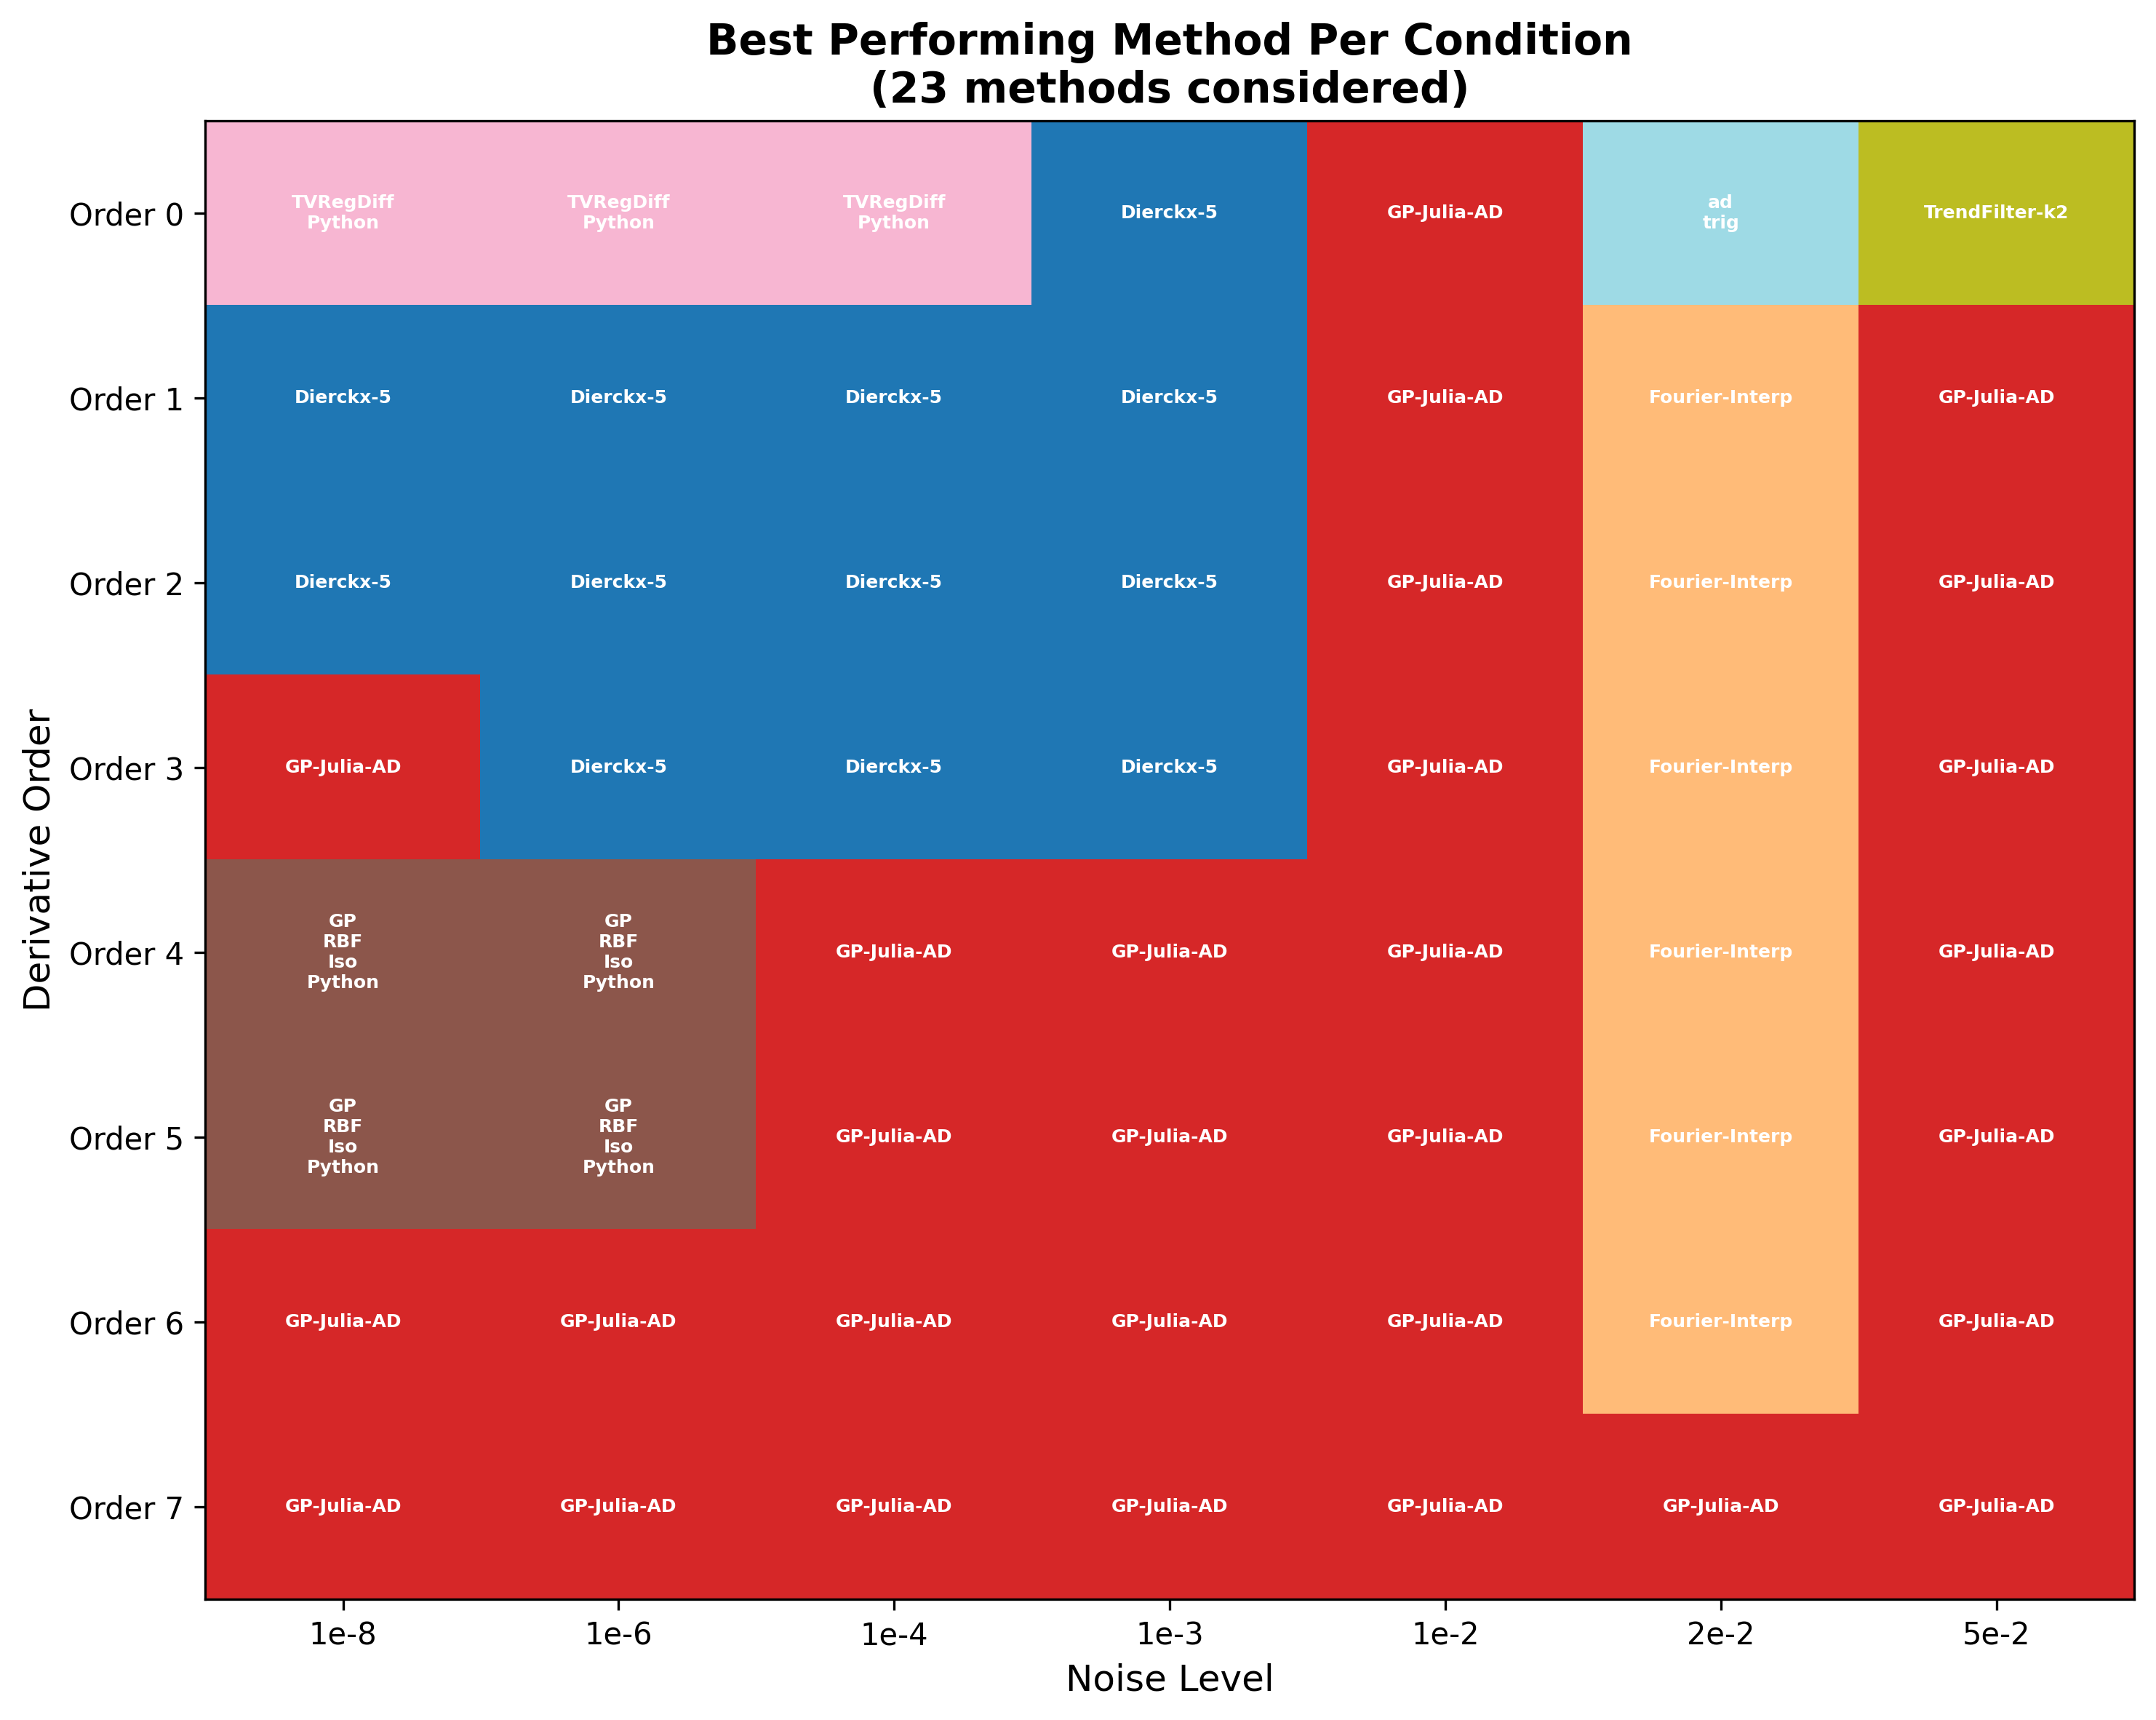
\includegraphics[width=0.85\textwidth]{plot10_best_method_grid.png}
\end{figure}

\clearpage

%==============================================================================
% PLOT 11
%==============================================================================

\section*{Plot 11: Stacked Performance Categories}

\textbf{What it shows:} Percentage of conditions falling into performance bins (Excellent/Good/Acceptable/Failed)

\textbf{Strengths:}
\begin{itemize}
    \item Balanced view of successes and failures
    \item Easy to see ``all-around'' methods (mostly green/yellow)
    \item Highlights fragile methods (large red sections)
    \item Sorted by ``excellent'' percentage
\end{itemize}

\textbf{Best for:} Qualitative performance summary, reliability visualization

\begin{figure}[h]
\centering
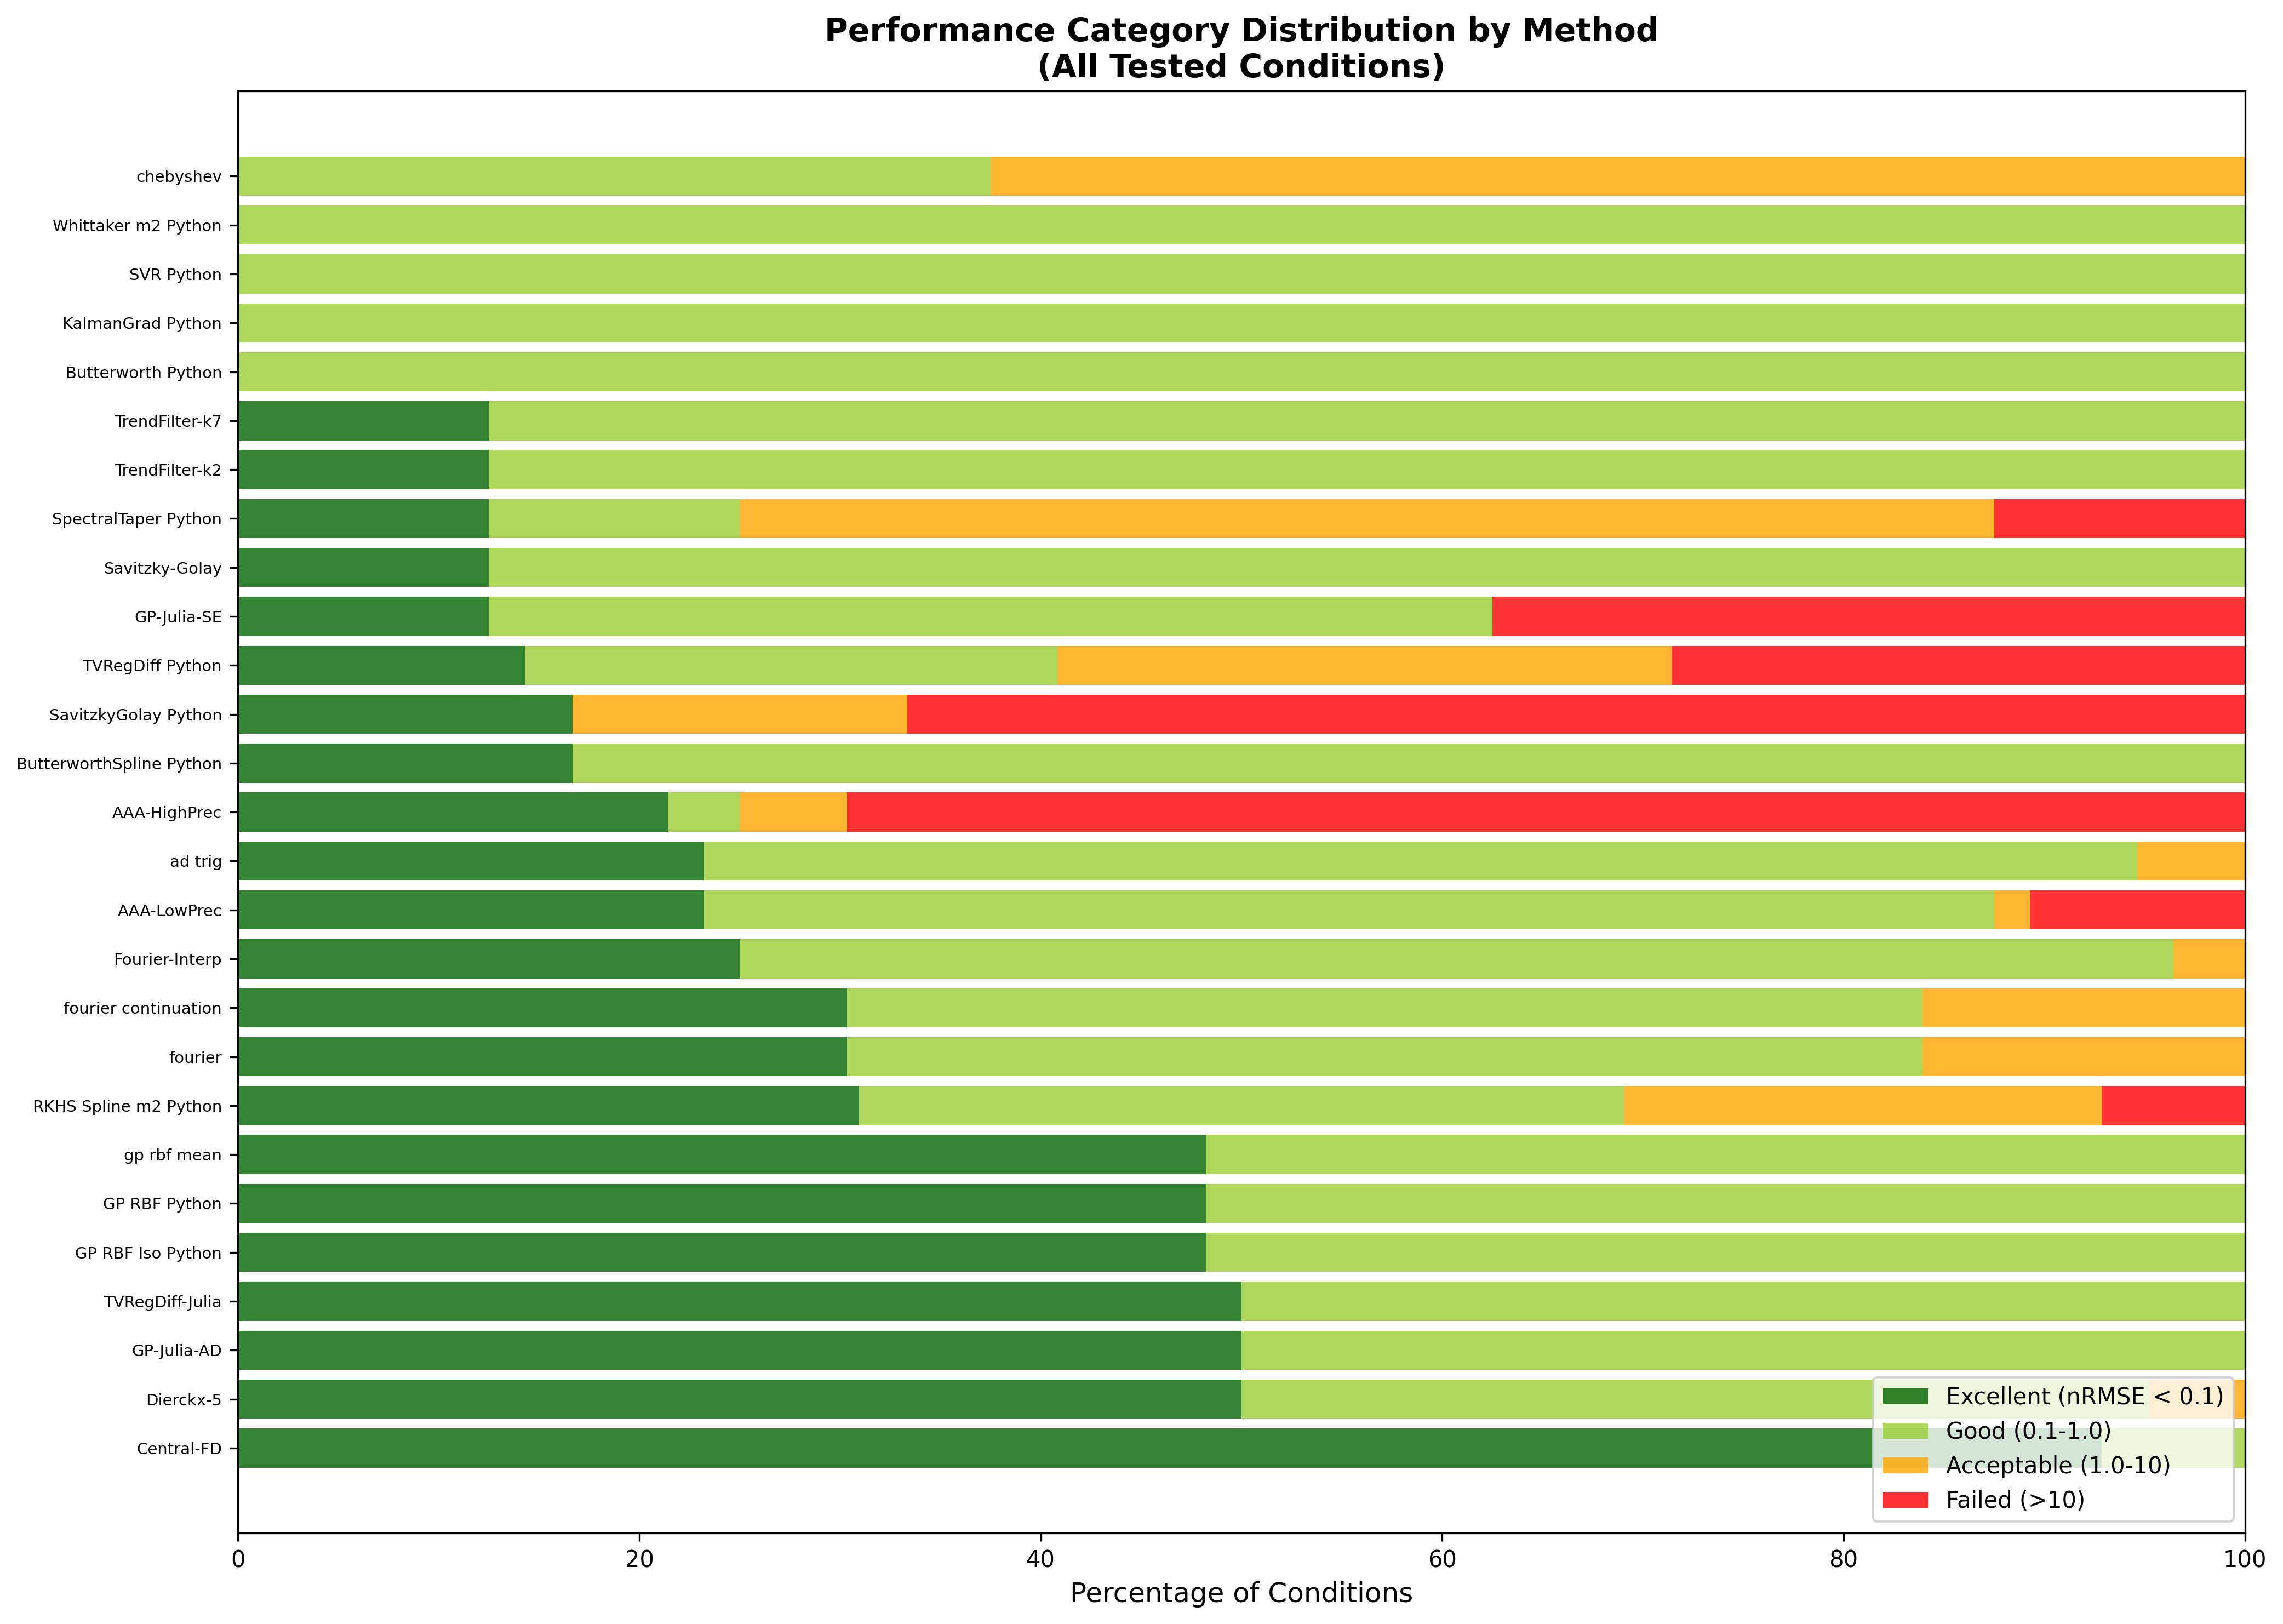
\includegraphics[width=\textwidth]{plot11_stacked_performance.png}
\end{figure}

\clearpage

%==============================================================================
% PLOT 12
%==============================================================================

\section*{Plot 12: Performance Relative to Baseline}

\textbf{What it shows:} log10(method nRMSE / GP-Julia-AD nRMSE) for selected methods

\textbf{Strengths:}
\begin{itemize}
    \item Direct comparison to top performer
    \item Values $>$ 0 mean worse, $<$ 0 mean better
    \item Shows which methods can beat GP in specific conditions
    \item 8-panel layout shows order-specific patterns
\end{itemize}

\textbf{Best for:} Relative performance assessment, identifying niche strengths

\begin{figure}[h]
\centering
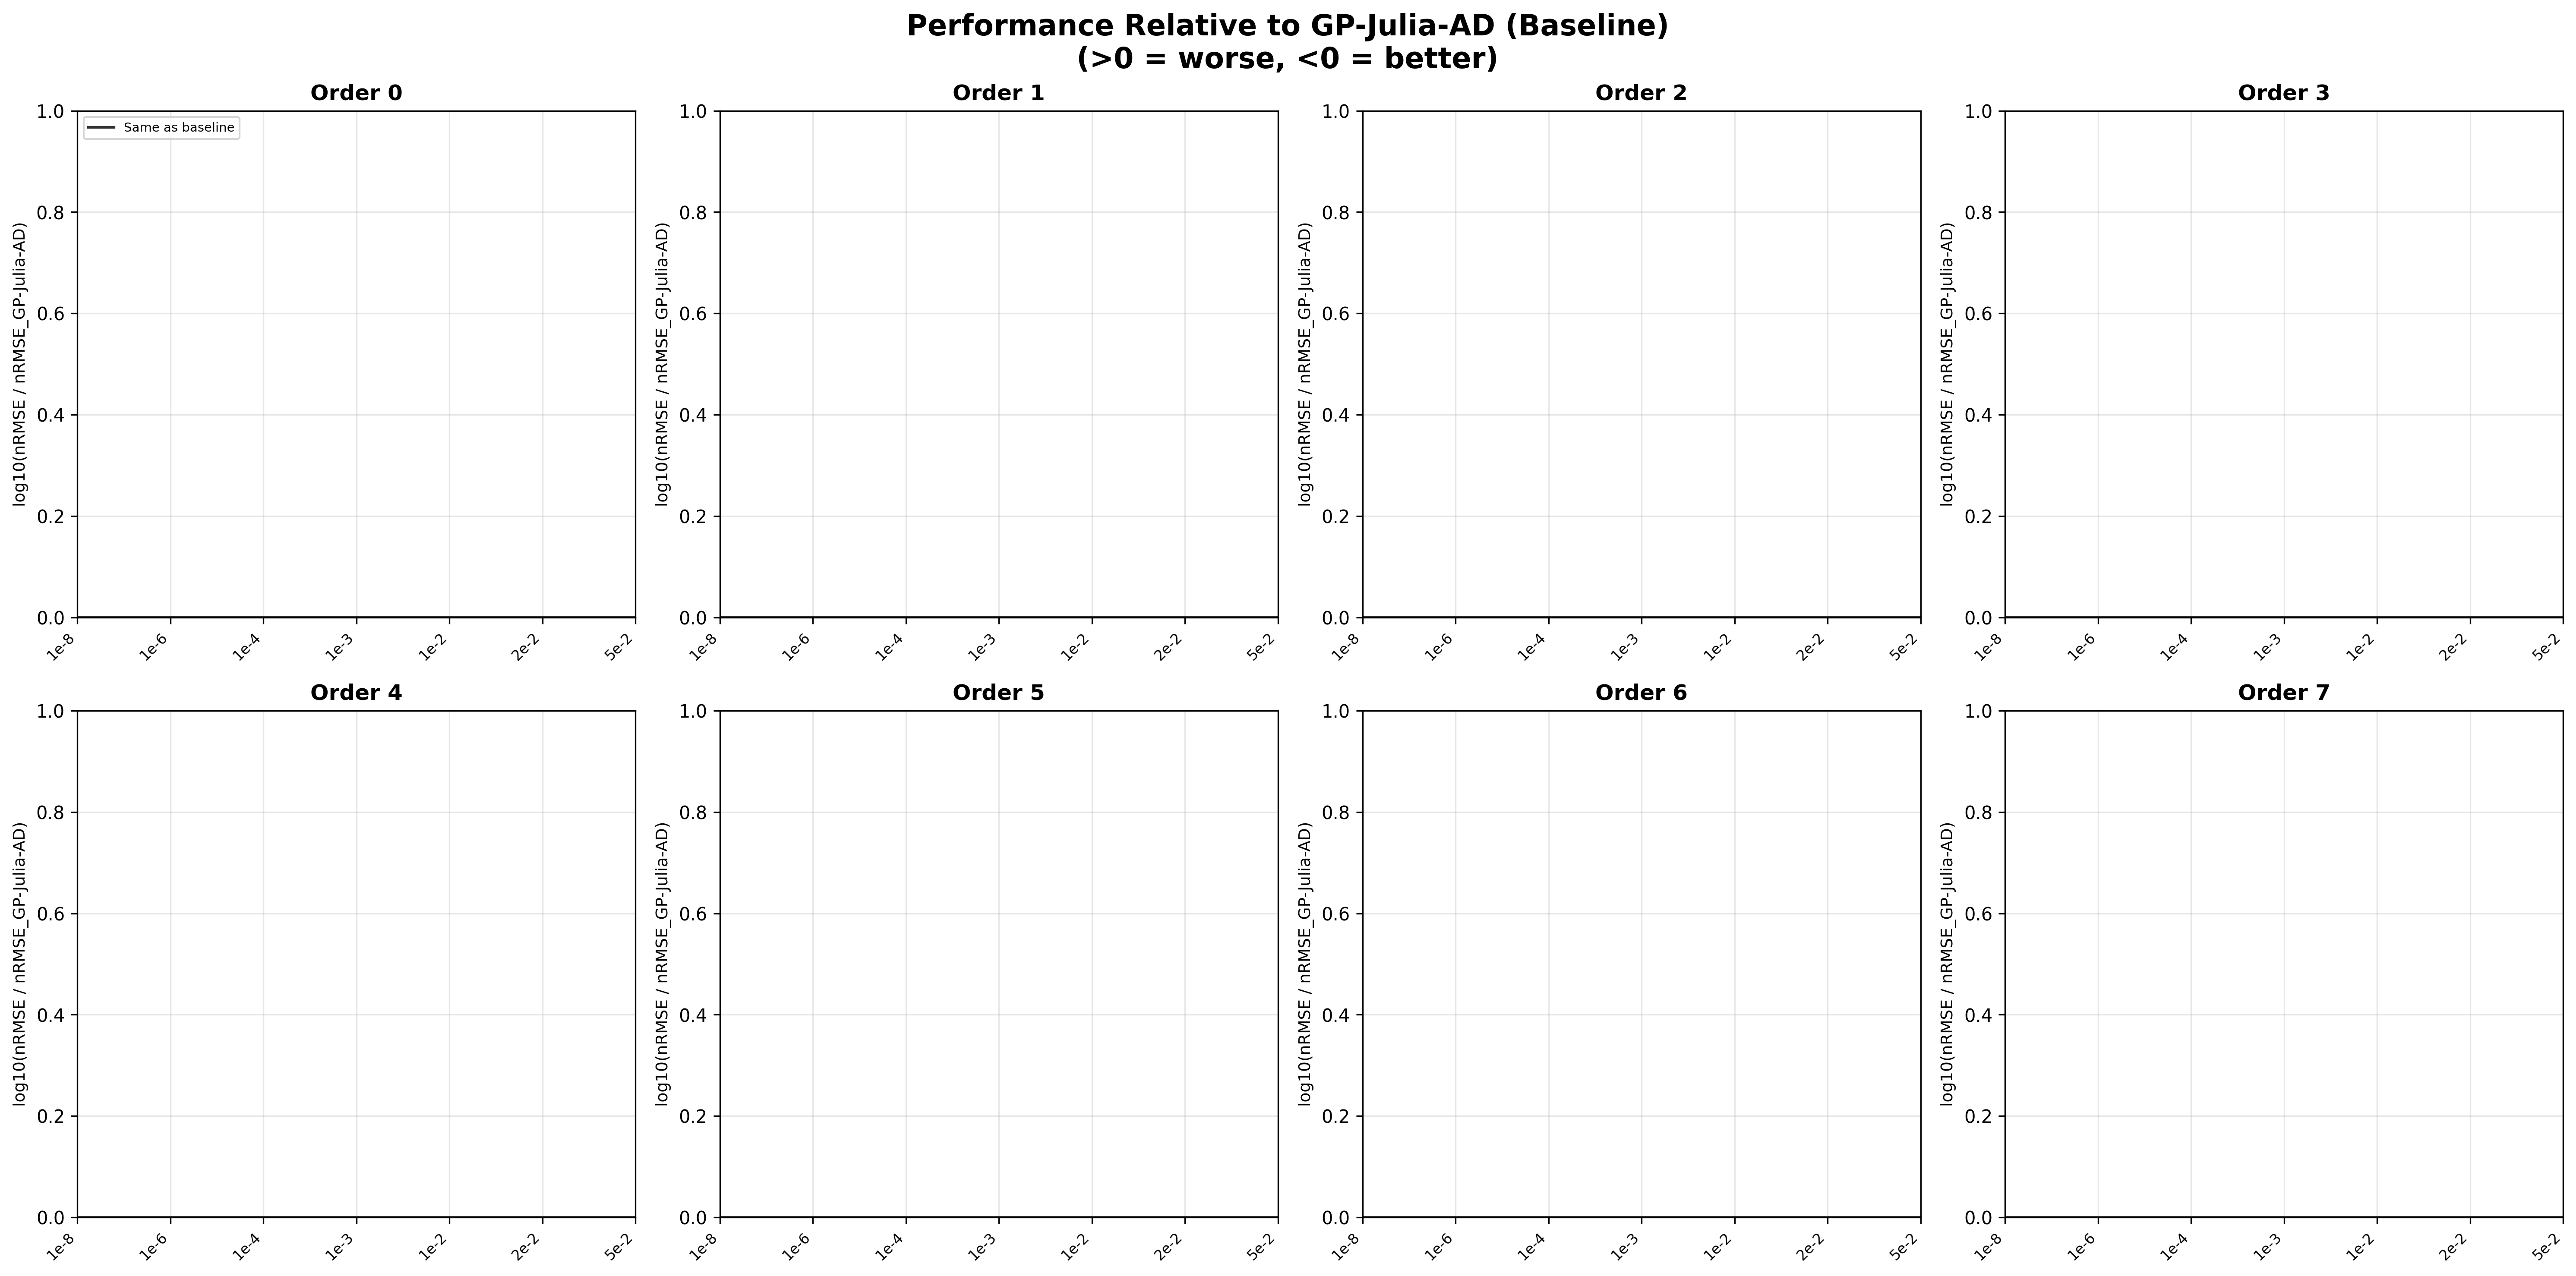
\includegraphics[width=\textwidth]{plot12_vs_baseline.png}
\end{figure}

\clearpage

%==============================================================================
% PLOT 13
%==============================================================================

\section*{Plot 13: Violin Plots - Top 12 Methods}

\textbf{What it shows:} Full distribution (not just quartiles) for top 12 methods

\textbf{Strengths:}
\begin{itemize}
    \item Shows distribution shape (bimodal, skewed, etc.)
    \item More information than box plots
    \item Fewer methods = readable labels
    \item Reveals outlier patterns
\end{itemize}

\textbf{Best for:} Detailed distribution analysis for key methods

\begin{figure}[h]
\centering
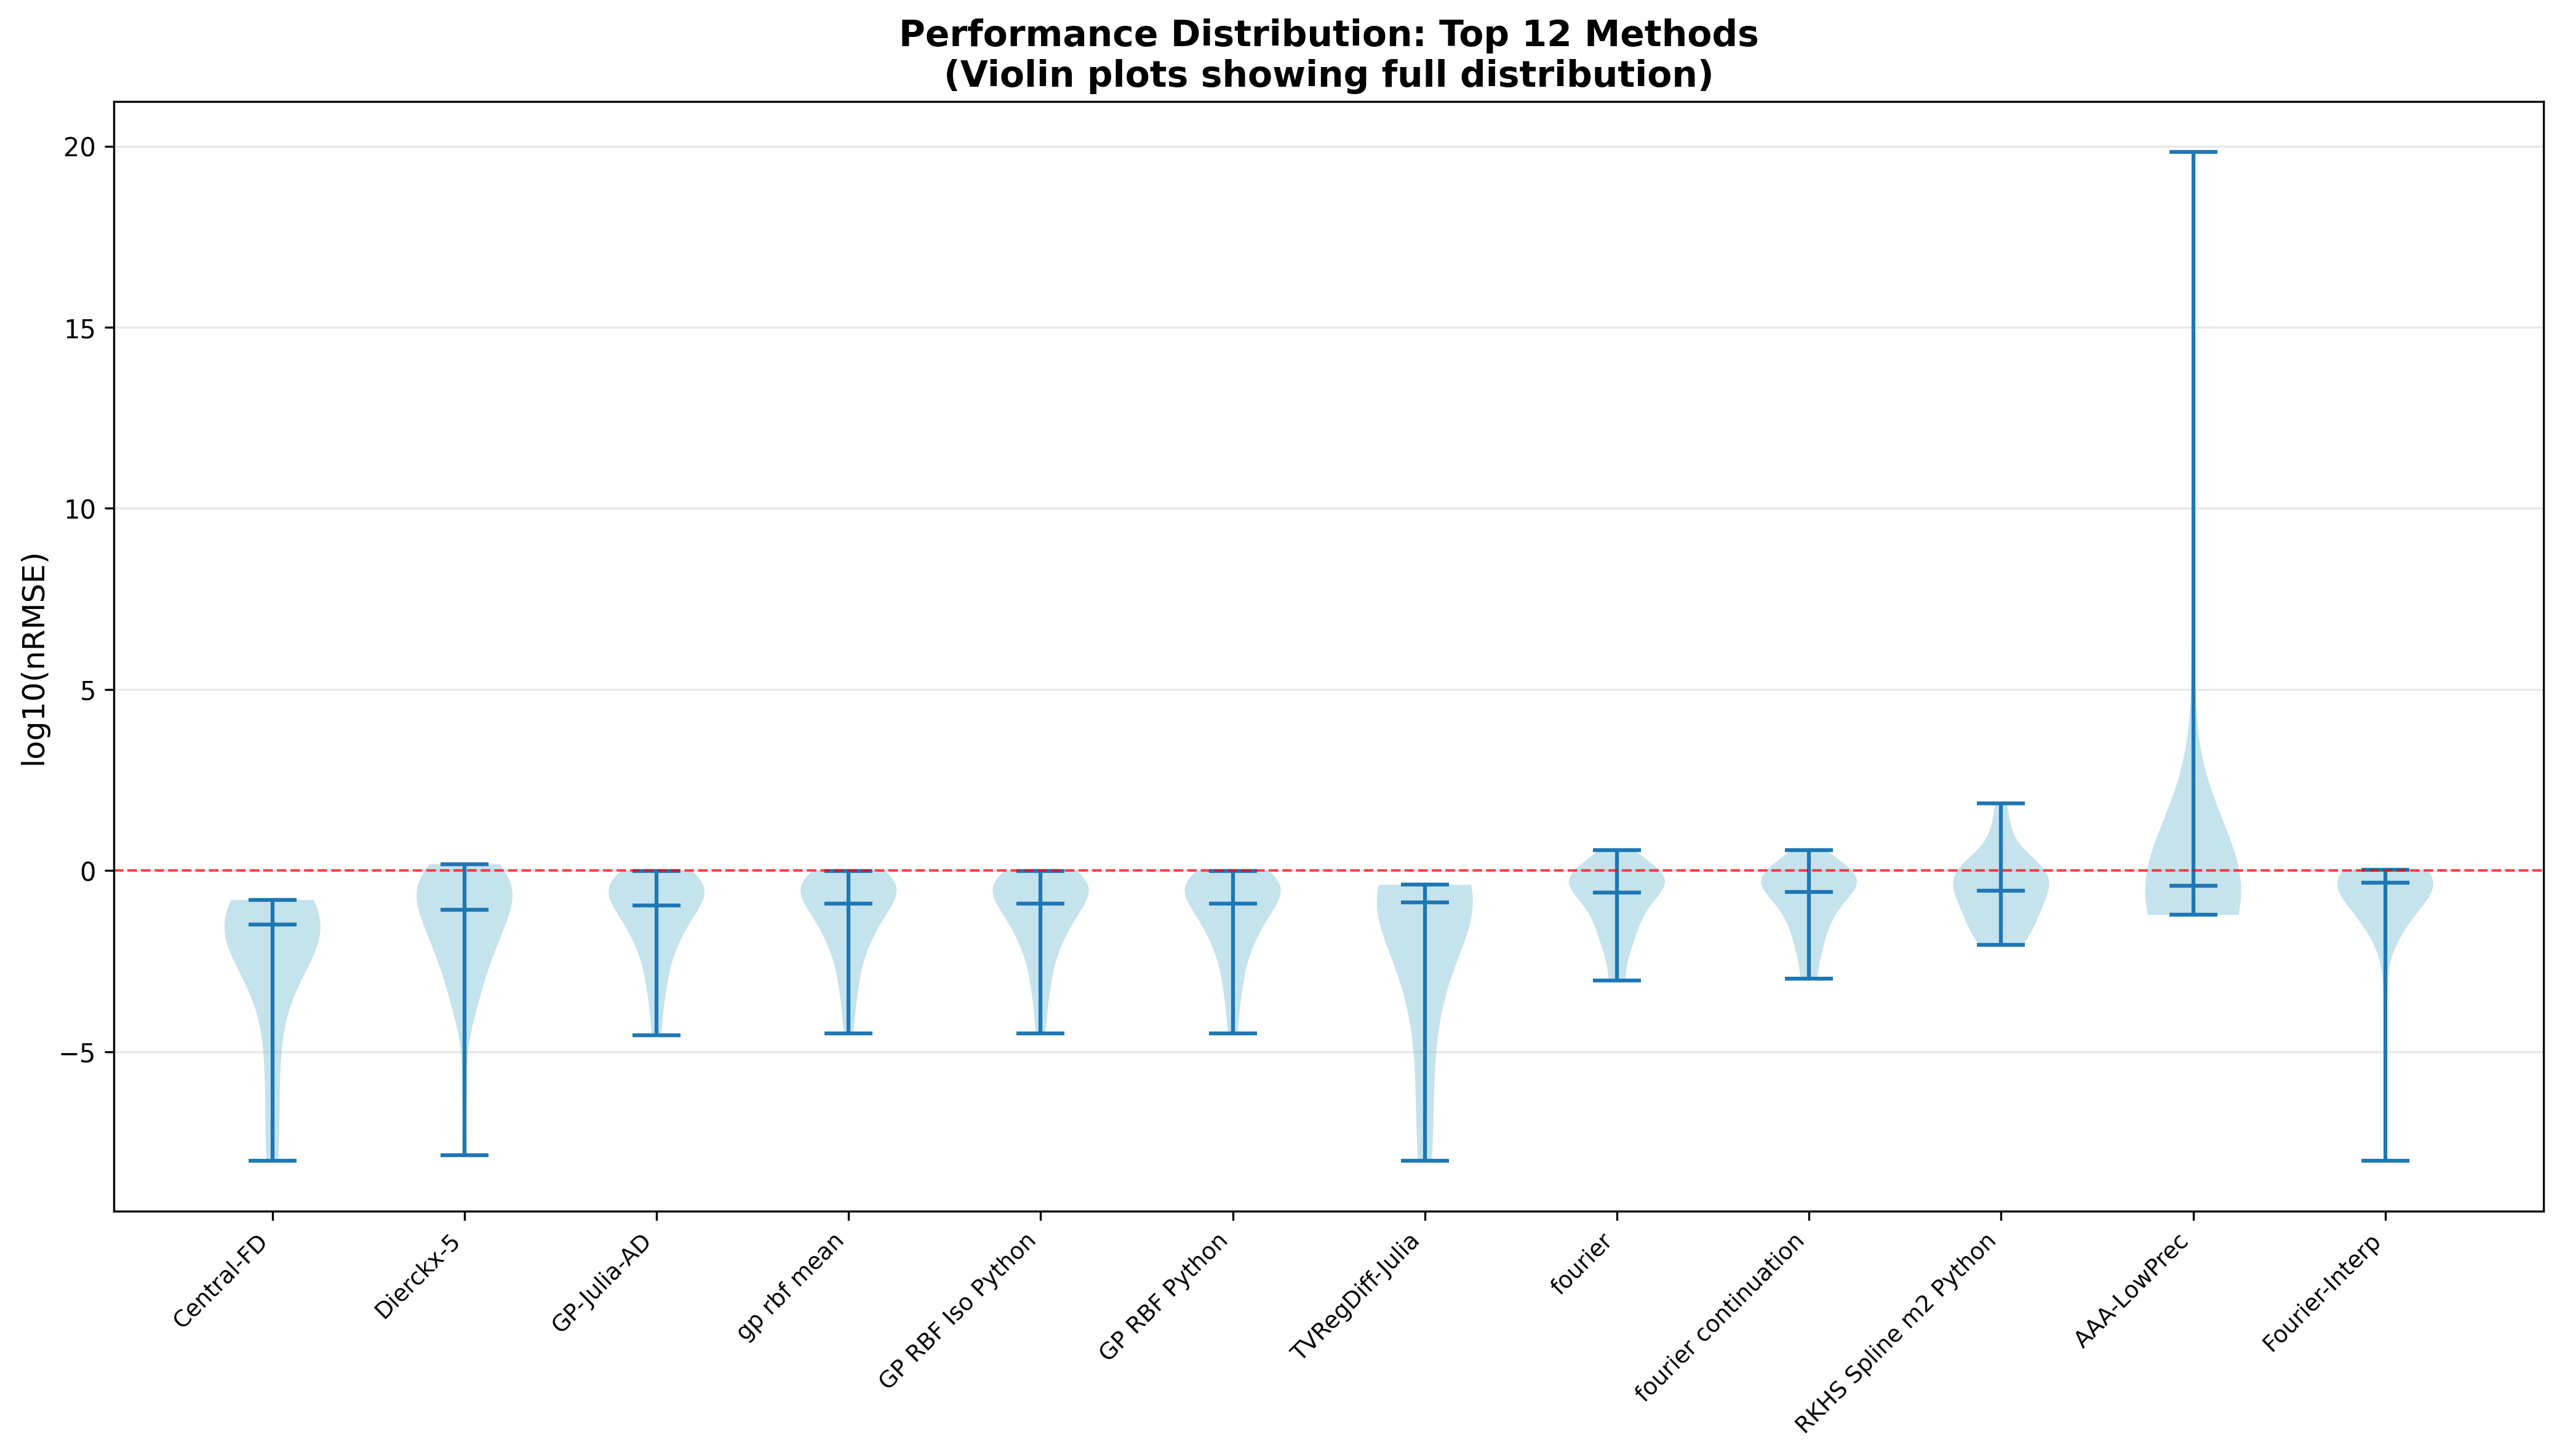
\includegraphics[width=\textwidth]{plot13_violin_top12.png}
\end{figure}

\clearpage

%==============================================================================
% PLOT 14
%==============================================================================

\section*{Plot 14: Heatmap Small Multiples (Method × Noise by Order)}

\textbf{What it shows:} One heatmap per derivative order showing method × noise performance

\textbf{Strengths:}
\begin{itemize}
    \item Complete view of method-noise interaction at each order
    \item 16 full-coverage methods shown
    \item Reveals noise sensitivity patterns
    \item Color scale consistent across panels
\end{itemize}

\textbf{Best for:} Comprehensive noise sensitivity analysis, identifying robust vs fragile methods

\begin{figure}[h]
\centering
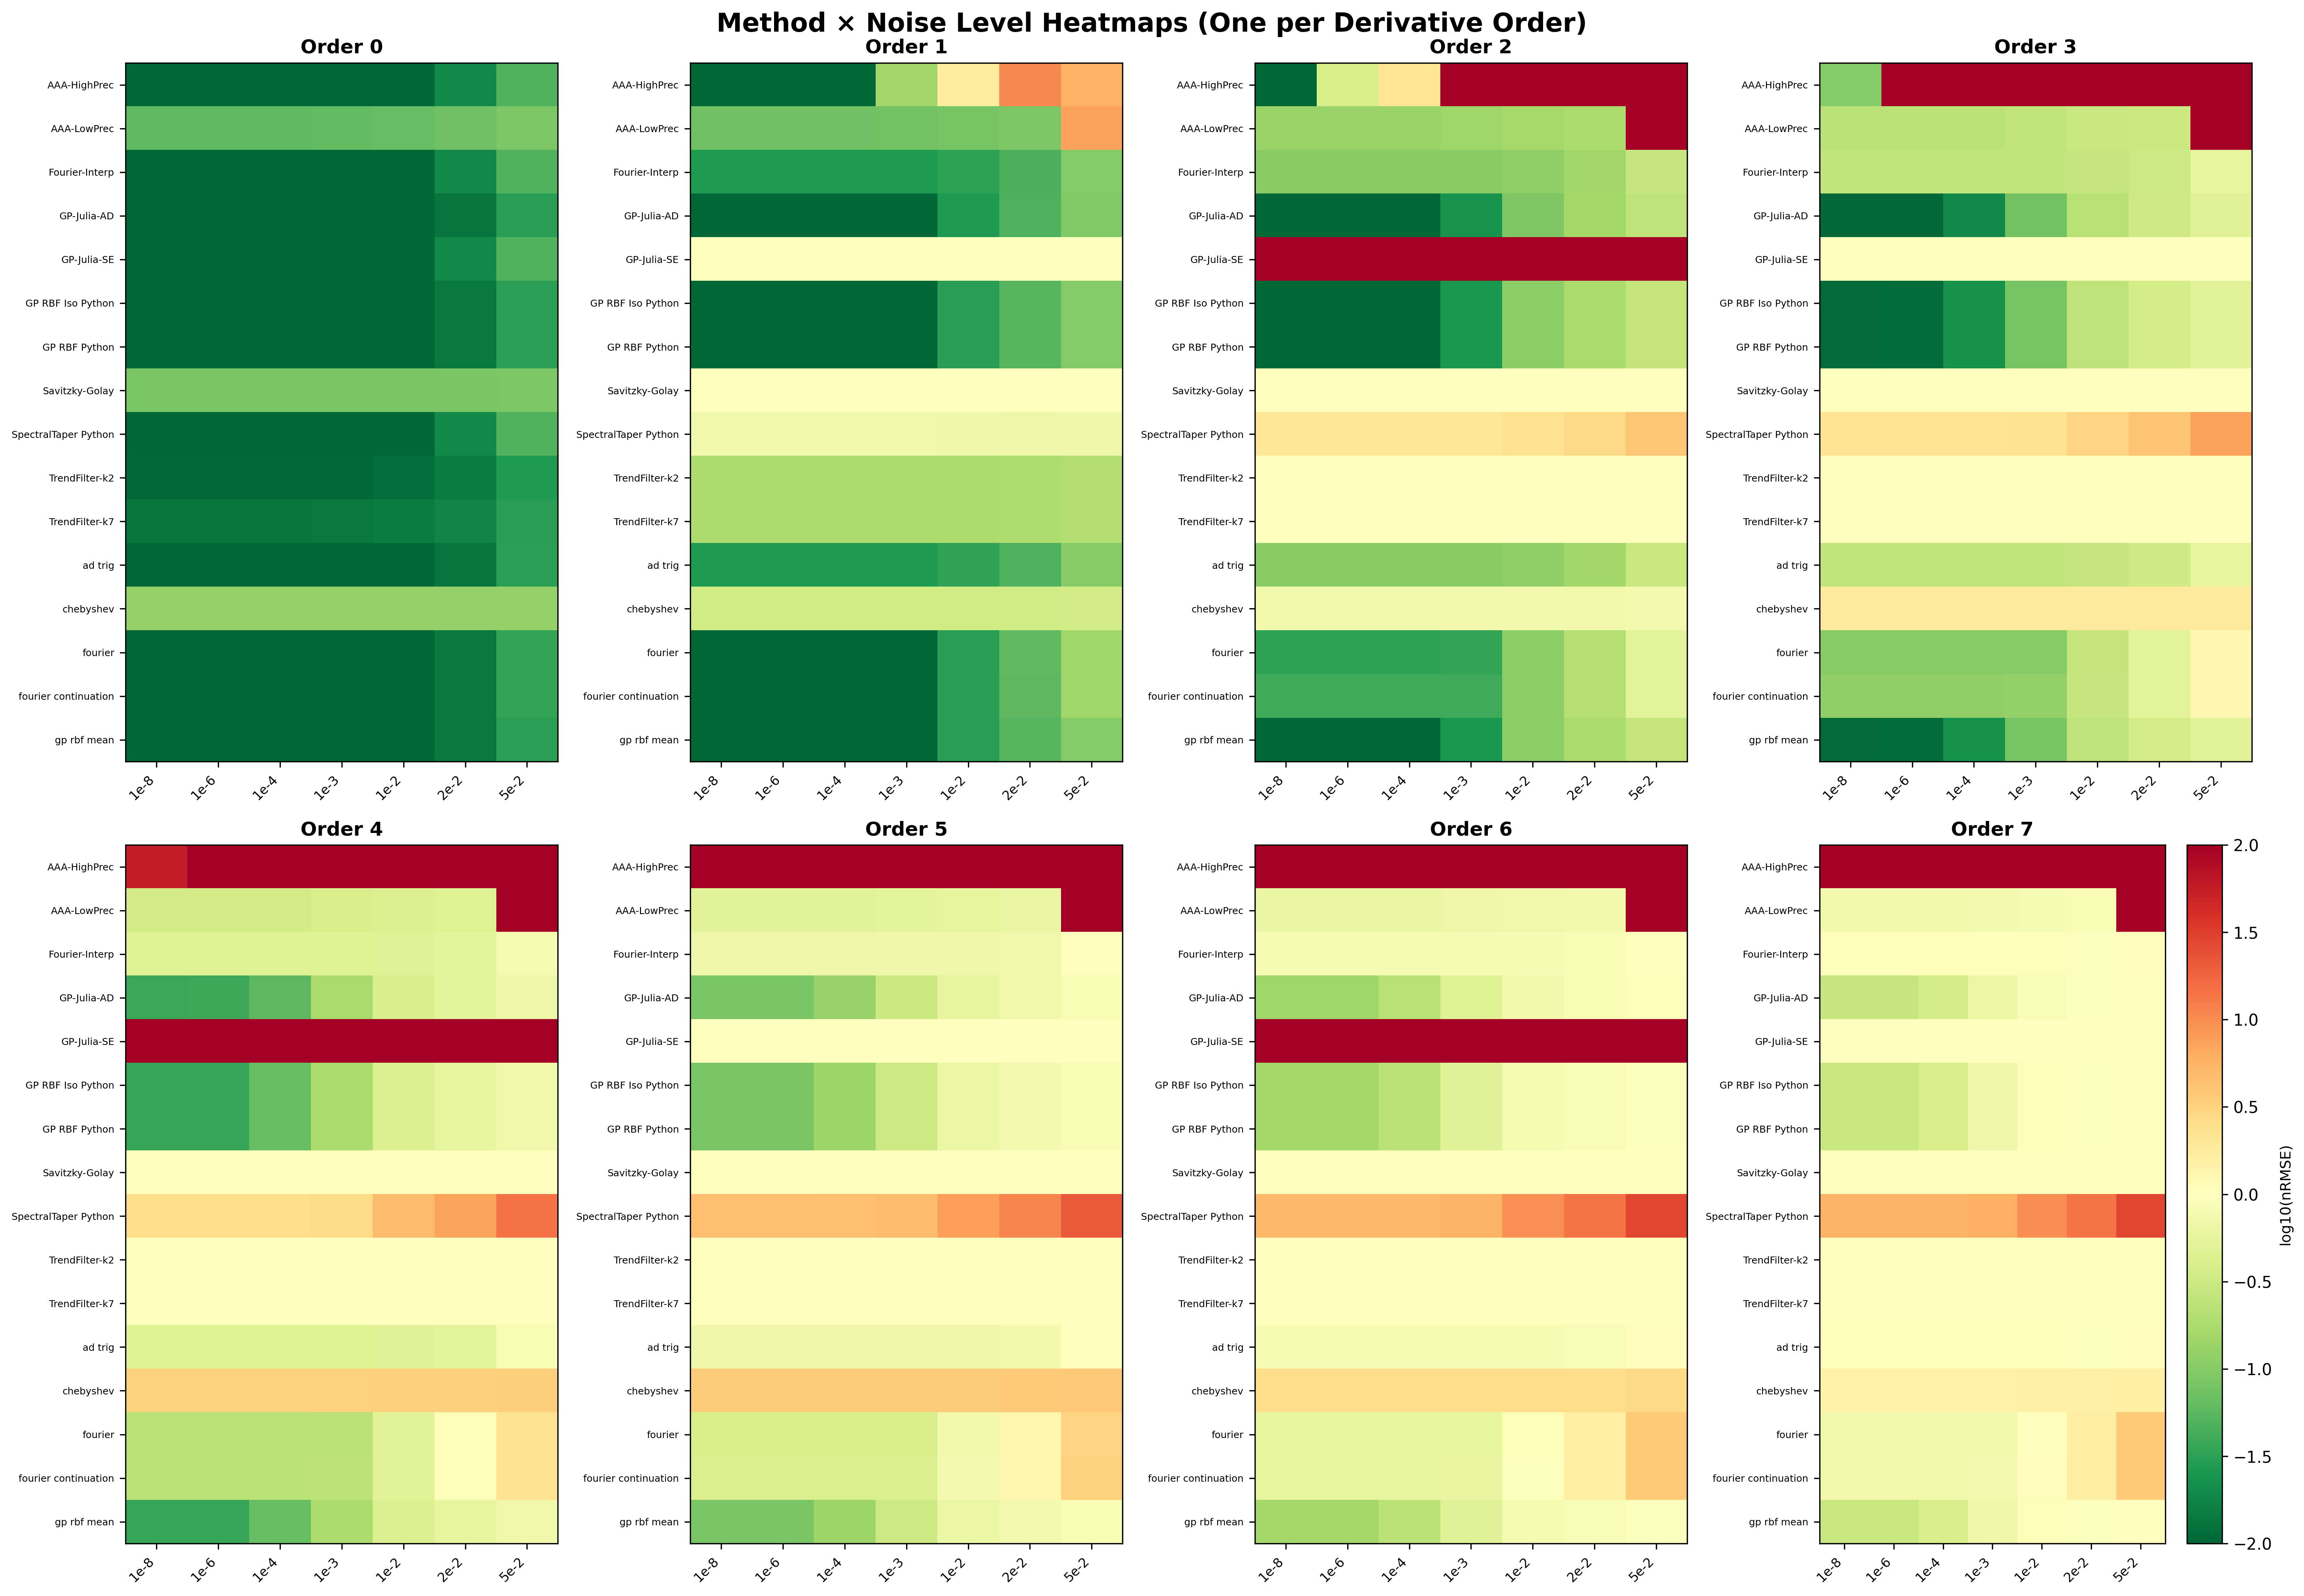
\includegraphics[width=\textwidth]{plot14_heatmap_multiples.png}
\end{figure}

\clearpage

%==============================================================================
% PLOT 15
%==============================================================================

\section*{Plot 15: Accuracy vs Robustness Scatter}

\textbf{What it shows:} Performance on easy conditions vs hard conditions

\textbf{Strengths:}
\begin{itemize}
    \item Identifies method archetypes (accurate, robust, both, neither)
    \item Lower-left quadrant = ideal (good at both)
    \item Category colors reveal algorithmic patterns
    \item Practical for method selection by priorities
\end{itemize}

\textbf{Best for:} Characterizing method strengths, supporting ``no universal best'' claim

\begin{figure}[h]
\centering
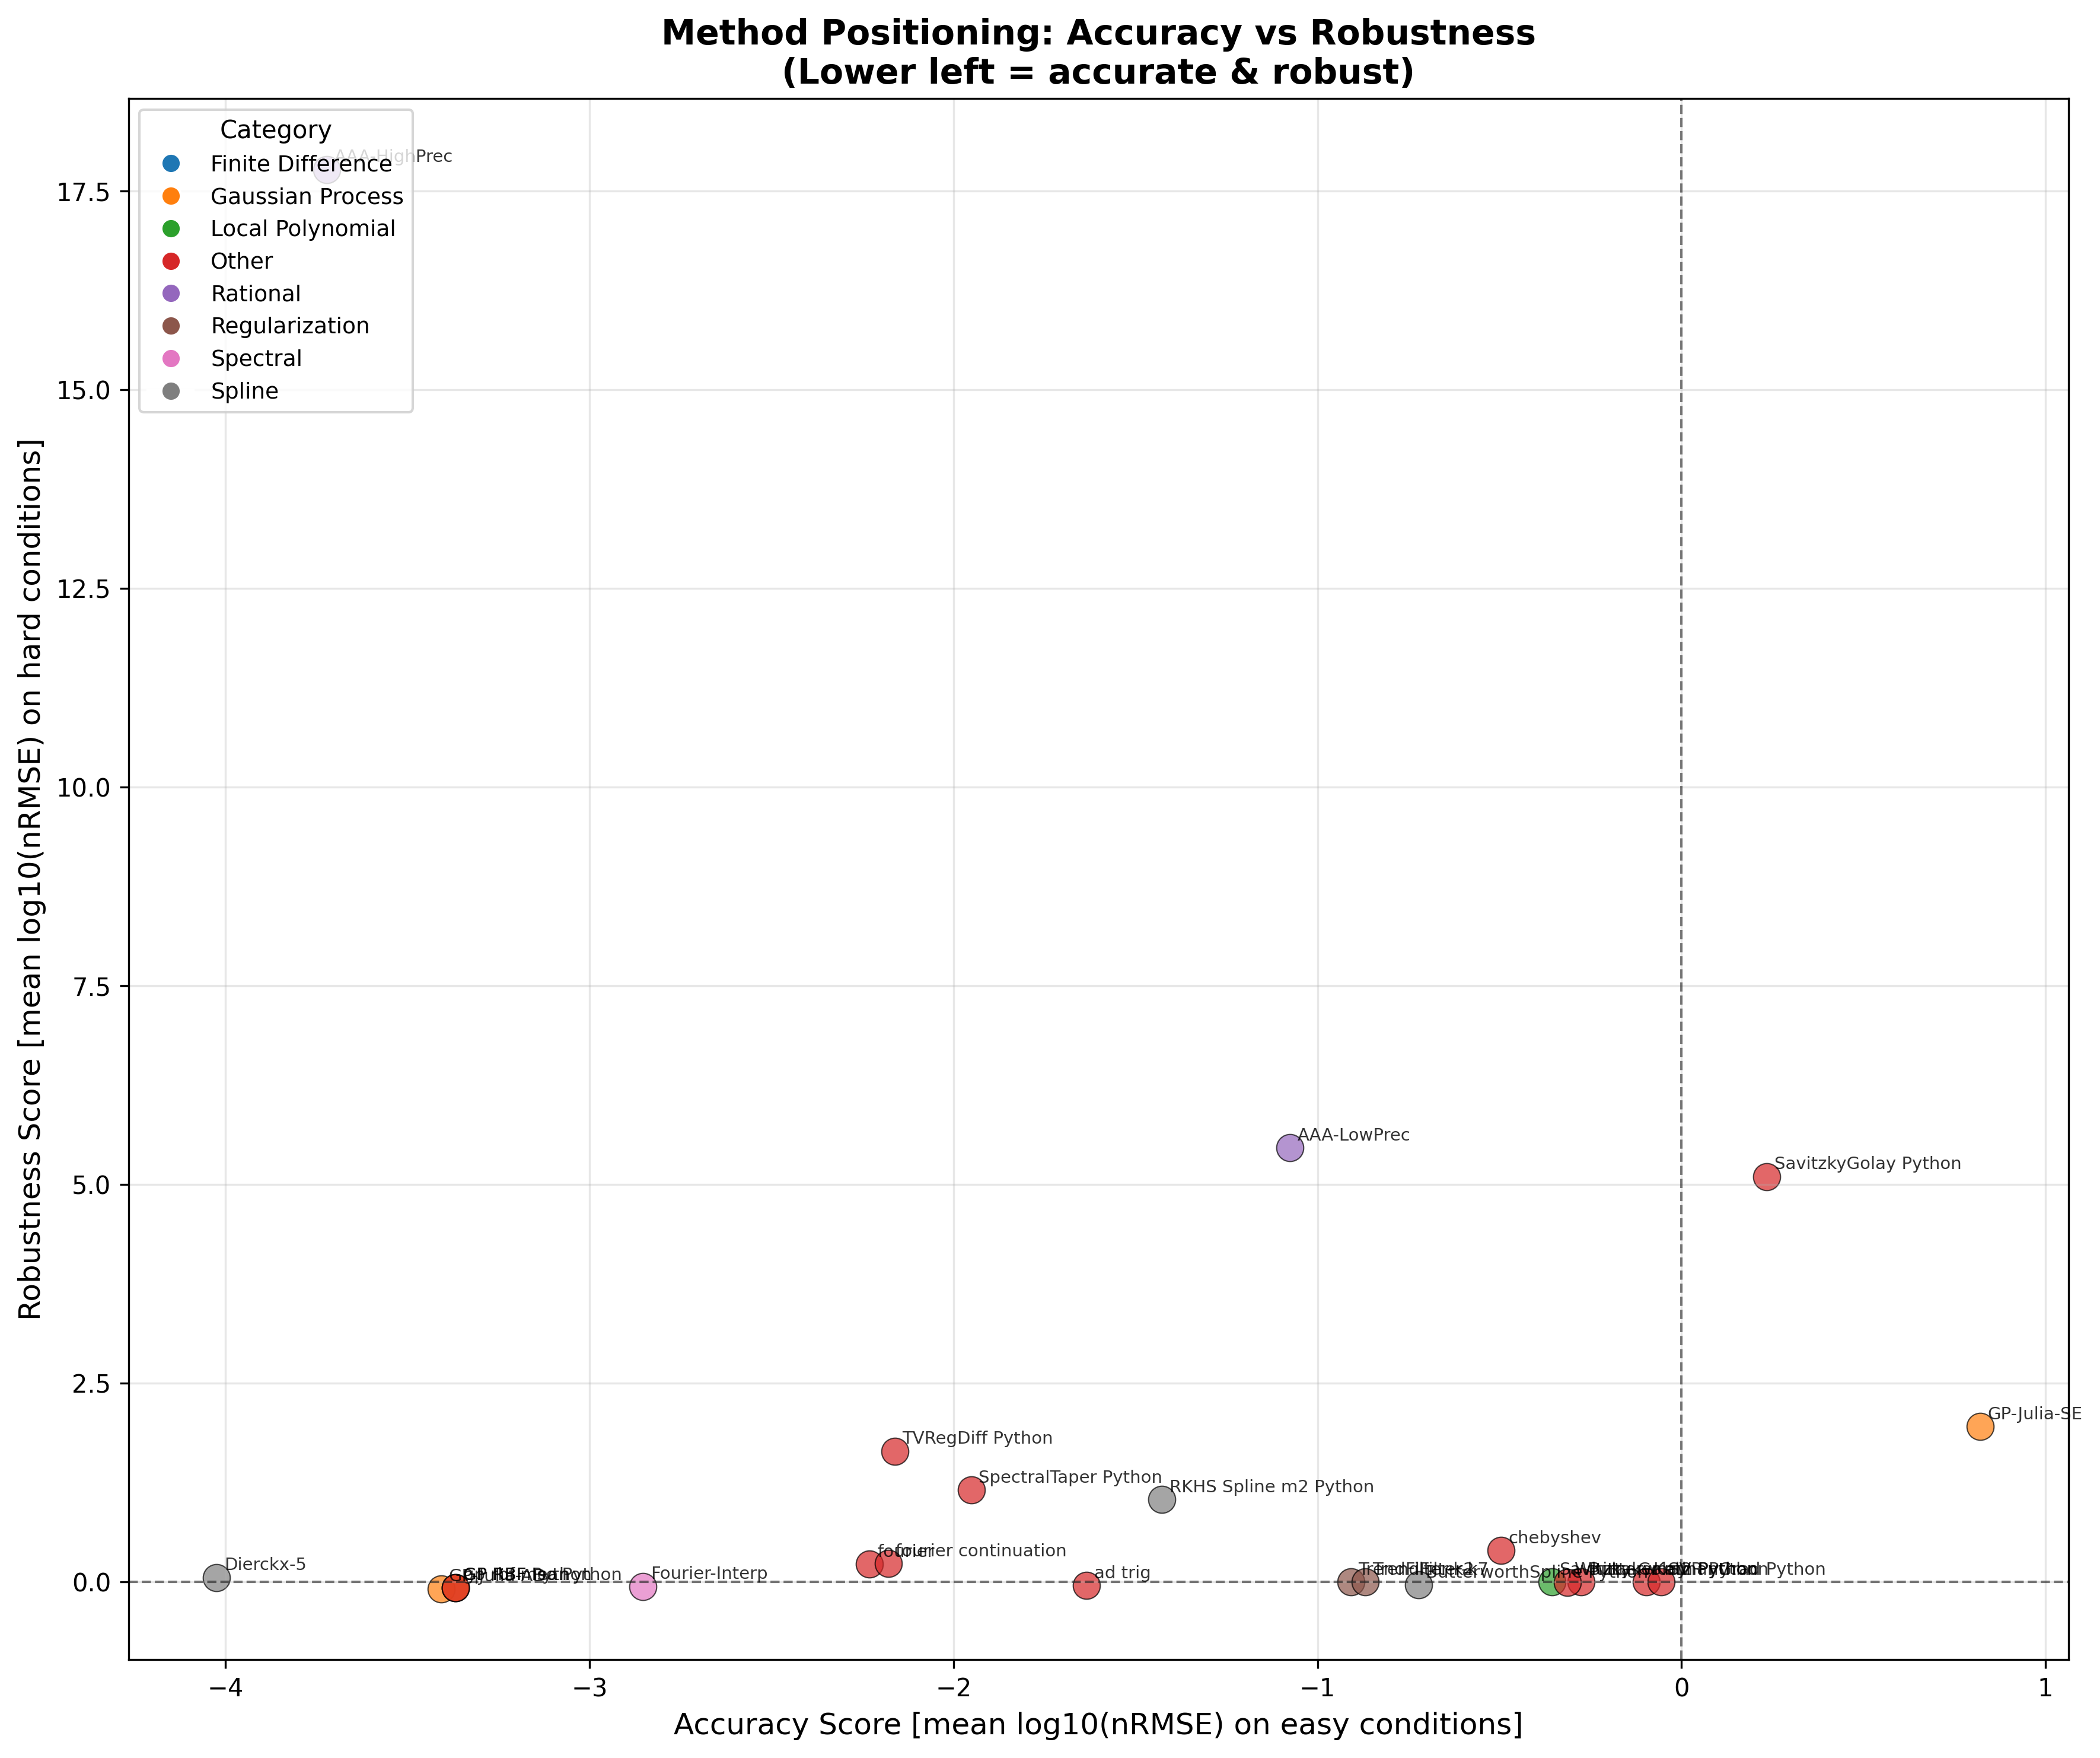
\includegraphics[width=\textwidth]{plot15_accuracy_robustness.png}
\end{figure}

\clearpage

%==============================================================================
% PLOT 16
%==============================================================================

\section*{Plot 16: High-Order Performance Only}

\textbf{What it shows:} Mean log10(nRMSE) at extreme challenge (orders 5-7 only)

\textbf{Strengths:}
\begin{itemize}
    \item Focuses on hardest test case
    \item Shows which methods remain viable at high orders
    \item Excludes ``easy'' conditions that inflate averages
    \item Clear ranking by robustness
\end{itemize}

\textbf{Best for:} High-order derivative applications, demonstrating GP superiority at extremes

\begin{figure}[h]
\centering
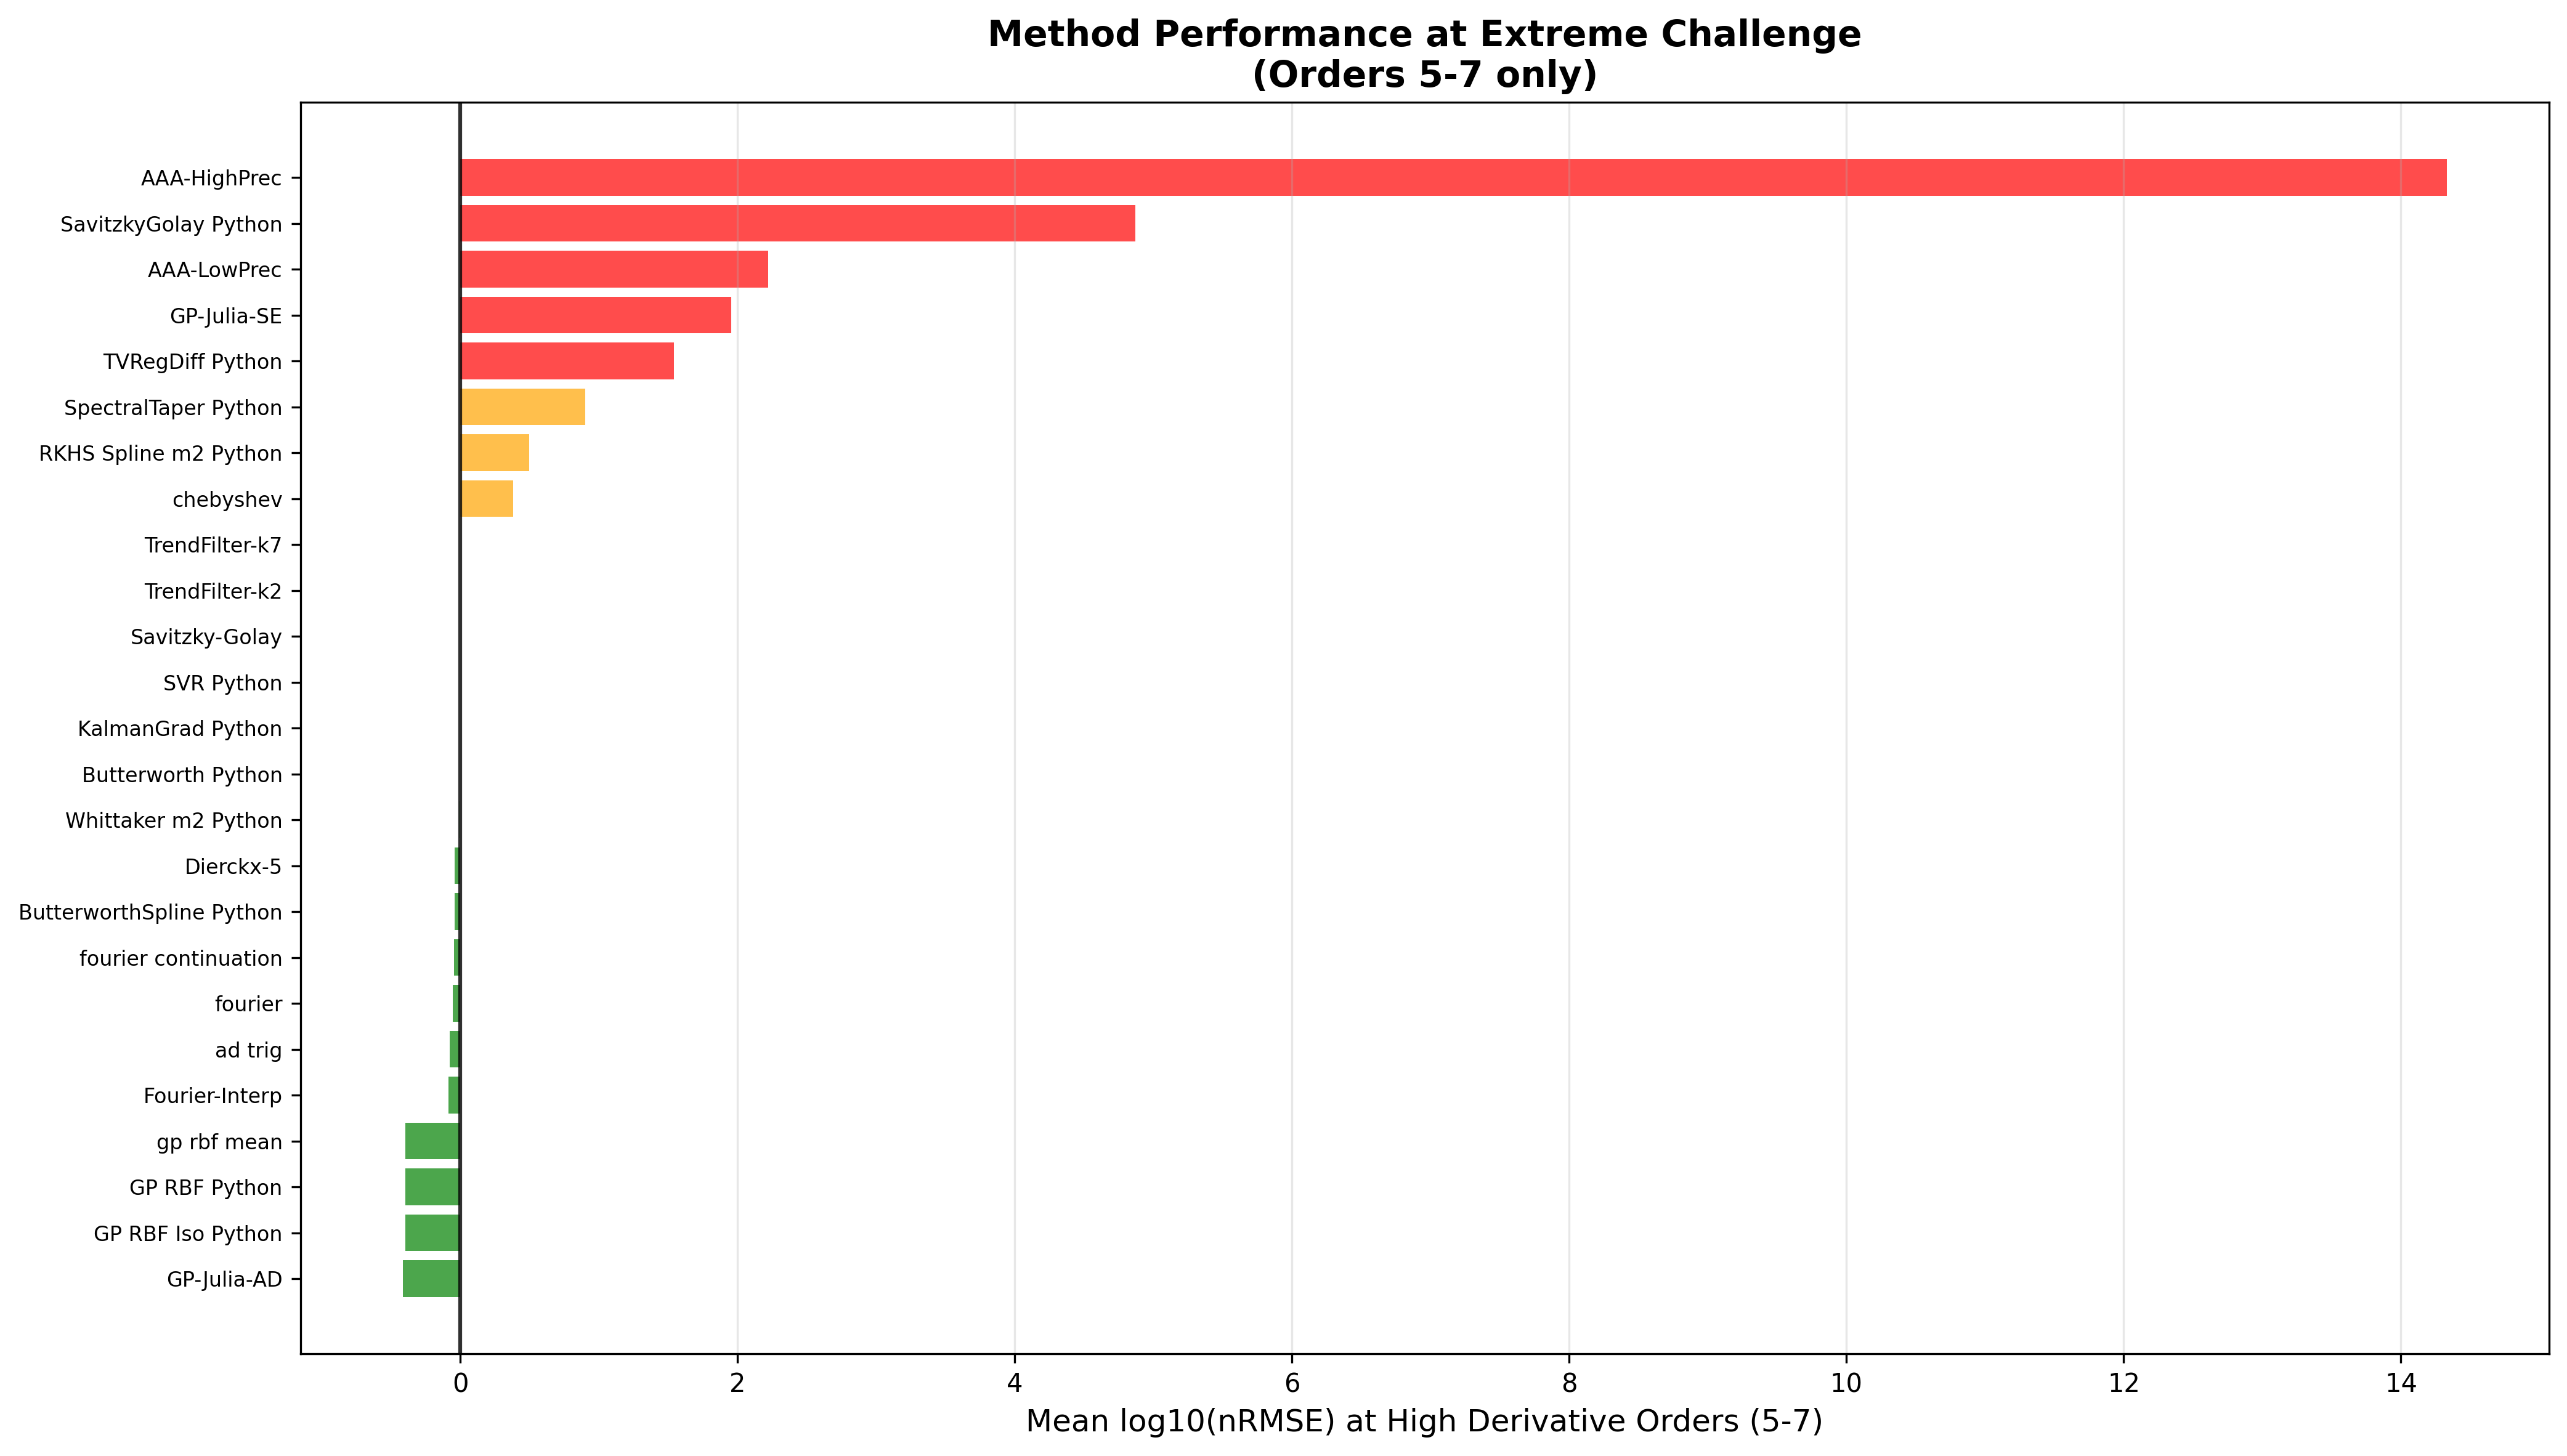
\includegraphics[width=0.85\textwidth]{plot16_high_order_only.png}
\end{figure}

\clearpage

%==============================================================================
% PLOT 17
%==============================================================================

\section*{Plot 17: Symlog Heatmap}

\textbf{What it shows:} nRMSE heatmap using symmetric log scale (handles extreme range better)

\textbf{Strengths:}
\begin{itemize}
    \item No capping/filtering - shows true values
    \item Symlog scale: linear near zero, log at extremes
    \item Preserves both small and large differences
    \item All 27 methods visible
\end{itemize}

\textbf{Best for:} When exact extreme values matter, unbiased visualization

\begin{figure}[h]
\centering
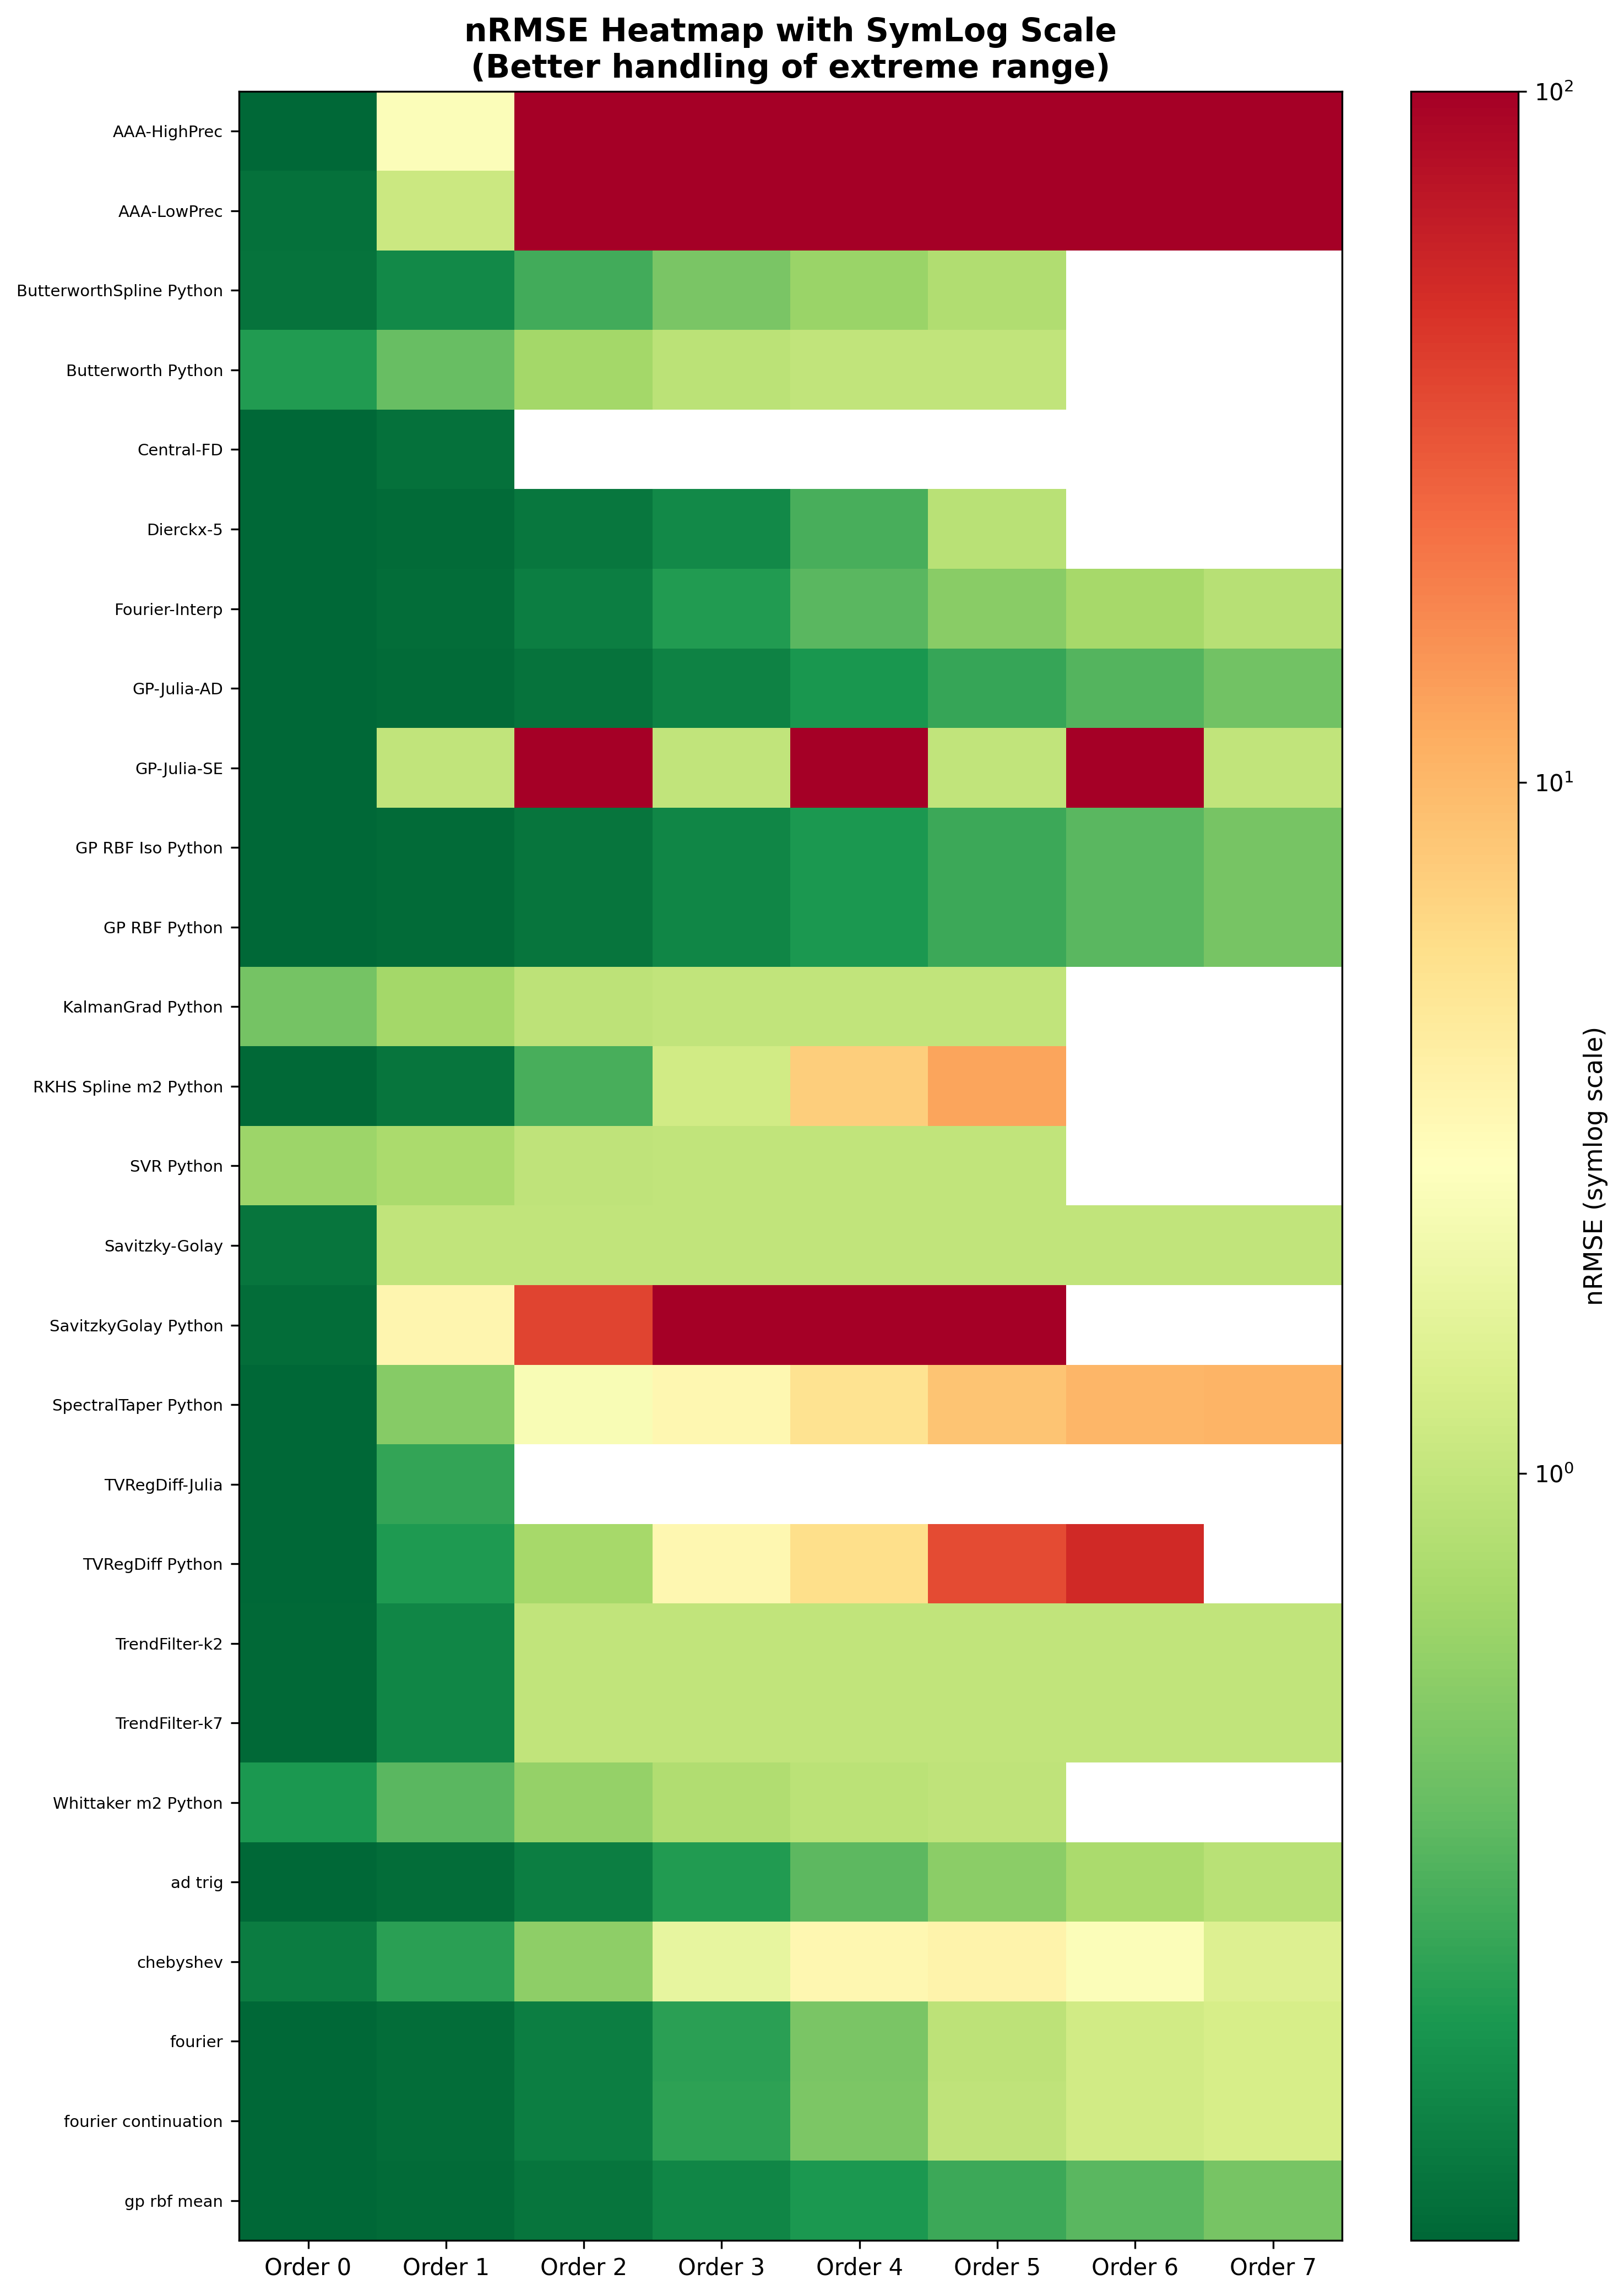
\includegraphics[width=0.85\textwidth]{plot17_symlog_heatmap.png}
\end{figure}

\clearpage

%==============================================================================
% PLOT 18
%==============================================================================

\section*{Plot 18: Viable Method Count Grid}

\textbf{What it shows:} Number of methods achieving nRMSE $<$ 1.0 for each (order, noise) condition

\textbf{Strengths:}
\begin{itemize}
    \item Shows problem difficulty from practitioner perspective
    \item Numbers in cells = method choices available
    \item Reveals ``easy'' vs ``hard'' regions
    \item Supports ``high order + high noise = few viable options''
\end{itemize}

\textbf{Best for:} Demonstrating problem difficulty gradient, method selection constraints

\begin{figure}[h]
\centering
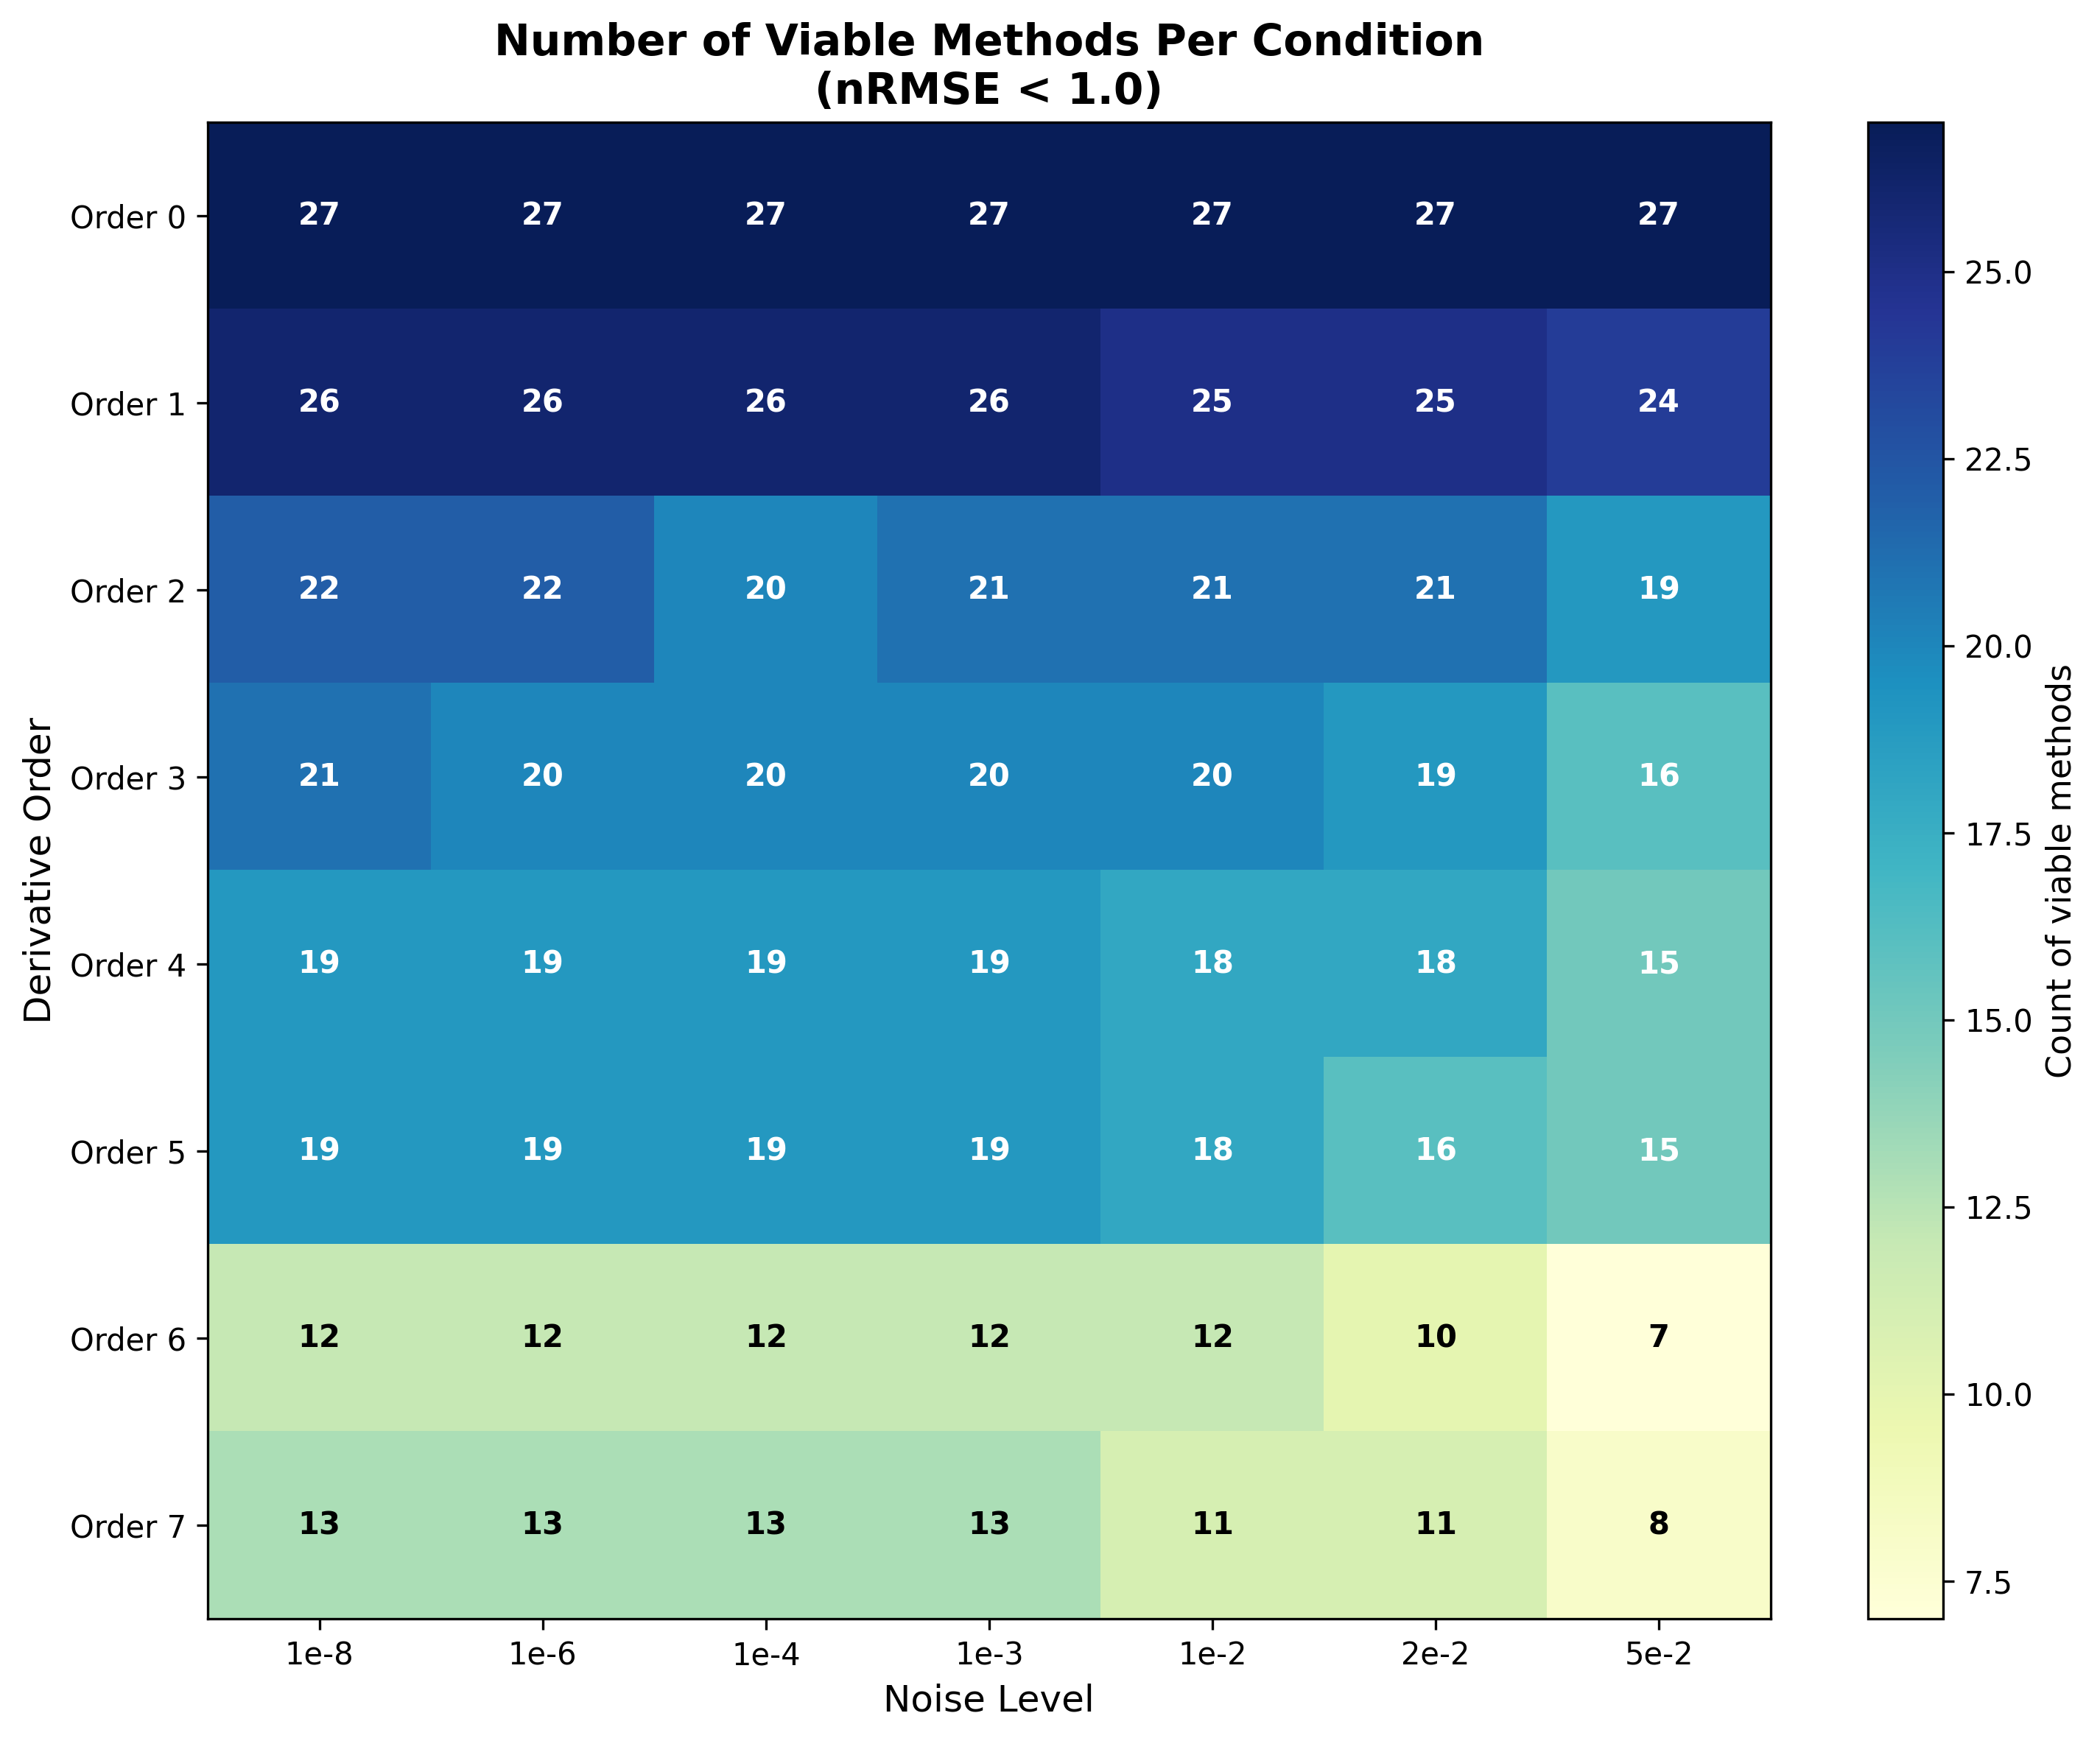
\includegraphics[width=0.85\textwidth]{plot18_viable_count_grid.png}
\end{figure}

\clearpage

%==============================================================================
% PLOT 19
%==============================================================================

\section*{Plot 19: Ridge Plot}

\textbf{What it shows:} Stacked density plots showing performance distribution evolution across orders

\textbf{Strengths:}
\begin{itemize}
    \item Beautiful, intuitive visualization
    \item Shows distribution shift (not just mean shift) with order
    \item Reveals bimodality, skew changes
    \item Visually striking for presentations
\end{itemize}

\textbf{Best for:} High-impact visualizations, showing difficulty progression intuitively

\begin{figure}[h]
\centering
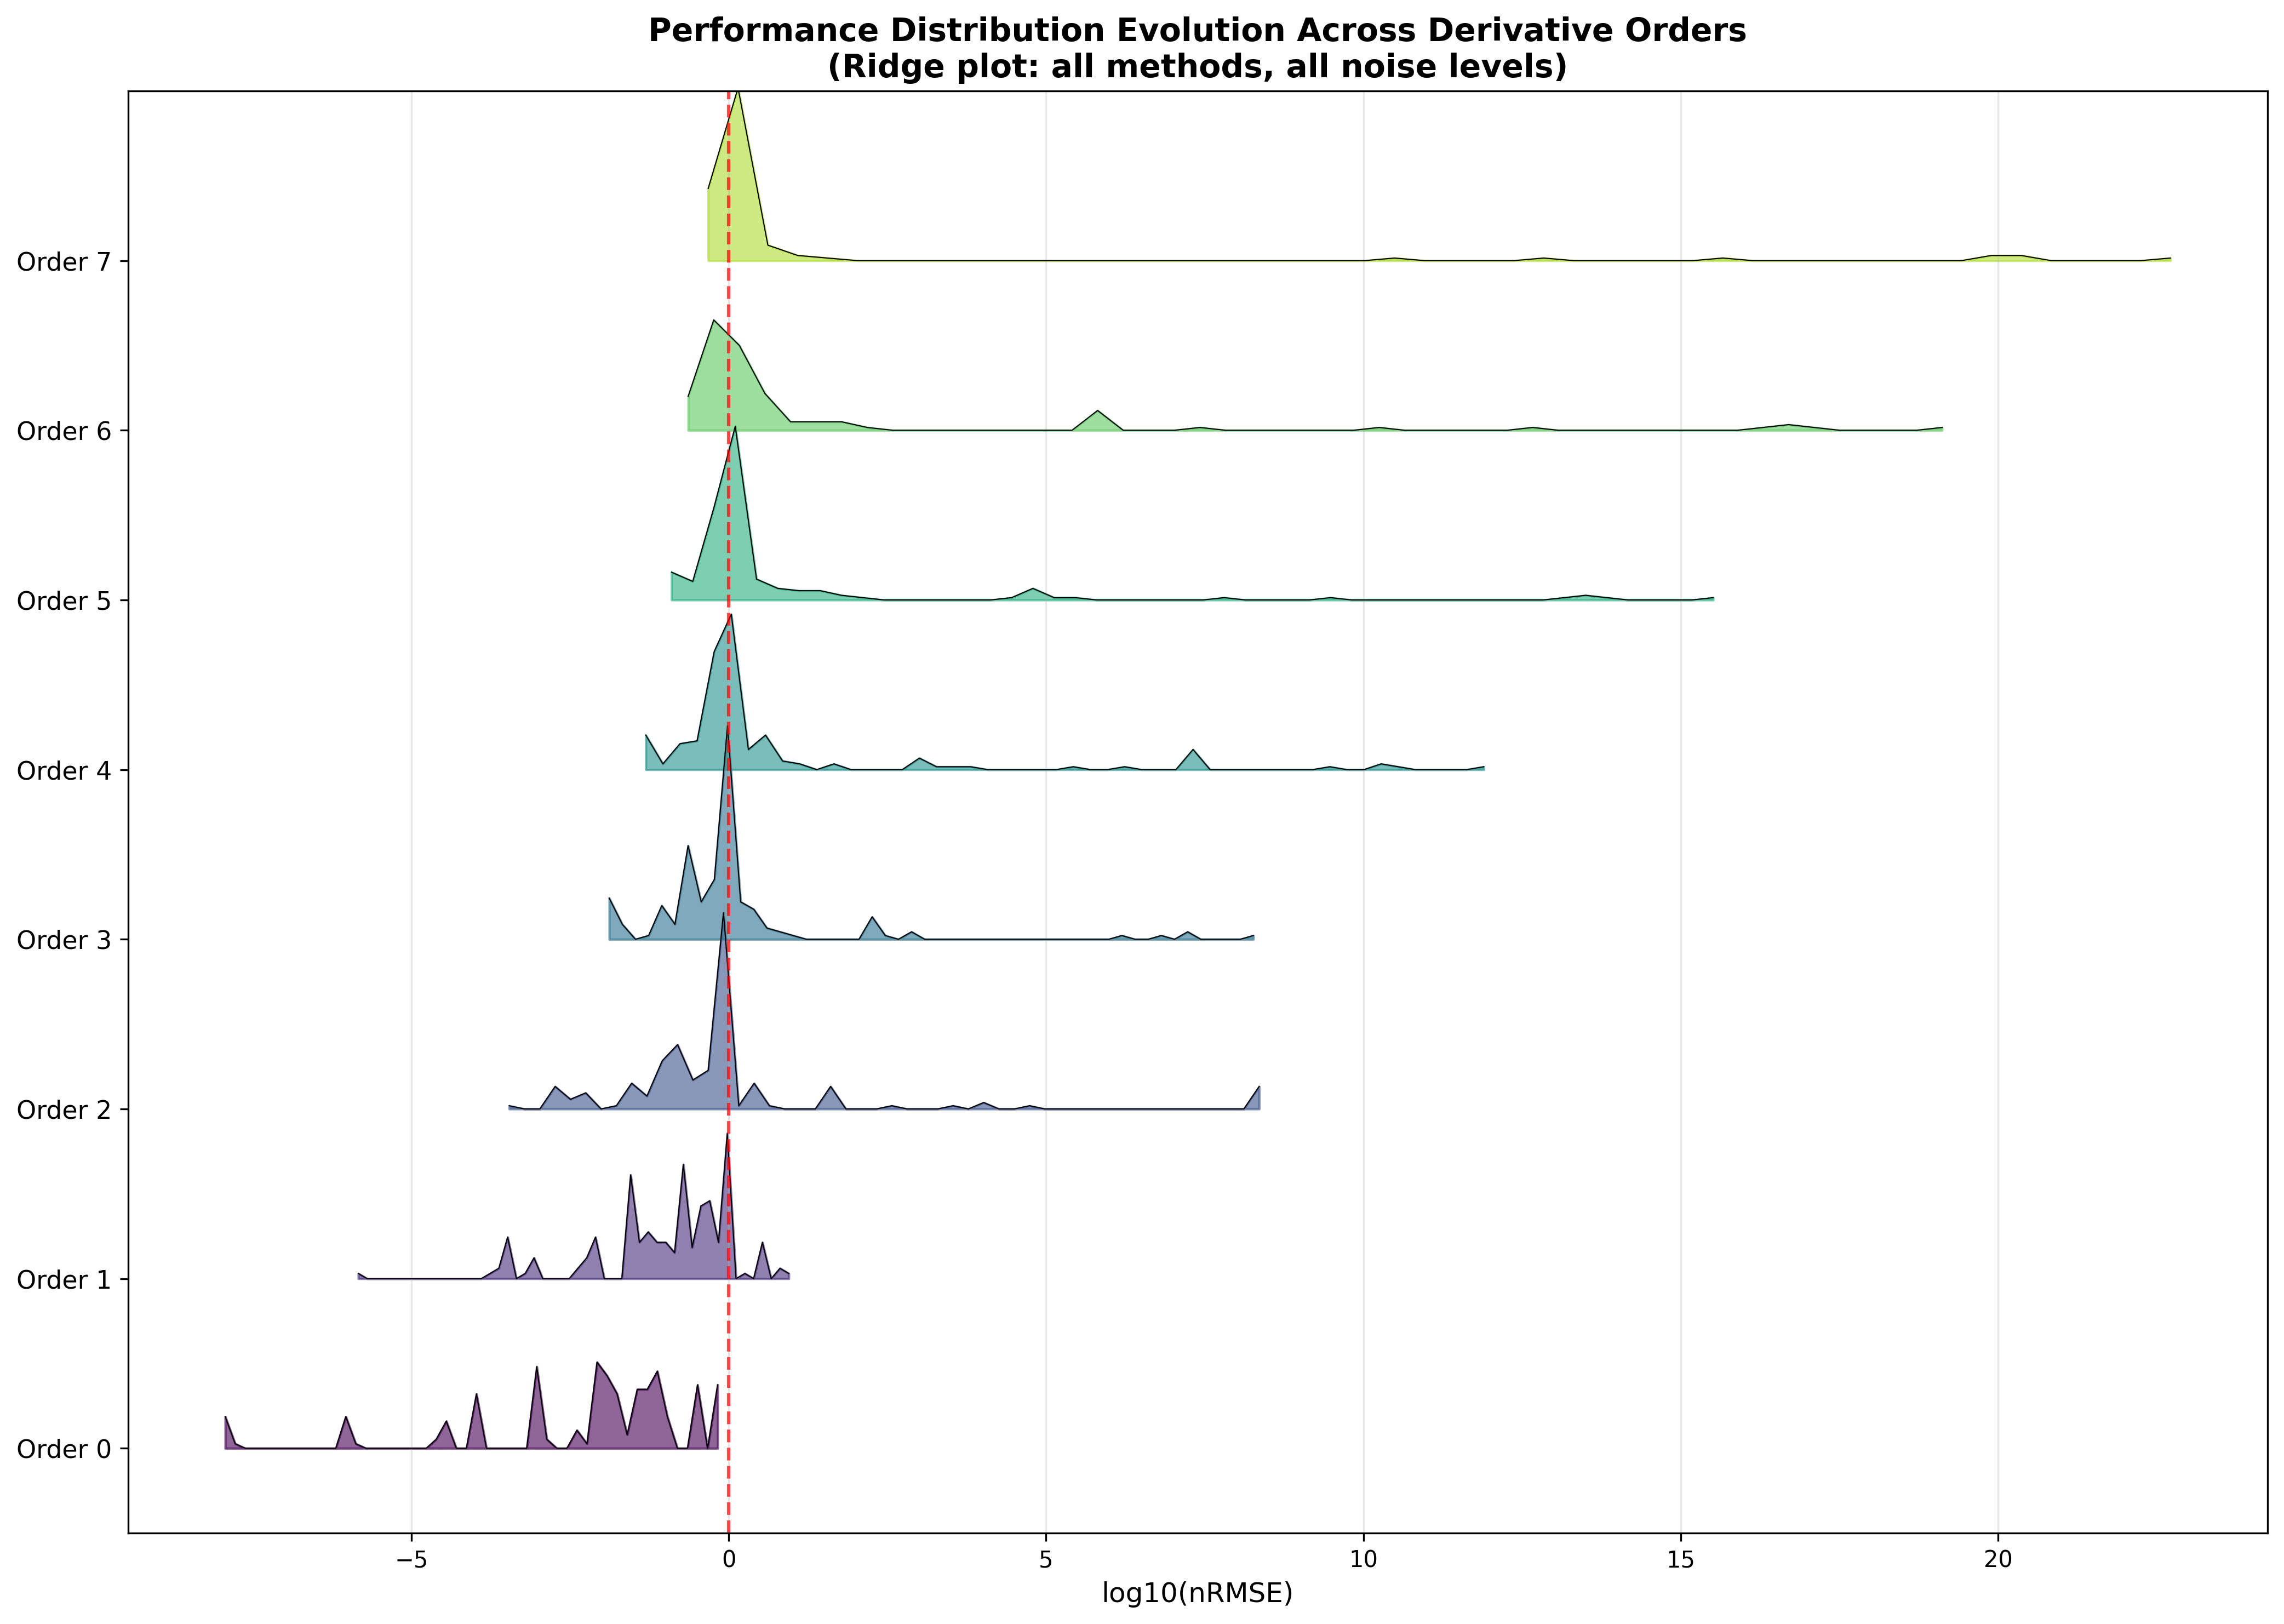
\includegraphics[width=\textwidth]{plot19_ridge_plot.png}
\end{figure}

\clearpage

%==============================================================================
% PLOT 20
%==============================================================================

\section*{Plot 20: Coverage Map}

\textbf{What it shows:} Which methods were tested at which (order, noise) combinations

\textbf{Strengths:}
\begin{itemize}
    \item Documents coverage bias issue
    \item Green = tested, Gray = not tested, Red = catastrophic failure
    \item Shows method scope limitations
    \item Supports ``only 16/27 have full coverage'' claim
\end{itemize}

\textbf{Best for:} Transparency about test coverage, explaining partial-coverage exclusions

\begin{figure}[h]
\centering
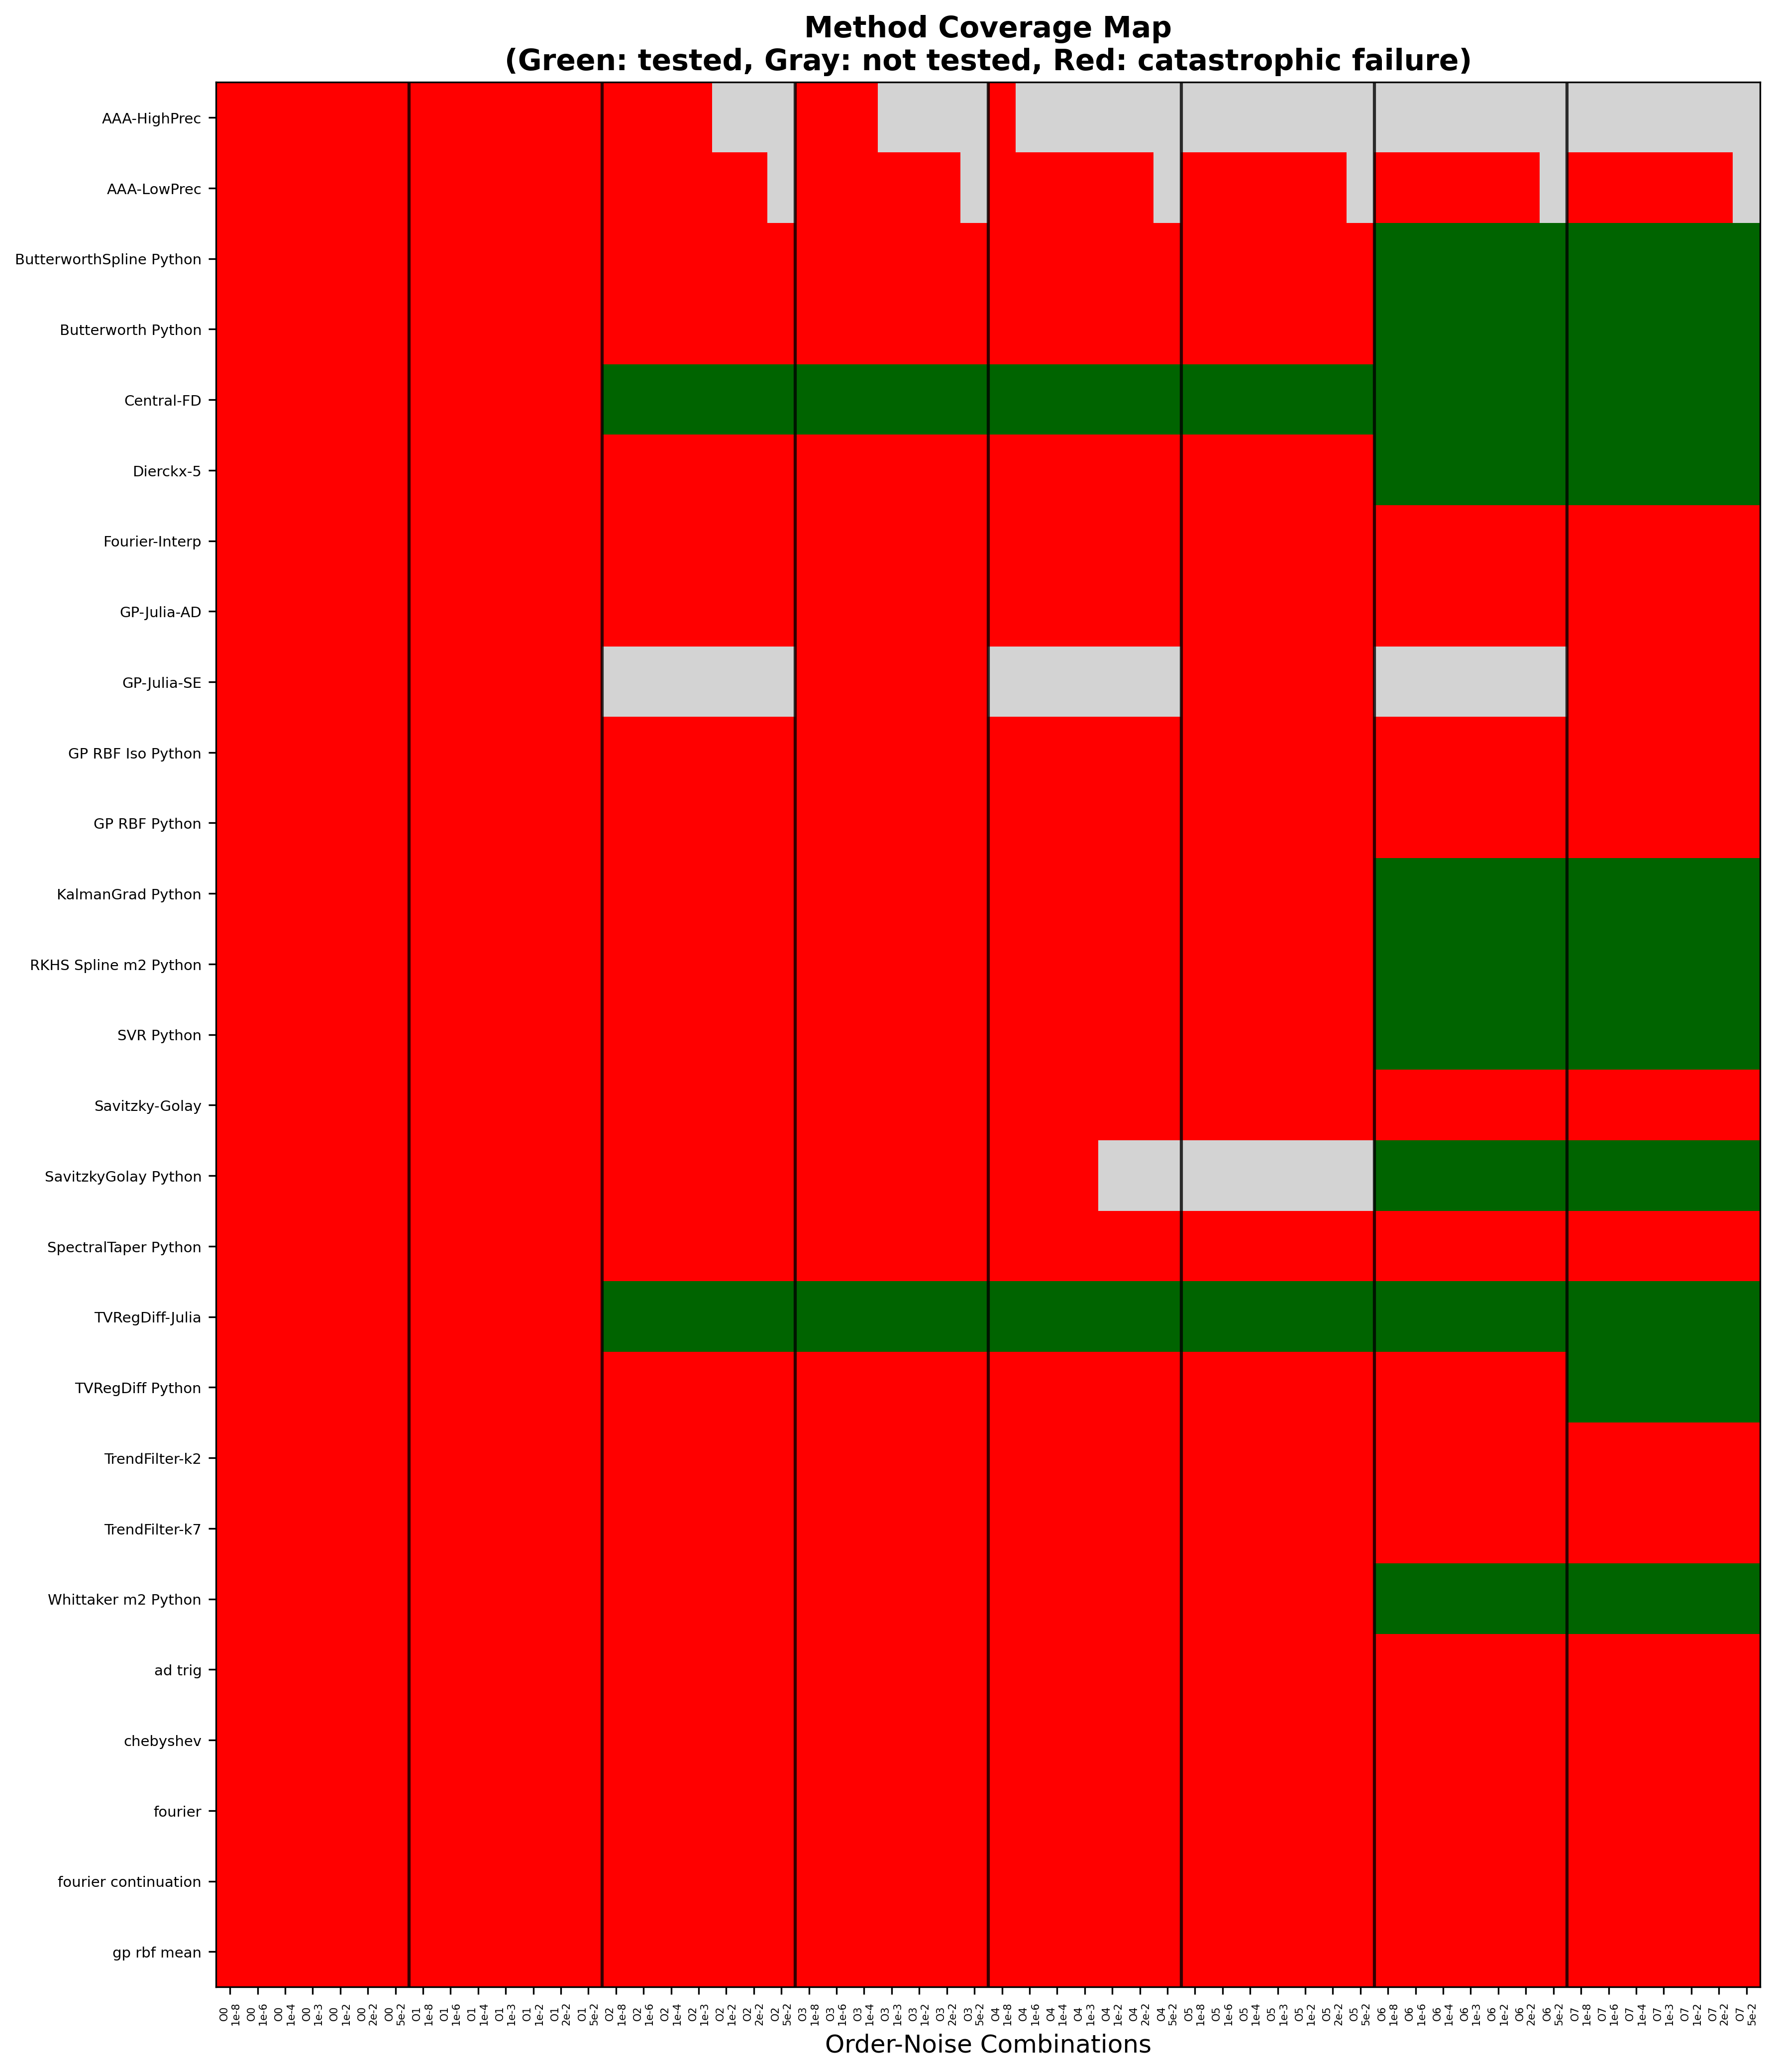
\includegraphics[width=0.9\textwidth]{plot20_coverage_map.png}
\end{figure}

\clearpage

%==============================================================================
% RECOMMENDATIONS
%==============================================================================

\section*{Recommendations by Use Case}

\subsection*{For Main Paper (pick 3-5):}
\begin{itemize}
    \item \textbf{Plot 2} (order degradation) - supports ``order is primary driver''
    \item \textbf{Plot 5} (ranking) - supports ``GP-Julia-AD best overall''
    \item \textbf{Plot 7} (failure rate) - supports ``AAA catastrophic failure''
    \item \textbf{Plot 10} (best method grid) - practical method selection
    \item \textbf{Plot 15} (accuracy vs robustness) - supports ``no universal best''
\end{itemize}

\subsection*{For Supplementary Material (pick 8-12):}
\begin{itemize}
    \item All of the above, plus:
    \item \textbf{Plot 1} (box plots all methods) - complete overview
    \item \textbf{Plot 4} (small multiples) - detailed noise analysis
    \item \textbf{Plot 8 or 9} (category comparison) - algorithmic insights
    \item \textbf{Plot 11} (stacked bars) - balanced success/failure view
    \item \textbf{Plot 14} (heatmap multiples) - comprehensive interaction effects
    \item \textbf{Plot 18} (viable count) - difficulty visualization
    \item \textbf{Plot 20} (coverage map) - methodological transparency
\end{itemize}

\subsection*{For Presentations (visually striking):}
\begin{itemize}
    \item \textbf{Plot 3} (heatmap) - color gradient pattern
    \item \textbf{Plot 10} (best method grid) - practical lookup table
    \item \textbf{Plot 15} (scatter) - method archetypes
    \item \textbf{Plot 19} (ridge plot) - beautiful distribution evolution
\end{itemize}

\subsection*{For Reviewers (addresses specific concerns):}
\begin{itemize}
    \item \textbf{Plot 6} (mean vs std) - consistency claim
    \item \textbf{Plot 12} (vs baseline) - relative performance
    \item \textbf{Plot 16} (high-order only) - extreme challenge
    \item \textbf{Plot 20} (coverage) - methodological rigor
\end{itemize}

\end{document}
